\documentclass[11pt,dvipsnames]{memoir}
\usepackage[dvipsnames,table]{xcolor}
\usepackage[utf8]{inputenc}
\usepackage[T1]{fontenc}
\usepackage[american]{babel}
\usepackage{amsmath, amssymb, amsthm}
\usepackage{todonotes}
\usepackage{graphicx}
\usepackage{tikz}
\usepackage{hhline}
\usepackage{physics}
\usepackage{mathtools}
\usepackage{tikz}
\usepackage{bm}
\usepackage[linesnumbered,ruled]{algorithm2e}
\usepackage{listings}
\usepackage{float}
\usepackage[url=false,style=phys,biblabel=brackets,maxbibnames=10,backend=bibtex,sorting=none]{biblatex}
\usepackage{subcaption}
\usepackage[font={small}]{caption}
\usepackage{xfrac}
\usepackage{multirow}
\usepackage{makecell}
\usepackage[chapter]{minted}
\usepackage[colorlinks=true, linkcolor=blue]{hyperref}

% ================================================================================
% Configuration of subfigures
% ================================================================================
\DeclareCaptionLabelFormat{subfigure}{\textbf{#2.}}
\captionsetup[subfigure]{
  font={bf}, skip=1pt, singlelinecheck=false, labelformat=subfigure, subrefformat=parens
}
\captionsetup{subrefformat=subfigure}

% ================================================================================
% Colors for table headers
% ================================================================================
\colorlet{theader}{ProcessBlue!30}
\colorlet{tsubheader}{ProcessBlue!20}

\addbibresource{my_papers_phd.bib}
\addbibresource{ref.bib}


% ================================================================================
% Theorem environments
% ================================================================================
\theoremstyle{definition}
\newtheorem{example}{Example}[chapter]
\newtheorem{lemma}{Lemma}
\newtheorem{theorem}{Theorem}


% ================================================================================
% Symbols to be used in figures' captions, they correspond to the markers
% ================================================================================
\DeclareRobustCommand\tikzdot{\tikz[overlay,yshift=0.5ex] \fill[blue!90] (0.ex,0.ex) circle (0.3ex);}
\DeclareRobustCommand\tikzcircle{\tikz[overlay,yshift=0.5ex] \draw[red,thick] (0.ex,0.ex) circle (0.4ex);}
\DeclareRobustCommand\tikzquad{\tikz[overlay,yshift=0.ex,xshift=0.1ex] \draw[green,thick] (0.ex,0.ex) rectangle (1ex,1ex);}

% ================================================================================
% Title page info
% ================================================================================
\title{Validation and benchmarking of quantum annealing technology}
\author{Konrad Jałowiecki}
\date{January 2022}


% ================================================================================
% Styles and definitions
% ================================================================================
\def\clockop{\altmathcal{C}}
\def\coefmatrix{\altmathcal{A}}

\linespread{1.15}
% minted style
\usemintedstyle{default}
\colorlet{lstbg}{black!80}

\AtBeginBibliography{\small}

\ExecuteBibliographyOptions{doi=false}

\DeclareFieldFormat{title}{#1}
\DeclareFieldFormat[article]{title}{{\itshape #1}}

\allowdisplaybreaks[4]

\begin{document}

\begin{titlingpage}
  \begin{center}
    
\includegraphics[width=0.4\textwidth]{figures/iitis_logo}\\
    \vspace{0.5em}
    \textsc{\large Institute of Theoretical and Applied Informatics, Polish Academy of Sciences}
    \vspace*{1in}
    \hrule
    \vspace*{0.5em}
    \textsc{\huge Validation and benchmarking of quantum annealing technology}
    \vspace*{0.5em}
    \hrule
    \vspace*{1em}
    \textsc{\large Doctoral dissertation}
    \par
    \vspace{1.5in}
    {\large mgr Konrad \textsc{Jałowiecki}}\\
    \vspace{0.25in}
    Supervisor:\\ dr hab. Bartłomiej Gardas\\
    \vspace{0.25in}
    Co-supervisor:\\ dr hab. inż. Łukasz Pawela\\
    \vfill
    {Gliwice, \today}
  \end{center}
\end{titlingpage}

\frontmatter

\tableofcontents*
\newpage
\chapter{Acknowledgements}

I am deeply grateful to my supervisor, dr hab. Bartłomiej Gardas, whose unwavering support and insightful guidance have been instrumental in shaping this doctoral thesis. His expertise, encouragement, and mentorship have been invaluable, and I am truly fortunate to have had the opportunity to work under his supervision.

I would also like to express my sincere appreciation to my co-supervisor, dr hab. inż. Łukasz Pawela, for his constructive feedback, especially in the field of software engineering. His expertise and willingness to share knowledge have significantly enriched the quality of this thesis.

I would also like to express my gratitude to all my colleagues from the Institute who contributed to this thesis via many fruitful conversations I had with them. In particular, I would like to thank Krzysztof Domino for sharing his knowledge and expertise in the railway dispatching field.

Additionally, I extend my deepest gratitude to my friends, Alexander Juda and Michał Stęchły, for taking the time to read parts of this thesis. Their valuable feedback contributed greatly to improving the readability and overall quality of this work.

This project was partially supported by the National Science Center (NCN), Poland, under Projects: Sonata Bis 10, No. 2020/38/E/ST3/00269
and The National Centre for Research and Development (NCBR), Poland, under Project No. POIR.01.01.01-00-0061/2. I would also like to thank The Quantum Data Center Corporation for providing me with access to several GPUs used for benchmarks presented in this thesis.

%%% Local Variables:
%%% mode: latex
%%% TeX-master: "main"
%%% End:

%\addtocontents{toc}{\setlength{\cftchapterindent}{\cftchapternumwidth}}
\chapter{Published work}

\begin{refsection}
\nocite{Jaowiecki2020,Rams2021,JALOWIECKI2021107728,e25020191}
\printbibliography[heading=none]
\end{refsection}

%%% Local Variables:
%%% mode: latex
%%% TeX-master: "main"
%%% End:

%\addtocontents{toc}{\setlength{\cftchapterindent}{\cftchapternumwidth}}
\chapter{Abstract}

In this thesis, we focus on the problem of validating and benchmarking quantum annealers in a
practical context. To this end, we propose two algorithms for solving real-world problems and test how
well they perform on the current generation of quantum annealers. The first algorithm allows for
solving the dynamics of quantum systems (or, in fact, any dynamical systems). The second of the proposed
algorithms is suitable for solving a particular family of railway dispatching problems: the delay
and conflict management on single-track railway lines. We assess the performance of those
algorithms on the current generation of D-Wave quantum annealers with the assistance of two novel,
classical strategies for solving an Ising model also presented in the thesis. The first, tensor
network-based approach is a heuristic algorithm specifically tailored for solving instances defined
on Chimera-like graphs, thus making it ideal for providing a baseline with which the results from
physical annealers can be compared. The other presented approach is a massively parallel
implementation of the exhaustive search through the whole solution space, also known as the
brute-force approach. Although the brute-force approach is limited to moderate instance sizes, it
has the advantage of being able to compute the low energy spectrum and certify the solutions. Thus,
it can be used to obtain additional insight into the solution space structure. The results obtained
in our experiments suggest that already present-day quantum annealers are capable of solving a
subset of the aforementioned optimization problems. In particular, we show that the D-Wave annealers
are capable of capturing the dynamics of a simple two-level quantum system in a specific regime of
parameters, and can be used to obtain good-quality solutions for instances of railway conflict
management problems. Finally, our findings make it clear that the current generation of the D-Wave
annealers is far from perfect. We discuss problem instances for which the annealers failed to find
a good or even feasible solution. We also provide, where possible, a plausible explanation of why
some of the presented problems might be hard for the annealers.
%%% Local Variables:
%%% mode: latex
%%% TeX-master: "../main"
%%% End:

\chapter{Streszczenie}

\begin{otherlanguage}{polish}
  W niniejszej pracy skupiamy się na problemie walidowania i benchmarkowania
  wyżaraczy kwantowych w praktycznym kontekście. W tym celu, przedstawiamy dwa
  algorytmy służące do rozwiązywania rzeczywistych problemów, oraz sprawdzamy,
  jak dobrze sprawdzają się na obecnej generacji wyżaraczy kwantowych. Pierwszy z
  algorytmów pozwala na rozwiązywanie dynamiki kwantowych układów (lub, w gruncie
  rzeczy, dowolnych układów dynamicznych). Drugi z przedstawianych algorytmów
  może skolei zostać użyty do rozwiązywania pewnego podzbioru kolejowych
  problemów dyspozytorski: zarządania opóźnieniami i konfliktami w sieciach
  kolejowych o jednej linii. Oceny działania obu w.w. algorytmów na bieżącej
  generacji wyżaraczy D-Wave dokonujemy z pomocą dwóch, nowatorskich, klasycznych
  strategii rozwiązywania szkieł spinowych Isinga, które również prezentujemy w
  niniejszej rozprawie. Pierwszym z nich jest opierający się na sieciach tensorowych
  heurystyczny algorytm stworzony specjalnie do rozwiązywania szkieł spinowych
  zdefiniowanych na grafach przypominających topologię Chimera, co sprawia, że
  idealnie nadaje się do wyznaczania referencyjnych rozwiązań, do których można
  porównać wyniki z fizycznych wyżarzaczy. Drugim z prezentowanych podejść jest
  masywnie równoległa implementacja wyczerpującego przeszukiwania całej
  przestrzeni rozwiązań, tzw. brute-force. Mimo, że użycie algorytmu brute-force
  jest ograniczone do instancji o niewielkich rozmiarach, posiada on tę zaletę,
  że może wyznaczać niskoenergetyczne spektrum, oraz certyfikować rozwiązania. W
  związku z~tym, algorytm przeszukiwania wyczerpującego może slużyć do uzyskania
  dodatkowego wglądu w strukturę przestrzeni rozwiązań. Wyniki otrzymane w
  naszych eksperymentach sugerują, że już współczesne wyżarzacze są w stanie
  uchwycić dynamikę prostych, dwupoziomowych układów kwantowych w specyficznym
  reżimie parametrów, oraz mogą znaleźć dobrej jakości rozwiązania instancji
  kolejowych problemów. Wreszcie, nasze eksperymenty pokazują jasno, że obecna
  generacja wyżaraczy D-Wave nie jest idealna. Wymieniamy instancje problemów,
  dla których wyżarzanie nie potrafily znaleźść wysokojakościowych, lub nawet
  dopuszczalnych rozwiązań. Tam gdzie to możliwe, omawiamy również możliwe
  wyjaśnienie dlaczego niektóre z prezentowanych instancji mogą być dla wyżaraczy
  wymagające.
\end{otherlanguage}

%%% Local Variables:
%%% mode: latex
%%% TeX-master: "../main"
%%% End:


\mainmatter

\chapter{Introduction}
The previous century has witnessed what is now called the digital revolution.
The introduction of digital computers dramatically altered multiple aspects of
our lives. In particular, almost every area of science benefitted hugely from
the increasingly available computational power \cite{winsberg}. Physics was no
exception, and numerical simulations now commonly assist experiments.

Simulating quantum systems -- a holy grail of modern computational physics --
is a highly challenging task for classical computers \cite{feynman.82}. The
difficulties can be blamed on the enormous number of possible configurations of
such systems. Direct, naive simulations would require solving systems of
differential equations with the number of variables exponential in the number
of particles. But what about using more sophisticated algorithms? Surprisingly,
it is commonly believed that a sufficiently efficient classical algorithm for
simulating quantum systems does not exist \cite{feynman.82, poplavskii}.
Matters seem even worse when one considers that the increase in the classical
devices' computational power cannot accelerate infinitely. Moore's law
\cite{mack}, which so far well predicted this growth, is expected to slow down
in the years to come \cite{waldrop, kumar}.

If classical computers cannot simulate quantum physics efficiently, what device
can? In the 1980s, Richard Feynman and Paul Benioff put forward the idea that
quantum devices can be used to carry simulations of quantum systems
\cite{feynman.82,benioff.80}. This idea led to the development of several
quantum computation models. In 1985 David Deutsch described a universal,
gate-based quantum computer \cite{deutsch}, a device capable of simulating any
other quantum computer with at most polynomial slowdown. The 1990s and the
early 2000s saw the emergence of another model of quantum computation,
Adiabatic Quantum Computing (AQC) \cite{kadowaki,farhi}. Interestingly, AQC was
later proven to be equivalent to the standard gate-based model \cite{aharonov}.

Just like a classical computer, a quantum computer needs software to run, and
software is based on algorithms, describing how the computation should be
performed. It is not a surprise that quantum computers operate in a very
different way than classical ones, and require different, specialized
algorithms. What is surprising is that several notable quantum algorithms were
developed even before the first quantum computers were constructed. In 1994
Peter Shor published his, now famous, algorithm for integer factorization
\cite{shor}. Shor's algorithm demonstrated that quantum computers are (in
principle) capable of solving problems intractable by the classical ones
\cite{kleinjung}. It was also shown that quantum computers could offer a
significant performance boost for easier problems. For instance, in 1996 Grover
presented a quantum algorithm for unstructured database search \cite{grover},
offering a quadratic speed-up over classical algorithms solving the same problem.

The invention of specialized quantum algorithms further fuelled interest in the
field. In recent years, we observed the development of hardware that brings us
closer to the quantum revolution. Several implementations of gate--based
quantum computers \cite{ionq, bohnet} and quantum annealers \cite{johnson,
  dattani} were constructed and made publicly available. This allowed scientists
to benchmark them and further research their possible applications.

However promising, current quantum computers are far from perfect
\cite{pitfalls,preskill}. Can those noisy devices already be used to solve some
real-world problems? And how does one approach validating if this is the case?
In this thesis, we try to answer these questions, focusing solely on a specific
type of quantum computer -- namely, the D-Wave quantum annealers. We begin the
thesis with an introduction to Ising and QUBO models (collectively known as
Binary Quadratic Models) in Chapter \ref{chapter:ising}. This chapter's purpose
is to lay the necessary foundations for understanding optimization problems
that can be, at least in principle, solved using quantum annealers.

In Chapter \ref{chapter:near-term} we introduce technologies and devices used
for conducting research presented in this thesis. Quite naturally, the first of
those devices are quantum annealers. We briefly describe the principle of
operation of these devices and then move on to discuss currently available
models. We also describe NVIDIA CUDA, another technology that we used for
implementing the brute-force algorithm presented in Chapter
\ref{chapter:bruteforce}.

It is widely believed that a noiseless universal quantum computer would be
capable of simulating quantum systems. But what about the near-term quantum
devices? In Chapter \ref{chapter:simulating} we explore the idea of simulating
the evolution of dynamical (not necessarily quantum) systems using quantum
annealers. We describe how to represent the task of simulating the dynamics as
a static optimization problem and then present experimental results obtained
from the D-Wave annealer. We find out that for small systems, the annealer is
able to faithfully capture the dynamics. We also discuss possible sources of
errors for the problem instances that the annealers failed to solve. While our
algorithm is only a proof of concept, it exemplifies possible directions of
future research.

A key component in assessing the performance of current quantum annealers is
comparing them to the classical algorithms solving the same problems. While
there exists a plethora of general heuristic methods for finding a ground state
of Ising spin-glass, one can ask if it is possible to construct a better
algorithm tailored for problems defined on the same graph as the physical
device. In Chapter \ref{chapter:tn}, we present a recent, heuristic algorithm
for finding the low-energy spectrum of an Ising spin-glass based on tensor
networks, specifically suited for problems defined on Chimera-like graphs.

Chapter \ref{chapter:bruteforce} describes a fast, parallel approach to
exhaustively searching for a low-energy spectrum of Ising spin-glass problems.
Our method is suitable for solving small (less than 54 spins), but otherwise
arbitrary instances. The presented approach can be used for benchmarking other
algorithms that cannot certify their solution. Moreover, the possibility of
finding a low-energy spectrum (instead of a single solution) is extremely
useful for analyzing the structure of the energy landscape of the problem. We
exemplify the usage of our algorithm by conducting benchmarks of a recent
MPS-based algorithm on a set of random spin-glass problems. Compared to the
original algorithm presented in \cite{bruteforce}, the algorithm described in
Chapter \ref{chapter:bruteforce} contains several new, non-trivial
optimizations further increasing the problem sizes that it can tackle. To the
best of our knowledge, those optimizations make our implementation the fastest
brute-force solver for Ising problems available on the market.

Lastly, in Chapter \ref{chapter:trains}, we present the application of quantum
annealing to solving certain railway dispatching problems. We discuss how such
problems can be converted to QUBO problems suitable for running on the
annealer. We then report the performance of the current generation of quantum
annealers on a set of dispatching problems constructed for real Polish railway
networks. Presented benchmarks extend results presented in
\cite{railwaydispatching} to the newer generation of quantum annealers.
Compared to \cite{railwaydispatching}, we also include a more detailed
discussion on the influence of penalty terms on the quality of results.
%%% Local Variables:
%%% mode: latex
%%% TeX-master: "../main"
%%% End:

\chapter{Ising model and complexity theory}


Quantum annealers are essentially different from classical computers. For one, they don't
execute programs written as a sequence of instructions in their memory. Instead, they are
single--purpose devices capable (in principle) of solving a specific optimization problem.
Namely, annealers are designed to find the lowest energy configuration (called \emph{ground state})
of the Ising spin--glass model, which we introduce in this chapter.

The potential usefulness of quantum annealers stems from the fact that the optimization problem they
are supposed to solve is hard for classical computers. But what does it formally mean for a problem
to be hard? To answer this question, we will need a brief recap of complexity theory, which is a
second point of this chapter.

Finding a ground state of the Ising spin--glass model may be hard for classical computers, but
there exists a plethora of heuristic, classical algorithms capable of finding solutions that are at
least ``good enough''. We conclude this chapter by listing and describing some of them.
These algorithms will serve as a baseline for comparison with quantum annealing and a recent
tensor network--based approach discussed later in the thesis.

\section{Ising model}

The Ising spin--glass model was introduced in 1920 by Wilhelm Lenz \cite{lenz} as a description of
ferromagnetism in solids but is named after his student Ernst Ising, who studied and solved it in
the one-dimensional case \cite{ising}. For purposes of this thesis, however, we will forget about
the physical interpretation of the model, treating it as merely as a description of a particular
optimization problem.

Consider a simple\footnote{That is, one that does not contain duplicate edges or loops.}, undirected
graph $G = (V, E)$ with $N$ nodes labeled by consecutive natural numbers.  With each node, $i \in V$
we associate a dichotomous spin variable $s_i \in \{-1, 1\}$. To each edge $\{i, j\} \in E$, we
assign an interaction strength $J_{ij}$ and to each node $i \in V$ we assign a local magnetic field
$h_i$. Here, all $J_{ij}$ and $h_i$ are real numbers. For such a system, one can define the
following energy function (Hamiltonian)
\begin{equation}
\label{eq:ising-hamiltonian}
H(\mathbf{s}) = \sum_{\langle i, j \rangle} J_{ij} s_i s_j +  \sum_{i=1}^N h_i s_i,
\end{equation}
where $\mathbf{s} = (s_i, \ldots, s_N)$ and the first sum runs over all edges in $E$\footnote{In the
literature, the Ising Hamiltonian \eqref{eq:ising-hamiltonian} is often negated. However, the
definition provided here is consistent with the one used by D-Wave, and thus more suitable for use
in this thesis}.

For fixed model coefficients, one is typically interested in finding its \emph{ground state}, a
configuration $\mathbf{s}$ that minimizes $H$. More generally, it might be desirable to search for
$k \ll 2^N$ configurations with the lowest energy, a so-called \emph{low--energy spectrum}.

\begin{figure}[H]
    \centering
    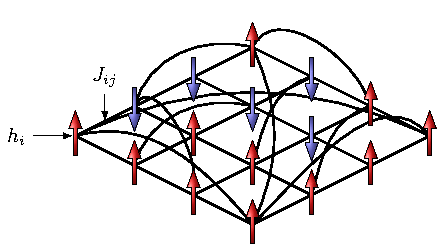
\includegraphics{figures/spins.pdf}
    \caption{Symbolic representation of Ising spin--glass defined on the graph with $N=16$ nodes. Here, $h_i$ is a real number associated with $i$-th node, and $J_{ij}$ denotes coupling strength associated with an edge between $i$-th and $j$-th node. The configuration of each spin is marked by a red arrow pointing upwards (+1) or a blue arrow pointing downwards (-1).}
    \label{fig:my_label}
\end{figure}

\begin{example}
Consider an Ising model instance with 3 spins given by the Hamiltonian $H$:
\begin{equation}
H(s_1, s_2, s_3) = s_1 - s_2 +2s_3 - 2s_2s_3 + 3s_1s_2
\end{equation}
This instance has 8 possible states:

\begin{table}[h]
    \begin{center}
        \begin{tabular}{|c|c||c|c|}
        \hline
        $\mathbf{s}=(s_1, s_2, s_3)$ &
        $H(\mathbf{s})$ &
        $\mathbf{s}=(s_1, s_2, s_3)$ &
        $H(\mathbf{s})$\\\hline
        (-1, -1, -1) & -1 & (1, -1, -1) & -5\\ \hline
        (-1, -1, 1) & 7 & (1, -1, 1) & 3 \\ \hline
        (-1, 1, -1) & -5 & (1, 1, -1) & 3 \\ \hline
        (-1, 1, 1) & -5 & (1, 1, 1) & 3\\ \hline
        \end{tabular}
    \end{center}
\end{table}
Observe that the lowest attainable energy is -5 and there are 3 states with this energy (we call
this situation a \emph{degeneracy}). Hence, all the configurations $(-1, 1, -1), (-1, 1, 1), (1,
-1, -1)$ are ground states. For this instance, a low energy spectrum of size $k=5$ comprises all
ground states, the $(-1, -1, -1)$ state with $H(-1, -1, -1) = -1$ and any of the states with
$H(\mathbf{s})=3$.
\end{example}

Despite the simple formulation, the problem of finding a ground state of Ising spin--glass is
computationally hard \cite{barahoma}. Before expanding on this idea, let us first introduce the
hierarchy of complexity classes.

\section{Algorithms and complexity}


Solving the computational problem requires a suitable \emph{algorithm}, a description of steps to be
performed by a computer to obtain a solution. It is hardly surprising that some problems might be
solved in more than one way, i.e. there might exist different algorithms performing essentially the
same task. Different algorithms solving the same problems might vastly differ in their demand on
various resources, like memory or time needed to execute them. In practice, execution time (and
usage of other resources) of a given algorithm might also vary between its implementations,
depending on factors like programming language or libraries used and the hardware it is executed on.
Therefore, measuring execution time is not that useful in characterizing the algorithm's
performance.  Instead, it is more useful to characterize algorithms based on how their execution
time scales (asymptotically) with increasing problem size\cite{arora}. For instance, given an
algorithm with execution time roughly proportional to the input size $N$, one might suspect that for
problem instances large enough, it will perform better than the one with execution time proportional
to $N^{2}$. This characteristic, known as computational complexity\footnote{Note that here we focus
only on \emph{time complexity}, but other notions like memory complexity can be defined similarly},
can be formalized by a big-$O$ notation (see appendix for more detailed description). Using this
notation, the algorithms from the above example would be classified as $O(N)$ and, $O(N^{2})$
respectively.

\section{Complexity classes}
Although there might exist multiple algorithms for solving a given computational problem, one might
consider the minimal time complexity required to do so. More generally, one might group
computational problems based on their demand on resources. In this view, sets of similar problems
are called \emph{complexity classes} \cite{arora}. The definition of some complexity classes might
also be restricted to specific types of problems. For instance, one might consider only decision
problems \cite{arora}, i.e. problems to which the answer is yes or no.

One of the fundamental complexity classes is \textbf{P}, a class of decision problems solvable in polynomial time on a deterministic Turing Machine  \cite{arora}. Another class, \textbf{NP}, comprises all decision problems whose solution can be verified in polynomial time using a deterministic Turing Machine \cite{arora}.
One can immediately see that \textbf{P} $\subset$ \textbf{NP}. Indeed, if a problem is solvable in polynomial time, then it is also trivially verifiable in polynomial time. However, it is not immediately obvious if the inclusion is strict, and whether \textbf{P} $\ne$ \textbf{NP} is one of the most important, yet unsolved problems in theoretical computer science \cite{fortnow}.
The class of \textbf{NP--hard} problems comprises all the problems that are at least as hard as
every problem in \textbf{NP}. More formally, given decision problem P is \textbf{NP--hard} if and
only if solving every problem in \textbf{NP} can be reduced to solving P a polynomial number of times
\cite{arora}. A particular subclass of \textbf{NP--hard} problems, \textbf{NP--complete}, is an
intersection of \textbf{NP} and \textbf{NP--hard} \cite{arora}. Figure \ref{fig:complexity} shows
the relationship between the discussed complexity classes, both under assumptions \textbf{P} =
\textbf{NP} and \textbf{P} $\ne$ \textbf{NP}.

Problems in the complexity class \textbf{P} are often considered tractable, or efficiently solvable,
whereas problems not in \textbf{P} are perceived as hard and computationally demanding, a statement
known as the Cobham's thesis \cite{cobham, arora}. At first, one might find it strange and
unintuitive. After all, a decision problem for which the best known algorithm runs in $O(N^{10^5})$
time is definitely in  \textbf{P}, but can hardly be called efficiently solvable. However, such
large polynomial complexities are rarely encountered in practice. Furthermore, even in such cases,
it is not uncommon that a better algorithm (e.g. with complexity $O(N^5)$) is found shortly after
the original one is discovered \cite{arora}.

\begin{figure}
    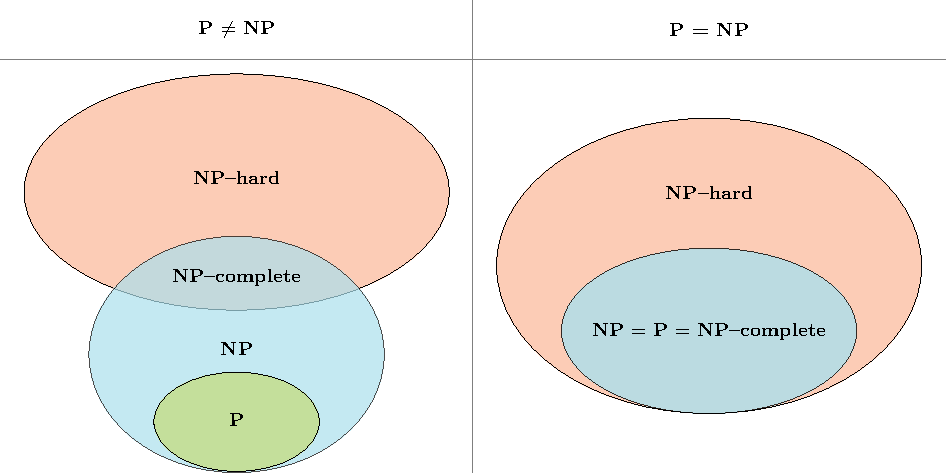
\includegraphics[width=\textwidth]{figures/complexity_new.pdf}
    \caption{Hierarchy of basic complexity classes. Under the assumption of $\textbf{P} \ne \textbf{NP}$ (left), the hierarchy is richer and there exist problems in \textbf{NP}  that are not \textbf{NP}--complete. Under the opposite assumption (right), the hierarchy collapses. Notice that in both cases there exist \textbf{NP}--hard problems that are not in \textbf{NP}
    }
    \label{fig:complexity}
\end{figure}



\section{Ising model and complexity}

Thus far, we only discussed classes of decision problems. How do they relate to the problem of
finding a ground state of the Ising model? Suppose we are given an Ising model instance with
hamiltonian $H$ and let $x \in \RR$ be some fixed number. Consider the problem of deciding whether
there exists $\mathbf{s}$ such that $H(\mathbf{s}) \le x$. We will call this problem a
\emph{decision version of the Ising problem}.

If we can minimize $H$, we can also solve the decision problem by simply finding a ground state and
checking if its energy exceeds threshold $x$. On the other hand, the sole capability of solving the
decision version of a problem does not give us an algorithm for solving an original optimization
problem. Therefore, one can see that the optimization problem is at least as hard as the
corresponding decision problem. Of course, the same reasoning applies for other optimization
problems. Hence, if the decision version of an optimization problem is \textbf{NP--hard},
the optimization problem is sometimes also called \textbf{NP--hard}, even if it slightly abuses the
notation. For simplifying the vocabulary, in what follows we will use this slightly
incorrect but more concise convention.

One can immediately see, that the state space of the Ising model with $N$ spins comprises $2^{N}$
different configurations. It might be tempting to reason that a problem with such an enormous number
of possible solutions must be \textbf{NP--hard}. While this is indeed the case, the size of the
solution space itself is not enough to reason about the problem's hardness\footnote{For instance,
the number of possible spanning trees in the complete graph of $N$ vertices is $N^{(N-2)}$, yet the
minimum spanning tree problem is solvable in polynomial time via several algorithms \cite{clrs}}.
It was shown that finding a ground state of the Ising spin--glass in the case of three-dimensional
lattices, as well as for some planar graphs,  is \textbf{NP--hard} \cite{barahoma}. The decision
version of the problem is \textbf{NP--complete}. Multiple known \textbf{NP--hard} problems, such as
Travelling Salesman Problem or Hamiltonian Cycles Problem, are reducible to finding the ground state of Ising spin-glass \cite{lucas}.

\section{Algorithms for solving Ising model}

\begin{figure}
    \centering
    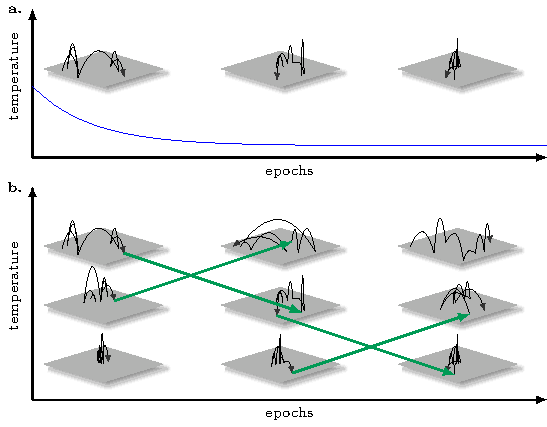
\includegraphics[width=\textwidth]{figures/pt_and_sa.pdf}
    \caption{Schematic representation of simulated annealing \textbf{(a)} and parallel tempering \textbf{(b)} algorithms. In simulated annealing, a single copy of the system is simulated. The temperature of the system is decreasing with each epoch, thus reducing movement through the state space. In parallel tempering, several copies (replicas) of the system are simulated, each with a fixed temperature. Hotter replicas move through the state space rapidly and less predictably, while colder replicas move conservatively. Between epochs, replicas can exchange states, which helps avoid being stuck at local minima. Exchanging replicas can also be viewed as reseeding of the colder replicas by randomized solutions provided by hotter replicas.}
    \label{fig:sa}
\end{figure}


As is the case with many \textbf{NP--hard} optimization problems, there are many heuristic
approaches for solving the Ising model. One family of such algorithms relies on the Metropolis-Hastings
\cite{beichl} algorithm for sampling from the underlying Boltzmann distribution. In simulated annealing
\cite{cook, isakov}, one lowers the temperature over time. Thus, the chance of accepting a locally
worse solution is greater at the start of the algorithm and decreases with each iteration, which
helps avoid getting stuck in a local minimum. In another approach from the same family,
\emph{parallel tempering}, one simulates several replicas of the system, each of them in a different
temperature. Neighboring replicas are allowed to exchange states, with exchange probability
depending on their energy and temperature difference \cite{swendsen}. Replicas with higher
temperatures explore state space rapidly (thus reseeding the algorithm), while ones with lower
temperatures refine the best solutions found so far. Various modifications of the aforementioned
algorithms exist. For instance, one could employ isoenergetic cluster moves \cite{zhu} or adaptive
choosing the number of sweeps performed between replica exchanges \cite{bittner}. Population
annealing is another Monte Carlo method, sharing similarities with simulated annealing and parallel
tempering \cite{wang}. Other approaches for solving Ising spin--glasses include methods involving
branch--and--bound framework \cite{rendl}, its chordal extensions \cite{baccari} or methods based on
simulating dynamical systems \cite{sheldon}.
%%% Local Variables:
%%% mode: latex
%%% TeX-master: "../main"
%%% End:

\chapter{Technologies involved}
\label{chapter:near-term}

 In this chapter we discuss technologies used for performing research presented in this work.
 First, we discuss quantum annealing, a quantum computation paradigm witnessing rapid development in recent years. The second discussed technology, Nvidia CUDA, is present on the market for well over a decade, yet each and every iteration of GPUs brings to the table new functionalities and performance improvements. 


\section{Adiabatic quantum computation and quantum annealing}
One of the possible alternatives to the standard gate model is adiabatic quantum computation which relies on adiabatic quantum theorem \cite{born}. Informally, the theorem states that if the physical system starting from its instantenous ground state is driven slowly enough, the evolution follows hamiltonian and the system stays in the instantenous ground state. Adiabatic quantum computing might be realized in a form of quantum annealing. In this metaheuristics, a goal is to minimize value of some target function $f$. In order to do so, one first has to find some Ising hamiltonian $H$ whose ground state encodes the optimal solution to the problem. Then, the system is prepared in a ground state of some initial, simpler hamiltonian $H_0$. After that. The system is slowly perturbed in such a way that its hamiltonian changes from $H_0$ to $H$, i.e. the evolution of the system is governed by the following hamiltonian $H_\text{total}$
\begin{equation}
    \label{eq:aqc}
    {H}_\text{total}(s) = a(s) {H}_0 + b(s){H}, \quad s \in [0, \tau]
\end{equation}
where $a(\tau) = b(0) = 0, \; a(0) = b(\tau) = 1$, and $a$ and $b$ are decreasing and increasing functions respectively.
By adiabatic quantum theorem, if the evolution described by the equation \eqref{eq:aqc} is slow enough, the system will stay in ground state of ${H}_\text{total}(s)$ for every $s \in [0, \tau]$. In particular, after reaching $s=\tau$, i.e. when $H_\text{total} = H$, the state of the system should encode an optimal solution to target optimization problem.

\subsection{Comparison to classical model of computation}
It is clearly visible that quantum annealing is different from computing using classical computers. One of the most obvious differences is computational model. On classical computers one essentially writes programs as a series of instructions to be executed by the CPU. On typical machines, CPU is capable of performing arithmetic operations, computing values of some special functions, managing execution flow, controlling I/O and much more. In comparison, quantum annealers are capable of executing a single operation: annealing given optimization problem. Therefore, programming these devices boils down to defining optimization problem and tuning the annealing parameters. There is no processing flow controlled by the programmer.

Another difference between classical computers and quantum annealers is lack of working memory in the former. Classical computers use working memory (typically in the form of RAM) to store machine code and data. However, quantum annealers do not need to store neither code or data, and hence they do not feature analogous component. Similarly, quantum annealers, being purely computational oriented devices, do not have mass storage.

A slightly less obvious difference between classical computers and quantum annealers is their model of parallelism. Classical computers are capable of running several threads of execution at the same time. However, every nontrivial classical algorithm involving parallelism must necessarily also include a serial part, which limits speedup gained for introducing more CPU cores or CPUs. In contrast, quantum annealers are capable of annealing multiple qubits at the same time, which makes their operation inherently parallel.

\subsection{D-Wave quantum annealers}

The first commercially available quantum annealer was introduced by D-Wave company in 2011. At the time of writing, the newest series of D-Wave annealers is The Advantage System utilizing chip with at least 5000 qubits. These novel devices deomnstrate a significant improvement over previous 2000Q generation, which used at most 2048 qubit chip with sparser connectivity. Since most research utilizing quantum annealers in this work was conducted using 2000Q devices, in what follows we mostly limit our attention to this specific devices.

\begin{figure}[h]
    \centering
    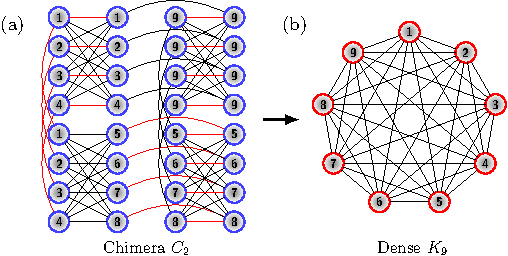
\includegraphics[width=\textwidth]{figures/chimera.pdf}
    \caption{\textbf{a.} Example of Chimera topology. Graph presented here consists of $2 \times 2$ grid of unit cells (hence $C_2$ name). Note the sparse connectivity of the presented graph as compared to the full graph with the same number of nodes. \textbf{b.} Full $K_9$ graph embedded in Chimera graph from \textbf{a.}. The nodes are labelled with numbers corresponding to groups of logical qubits they were constructed from.}
    \label{fig:chimera}
\end{figure}


\subsection{Annealer topologies}

The Ising model described in previous chapter allows arbitrary interactions between spins. However, this is often not the case with physical devices like quantum annealers. For instance, in D-Wave devices spins are arranged into a specific \emph{topology} with limited connectivity. Thus, the possible graph on which the optimization problems can be defined is much sparser than the complete $K_{N}$ graph. Spins in 2000Q devices are arranged in the so called \emph{Chimera} topology depicted in figure \ref{fig:chimera}. The Chimera graph can be thought of as a $n \times m$ lattice of unit cells, where each cell is a complete bipartite $K_{4,4}$. Qubits are also connected to two qubits in neighbouring cells via external couplers (unless they reside on the border or a corner of the lattice), resulting in at most total 6 connections per qubit. Straightforward calculation shows that Chimera graph has total of $16mn + 4(m-1)n + 4(n-1)m$ edges.

The new Advantage system uses \emph{Pegasus} topology, which increases maximum degree of vertex in the graph to 15. For the details of this topology we refer interested reader to \cite{boothby}.

\subsection{Minor embeddings}
Not every Ising problem one might wish to solve is compatible with topology of physical quantum annealer. This issue can sometimes be circumvented using procedure called \emph{minor embedding}. In this approach one considers groups of several physical spins connected in a chain as a single logical one. Vertices corresponding to spins in each such chain are contracted, resulting in the new graph, having higher connectivity but smaller number of vertices than the original one. With the proper choice of chains this new graph can contain a subgraph isomorphic to the graph of the problem to solve. The minor embedding process is illustrated in figure \ref{fig:chimera}.

Grouping qubits into chains and contracting them is not enough to run the embedded problem. One first has to ensure that all spins in a chain align in the same direction, so that they can indeed represent a single logical variable. This is accomplished by adding a penalty term which prohibitively increases cost of solutions in which value of spins in chains differ. However, due to the probabilitsic nature of quantum annealer, even after adding penalty one might obtain solutions in which values of spins in some chains disagree. Such disagreeing chains are called \emph{broken}. Since solutions containing broken chains cannot be interpreted directly as a solution to the original problem, one has to either discard them, or manually correct them (e.g. by choosing most common value among the spins in chain).

% To define minor embedding more formally, let us first define the notion of vertex contraction. Let $(G, E)$ be a graph defining topology of the device and let $v_{1}, \ldots, v_{{n}} \in E$ be a chain of vertices. Contraction of vertices $v_{1}, \ldots, v_{n}$ is a new graph $G'=(V', E')$ such that
% \begin{itemize}
%   \item $V' = V \setminus \{v_{1}, \ldots, v_{{n}}\} \cup \{w\}$, where $w$ is some new vertex.
%   \item $E' = \{e \in E\colon v_{i} \notin E\} \cup \{\{v, w\}\colon \exists_{i} \{v, v_{i}\} \in E\}$
% \end{itemize}
% Intuitively, contracting vertices replaces them with a new one connected with their every neighbour.

\section{Nvidia CUDA}

Quantum annealing, introduced in the previous section, is an inherently heuristic process. Like many heuristic algorithms, it cannot certify that the solution it found is in fact optimal. One way to assess performance of such algorithms is to compare their results with known low-energy spectrum of some test instances. In this section, we describe the Nvidia CUDA technology, which we use for our implementation of massively parallel brute-force algorithm describe in chapter \ref{chapter:bruteforce}.

\subsection{Brief history of Graphics Processing Units}
History of specialized hardware for manipulating graphics ranges as far as to 1970s. Initially these devices, that later became known as Graphics Processing Units (GPU), offered limited functionalities. Increasing demand for performance in gaming industry and professional graphics processing drove the evolution of GPUs, which quickly became highly sophisticated devices supporting advanced 2D and 3D image manipulation. Performing such arithmetically intensive operations requires enormous computational power, and it was only the matter of time until it was realised that the power of these devices can be harnessed for general purpose computations (so called GPGPU - General Purpose computing on GPU). 

Early efforts in development of GPGPU required framing of computational problem in terms of operations performed on graphical primitives, as this was the only way for using specialized API of GPUs. This changed with the development of devices and toolkits that supported operations needed for general purpose computations out of the box. Notably, in 2007 Nvidia introduced its massively parallel CUDA architecture.

\subsection{Differences between CPU and GPU}
Principles behind operation of CUDA-enabled devices are fundamentally different than the ones governing execution of program on traditional CPU-only architecture. In current x86 based computers, CPU runs given sequence of instructions (so called thread of execution) using one of its cores. Such processor is the ''brain'' of a computer, and it can perform a wide variety of tasks ranging from arithmetic operations, through accessing system's RAM, to performing IO operations and controlling other components of the system. Typical CPUs are optimized for sequential execution, and as such are usually equipped with moderate (as compared to the GPUs) number of high-performance cores. 

On the other hand, GPUs are more specialized. They are well suited for performing a large number of arithmetic operations and accessing memory in parallel. They typically have more cores than a traditional CPU (with even modern commodity GPUs boasting thousands of them). Although those cores are less performant than their CPU counterparts and support much narrower set of operations, their large number combined with fast memory access gives modern GPUs advantage over CPUs in multiple areas.

\subsection{Processing flow on CUDA}
Considering the architectural differences between CPUs and GPUs, it is hardly surprising that both of these types of devices are programmed quite differently. The first major difference is that GPUs cannot operate on their own and are themselves controlled by CPU. This is why CUDA is a type of \emph{heterogenous} architectures (as opposed to CPU-only \emph{homogenous} architectures). The processing flow on CUDA is summarized in Figure \ref{fig:cuda_flow}.

\begin{figure}[ht]
    \centering
    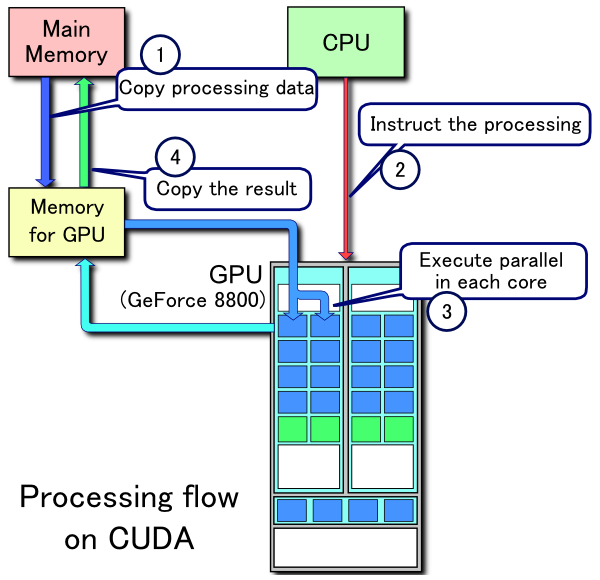
\includegraphics[width=0.7\textwidth]{figures/CUDA_processing_flow_(En).png}
    \caption{{\protect\todo[inline]{Important: this figure is only here temporarily, I will prepare my own graph once the text is done.}} Processing flow on CUDA. The CPU sends input data to the GPU memory, and launches the computational kernel. The kernel's code is executed, in parallel, using multiple threads on GPU. Once the execution is done, results are copied from the GPU memory to the system's RAM.}
    \label{fig:cuda_flow}
\end{figure}

Programs run on GPU are organized in \emph{kernels}. For the most part kernels might be viewed as functions or subroutines (which is indeed how they are implemented) that don't have a return value. On a CPU, such function would be executed by some core as a part of a thread. In CUDA however, the very same kernel is executed by multiple threads. Executing a kernel requires specifying a \emph{grid} that will be used for running it. A grid can be 1, 2 or 3 dimensional and is itself divided into blocks. Each block is in turn also organized in 1, 2, or 3 dimensional structure of threads (the same for every block in the grid). Schematic view of a two-dimensional grid is presented on Figure \ref{fig:cuda_grid}.

\begin{figure}[ht]
    \centering
    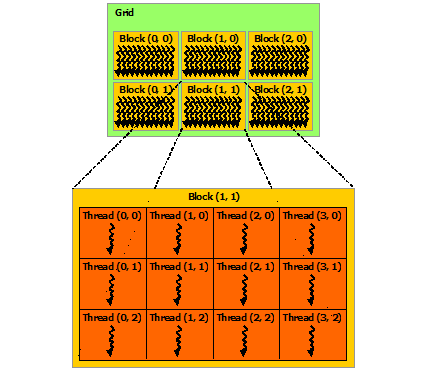
\includegraphics[width=0.8\textwidth]{figures/grid-of-thread-blocks.png}
    \caption{{\protect \todo[inline]{This is also a temporary figure...}} A schematic view of an example two-dimensional CUDA grid. Presented here is a 2 $\times$ 3 grid of 3 $\times$ 4 blocks.}
    \label{fig:cuda_grid}
\end{figure}

As already mentioned, each thread in the grid executes \emph{precisely the same} kernel. It might therefore seem surprising that nevertheless they are able to access different parts of memory. This is possible, because each thread is identified by its indices in both the grid and the block. Those indices can be used e.g. for computing offsets in arrays that are being processed. A more sophisticated use of thread and block indices will be exemplified in chapter \ref{chapter:bruteforce}.

\subsection{SIMT architecture}
CUDA-enabled GPUs employ architecture called SIMT (Single Instruction, Multiple Threads)\footnote{One can contrast SIMT architecture used by CUDA with SIMD instructions (Single Instruction, Multiple  Data) available on mother CPUs.}. As implied by the name, in SIMT architecture multiple threads execute the therey same instruction. Threads are executed in blocks  by computational units called Streaming Multiprocessors (SMs), and blocks distributed to multiprocessors on kernel launch. When a block is distributed to SM, it is further partitioned into \emph{warps}, groups of 32 threads each. All threads in a warp are scheduled for execution together. Nevertheless, they have separate program counter and thus their execution flow can diverge. At any given time a  thread in a warp can be either active (executing \emph{the same} instruction as the rest of the active threads in a warp) or inactive (not executing any instruction at all). Thread may be inactive because its execution diverged from the rest of the warp or because it terminated earlier. It is interesting to note that starting from the Volta architecture threads can be scheduled on finer level of granurality, allowing them to diverge and reconverge on the sub-warp level. Each multiprocessor manages set of 32-bit registers and parallel data cache, called \emph{shared memory} distributed among the thread blocks. Since those resources are limited, the number of warps that can run in parallel on any SM is heavily dependent on resource usage of the kernel being executed.

\subsection{Memory hierarchy}

Threads can access several memory types during kernel execution, including global memory, local memory, constant and texture memory and shared memory. Physically, those different memory types can be divided into device memory (global memory, local memory, constant memory) and on-chip memory (shared memory). SM's on-chip memory also serves as L1 cache.

Global memory is a device memory available to each thread. All accesses to global memory are serviced in 32-, 64-, or 128- bytes memory transactions. Accesses made from a single warp are coalesced into as many of such transactions as necessery, depending on device's compute capability and access pattern. Reads and writes targeting global memory are always cached in L2 and (depending on configuration, compute capability and access pattern) may also be cached in L1 cache.

Local memory resides physically on the device, and thus offers the same bandwidth and latency. Just like global memory it is always cached in L2 cache. This type oif memory is never used directly by the programmer. Instead, compiler might decide to use it for local variables of a thread in case there is not enough registers (so called \emph{register spilling}) or for dynamically indexed local arrays. Local memory is arranged in such a way, that accesses are always fully coalesced as long as all threads access the same relative address (e.g. the same local variable, the same index of local array etc.).

Constant memory and texture memory are two types of read-only memory \footnote{Read-only here means ``Not writeable from inside the kernel''} residing in global memory. Accesses to constant memory are cached in constant cache and accesses to it are serialized. Therefore, each request is split into as many  transactions as there are different memory addresses in the original request. Texture memory is cached in texture cache, which is optimized for accessing spatial data. Hence, the best performance is achieved if threads in a warp read or write to the addresses that are close in 2D.

Threads can cooperate and share data through the use of on-chip \emph{shared  memory}. The amount of allocated shared memory is directly controlled by the programmer either on the kernel definition level, or during its launch. Shared memory is organized in banks that can be accessed simultanenously, and the best performance is achieved if each thread in a warp accesses memory in a different bank. Otherwise, a \emph{bank conflict occurs} and the request is split into as little conflict-free requests as possible.


\subsection{Programming environment}
CUDA devices can be programmed directly using either C/C++ or Fortran. The C/C++ code can be compiled using Nvidia's nvcc compiler, shipped out of the box with CUDA toolkit, while using Fortran requires installing its third-party distribution (e.g. PG Fortran developed by Portland Group). Giving a comprehensive walkthrough of using either C/C++ or Fortran with CUDA is well beyond the scope of this thesis, but for the sake of completeness we present a short example of CUDA Fortran code in listing \ref{lst:cuda_fortran} \todo{Note to self: remember to either replace it with my own example or cite the source (CUDA Fortran documentatoin)}.

\begin{lstlisting}[
    language=Fortran,
    label=lst:cuda_fortran,
    captionpos=b,
    caption={Example code in CUDA Fortran. Presented here are an example kernel performing saxpy operation together with a host subroutine that uses it.},
    frame=tlrb,
    aboveskip=2em,
    belowskip=2em
]{fortran}
! Kernel definition
attributes(global) subroutine ksaxpy( n, a, x, y )
   real, dimension(*) :: x,y
   real, value :: a
   integer, value :: n, i
   i = (blockidx%x-1) * blockdim%x + threadidx%x
   if( i <= n ) y(i) = a * x(i) + y(i)
end subroutine

! Host subroutine
subroutine solve( n, a, x, y )
   real, device, dimension(*) :: x, y
   real :: a
   integer :: n
   ! call the kernel
   call ksaxpy<<<n/64, 64>>>( n, a, x, y )
end subroutine
\end{lstlisting}

Along the nvcc compiler, the CUDA toolkit contains several, more specialized libraries. Among others, those include:
\begin{itemize}
    \item cuBLAS -- CUDA Basic Linear Algebra Subroutines library,
    \item cuFFT -- CUDA Fast Fourier Transform library,
    \item cuRAND -- CUDA Random Number Generation library,
    \item cuSPARSE -- CUDA library for manipulating sparse matrices.
\end{itemize}
For many high-level languages, there exist third-party wrappers enabling use of CUDA (e.g. PyCuda for Python).



%%% Local Variables:
%%% mode: latex
%%% TeX-master: "../main"
%%% End:

\chapter{Simulating dynamics of quantum systems using quantum annealing}
\chaptermark{Simulating dynamics}
\label{chapter:simulating}

One of the leading motivations behind the development of quantum computing
devices is simulating quantum systems intractable by classical computers. But
how far are we from this goal? To answer this question, one might design an
algorithm for conducting such a simulation of a physical system and then test
how it performs on the current generation of quantum computers. In this
chapter, we follow this idea and present a possible approach for simulating
quantum systems (or any time-dependent dynamical system) that can be used with
annealing devices such as D-Wave quantum annealers and similar devices. To
illustrate the working of our algorithm, we simulate the simplest single-qubit
system and demonstrate that already near-term annealing devices are capable of
capturing its dynamics in a narrow regime of parameters. Furthermore, the class
of physics-inspired instances of the Ising model proposed in this chapter
can be valuable in benchmarking other (not necessarily quantum) solvers.

\section{Parallel in time simulation of dynamical systems}
Optimization problems that can be solved using quantum annealers exhibit no
time--dependence. Therefore, simulating any time-dependent phenomena using
those devices requires reformulating the problem as one that is static in
nature. In our case, it is possible by enlarging the Hilbert space of the
system under consideration, so that the states of this larger space encode also
temporal information \cite{feynmanclock}.

Let us first start by precisely defining the problem we want to address.
Consider an $L$--dimensional real or complex system, whose state at time $t$ is
described by the vector $\ket{\psi(t)}$ evolving according to a differential
equation of the form
\begin{equation}
  \label{eq:dynamical-system}
  \frac{\partial \ket{\psi(t)}}{\partial t} = K(t) \ket{\psi(t)}.
\end{equation}

Here, $K$ is the so-called Kamiltonian \cite{goldstein2002classical} and can be
any linear operator acting on $\mathbb{R}^L$ or resp. $\mathbb{C}^L$. Observe
that any isolated quantum system can be described by equation
\eqref{eq:dynamical-system}, as putting $K=-\frac{i}{\hbar}H$, where $H$ is its
Hamiltonian, transforms the equation \eqref{eq:dynamical-system} into
Schr\"{o}dinger equation.

Given an initial state, $\ket{\psi(t_0)}$ the equation
\eqref{eq:dynamical-system} admits a unique solution, namely
\begin{equation}
  \ket{\psi(t)} \coloneqq U(t, t_0) \ket{\psi(t_0)},
\end{equation}
where operator $U(t, t_0)$ is a propagator transforming the initial state of
the system into its state at time $t$ and is given by
\begin{equation}
  \label{eq:propagator}
  U(t, t_0) = \mathcal{T} \exp \left( \int_{t_0}^t K(\tau)d\tau \right).
\end{equation}
Here, $\mathcal{T}$ denotes the time-ordering operation \cite{chronological}.
Note that in the case when $K(t)$ commutes with $K(t')$ for every $t' \ne t$,
the time-ordering can be omitted. In particular, this is the case if $K$ is
time-independent.

Given the initial state, we are interested in finding the state of the system
at some time $t > t_0$. Numerical methods for solving this problem usually
start by partitioning the interval $[t_0, t]$ into $N$ distinct time points
$t_0 < t_1 < \ldots < t_{N-1} = t$. Then, the desired state $\ket{\psi(t)}$ can
be computed as
%
\begin{equation}
  \ket{\psi(t)} = U_{N-1} \cdots U_1 \ket{\psi(t_0)},
\end{equation}
%
where $U_i$ is a shorthand notation for $U(t_i, t_{i-1})$. This is purely a
rearrangement of computations, which by itself gives no benefit over applying
$U(t, t_0)$ directly. However, shortening the interval allows for a more
efficient approximation of propagators, which can be done using a variety of
methods, including Suzuki-Trotter approximation \cite{suzuki}, commutator-free
expansion \cite{commutatorfree} or tensor-networks based approaches
\cite{dmrg}.

This procedure, common to many sequential methods, gives a starting point for a
class of the so-called parallel in--time methods based on the Feynman clock
operator. In these approaches, one starts by suitably enlarging the state space
so that it can encode the temporal data \cite{feynmanclock}. This can be done
by considering a tensor product of a state space with the new Hilbert space
spanned by the orthonormal basis $\{\ket{0}, \ket{1}, \ldots, \ket{N-1}\}$.
Then, the following superposition encodes states of the system in all $N$
moments of time
%
\begin{equation}
  \ket{\Psi} = \sum_{n=0}^{N-1} \ket{n} \otimes \ket{\psi(t_n)}.
\end{equation}
Consider now the following \emph{clock operator} $\clockop$
\begin{equation}
  \label{eq:clock2}
  \begin{split}
    \clockop
    =
    \sum_{n=0}^{N-2}
    &\ketbra{n+1}{n+1} \otimes I - \ketbra{n+1}{n} \otimes U_n + \\
    &\ketbra{n}{n} \otimes I - \ketbra{n}{n+1}\otimes U_{n}^{\dagger}.
  \end{split}
\end{equation}
One can see that $\ket{\Psi}$ is a solution (although not unique) to the
eigenequation
\begin{equation}
  \label{eq:clock-eigenequation}
  \clockop \ket{\mathbf{x}} = 0.
\end{equation}
The non--uniqueness of the solution of \eqref{eq:clock-eigenequation} follows
from the fact that the definition of the clock operator $\clockop$ does not
depend on the initial state. We can fix this problem by adding a \emph{penalty}
term $\clockop_0 = \ketbra{0}{0}\otimes(I-\ketbra{\psi_0}{\psi_0})$ to the
left-hand side. The equation to solve becomes then:
\begin{equation}
  \label{eq:clock-eigenequation2}
  (\clockop + \clockop_0) \ket{\mathbf{x}} = 0.
\end{equation}
If one puts $\coefmatrix=\clockop + \ketbra{0}{0} \otimes I$ and $\ket{\Phi} =
  \ket{0}\otimes \ket{\psi_0}$, the equation \eqref{eq:clock-eigenequation2}
becomes:
\begin{equation}
  \label{eq:gsys}
  \coefmatrix \mathbf{x} = \ket{\Phi}.
\end{equation}
Thus, using an approximation of evolution operators, we constructed a system of
linear equations encoding the solution to the equation
\eqref{eq:dynamical-system} under the given initial condition. At this point,
however, it is not possible to solve it using a quantum annealer yet. To do so,
one first needs to convert this system into an optimization problem with
dichotomous variables, which is what we will deal with next.
\section{Solving systems of linear equations as an optimization problem}
There is a straightforward way of converting equation \eqref{eq:gsys} into an
optimization problem. One can observe that the solution minimizes the norm
$\left\Vert \coefmatrix\ket{\mathbf{x}} - \ket{\Phi}\right\Vert$. Since the
norm is non-negative, it follows that solving equation \eqref{eq:gsys} is
equivalent to the following optimization problem
\begin{equation}
  \label{eq:optimize_1}
  \ket{\Psi} = \argmin_{\mathbf{x}} f(\mathbf{x}), \quad f({\mathbf x}) = \left\Vert \coefmatrix\ket{\mathbf{x}} - \ket{\Phi}\right\Vert^2.
\end{equation}
However, $f$ in the equation \eqref{eq:optimize_1} is not the only choice of a
target function. If $\coefmatrix$ is positive-definite, one can consider the
following function $h$ instead
\begin{equation}
  \label{eq:optimize_2}
  h(\mathbf{x})=\frac{1}{2}\bra{\mathbf{x}}\coefmatrix\ket{\mathbf{x}} -
  \braket{\mathbf{x}}{\Phi}.
\end{equation}
Indeed, one can verify that solution to \eqref{eq:gsys} also minimizes $h$ by
computing its gradient and Hessian
\begin{equation}
  \nabla h(\mathbf{x}) = \coefmatrix\ket{\mathbf{x}}-\ket{\Phi}, \quad \nabla^2 h({\mathbf
    x})=\coefmatrix>0
\end{equation}
Since Hessian is positive and $\ket{\Psi}$ is the only vector at which $\nabla
  h$ vanishes, it follows that $\ket{\Psi}$ is indeed a global minimum of $h$.

\section{Discretizing variables}
Thus far, we have been working with continuous variables. The next necessary
step before solving optimization problems \eqref{eq:optimize_1} and
\eqref{eq:optimize_2} using annealer is converting them in such a way that all
unknowns are dichotomous. To this end, we will follow a strategy presented in
\cite{fixedpoint,chang}. The idea is to express each of the unknown
coefficients of $\ket{\mathbf{x}} = $[$x_1, \ldots, x_{LN}]^T$ in fixed-point
approximation. If one assumes (binary) order of magnitude of coefficients of
$\mathbf x$ to be $D$ (i.e. $x_i \in [-2^D, 2^D]$ for each $i$), then it can be
approximated up to $R$ bits of precision as
\begin{equation}
  \label{eq:fixed}
  x_i \approx 2^D \left(2 \sum_{\alpha=0}^{R-1}2^{-\alpha}q_i^{\alpha} -1\right).
\end{equation}
Here variables $q_i^\alpha$ are consecutive bits of the fixed-points expansion
of $x_i$. Note that approximation of $x_i$ in \eqref{eq:fixed} is a linear
combination of its bits, therefore plugging it into optimization problems
\eqref{eq:optimize_1} and \eqref{eq:optimize_2} yields quadratic unconstrained
optimization problems of the form
\begin{align}
  \label{eq:qubo_f}
  \argmin_{\mathbf{q}} f(\mathbf{q}) = \argmin_{\mathbf{q}} \sum_{i,\alpha} c_i^{\alpha} q_i^r + \sum_{i,j,\alpha,\beta} d_{ij}^{\alpha\beta} q_i^{\alpha} q_j^{\beta} + f_0, \\
  \label{eq:qubo_h}
  \argmin_{\mathbf{q}} h(\mathbf{q}) = \argmin_{\mathbf{q}} \sum_{i,\alpha} a_i^{\alpha} q_i^r + \sum_{i,j,\alpha,\beta} b_{ij}^{\alpha\beta} q_i^{\alpha} q_j^{\beta} + h_0.
\end{align}
Coefficients in equations \eqref{eq:qubo_f} and \eqref{eq:qubo_h} can be
straightforwardly computed by appropriate substitutions into equations
\eqref{eq:optimize_1} and \eqref{eq:optimize_2}. For brevity, here we present
only the formulas for the equation \eqref{eq:qubo_h}, which reads
\begin{eqnarray}
  \begin{split}
    b_{ij}^{\alpha\beta} &= \coefmatrix_{ij} 2^{1-\alpha-\beta+2D} \\
    a_i^\alpha &= \left( 2^{-\alpha+D}\coefmatrix_{ii} - 2^D\sum_{j}\coefmatrix_{ij}- \Phi_i\right)2^{1-\alpha+D},
    \\
    h_0 &= 2^D\left( 2^{D-1}\sum_{ij}\coefmatrix_{ij}+\sum_i \Phi_i\right).
  \end{split}
  \label{eq:coeff}
\end{eqnarray}

Our approach requires the order of magnitude $D$ and precision $R$ in equation
\eqref{eq:fixed} to be chosen beforehand. Choosing the right $D$ requires
knowledge of the range in which coefficients lie. If its value is too small,
the approximations will fail to capture the most significant bits of the real
solution. On the other hand, choosing $D$ that is too large will result in
wasting variables for encoding insignificant zeros. Fortunately, for many
systems, a suitable $D$ can be determined. For instance, for qubit and
multi-qubit systems, each $x_i$ is bounded by $\pm 1$ which makes $D=0$ the
optimal choice for this case.

QUBOs in the equations \eqref{eq:qubo_f} and \eqref{eq:qubo_h} are defined on
the graph of size $N \cdot R \cdot L$. The number of edges (i.e. non-zero
quadratic terms) depends on the number of non-zero off-diagonal elements of the
matrix $\coefmatrix$. It is interesting to note that the overall density of the
graph is an increasing function of $R$ (bigger precision requires a denser
graph) while, on the other hand, it tends to decrease with increasing $L$.

We converted the original problem of finding the dynamics of the system into a
binary optimization problem suitable for input to the quantum annealer. In the
next section, we will discuss experiments that we performed using D-Wave
2000Q$_{2.1}$ and D-Wave 2000Q$_5$ machines to test the approach we described.
The results we discuss here were originally reported in \cite{parallelintime}.

\section{Parallel-in-time simulations with quantum annealer}
\sectionmark{Parallel-in-time simulations}
\label{sec:parallel-in-time}
Before discussing the results of our experiments, let us focus first on its
design. To exemplify our approach, we chose to simulate the dynamics of a
two-level system with an initial state $\ket{0}$ and a Hamiltonian
\begin{equation}
  H = \frac{\pi}{2}\sigma_y,
\end{equation}
where $\sigma_y$ is a Pauli spin operator in the $y$-direction. This particular
choice of Hamiltonian and initial state makes the system suitable for
implementation on present-day quantum annealers for several reasons. One can
easily see that the evolution of the system is real (as opposed to complex),
which halves the number of needed variables. Secondly, for integral time points
$t_0=0, t_1=1, \ldots$ coefficients of the wave function can be expressed
\emph{exactly} using only two bits of precision per coefficient, which further
reduces the number of needed variables.

\begin{figure}[!h]
  \centering
  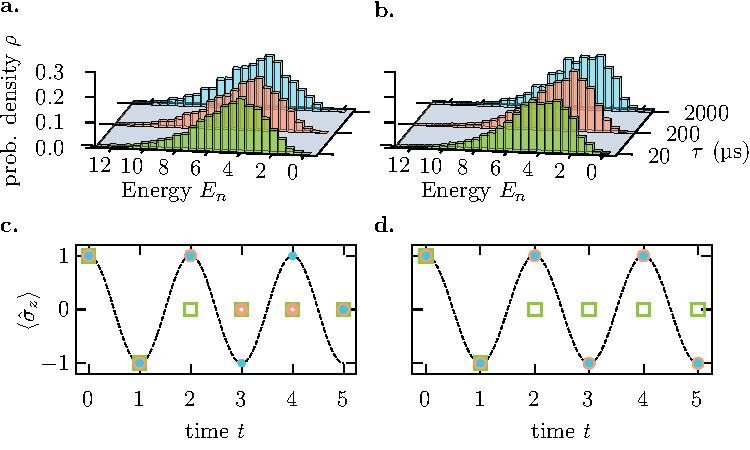
\includegraphics{figures/parallel-dynamics-result.pdf}
  \caption{Results of simulating dynamics of two-level system on D-Wave 2000Q$_{2.1}$
    (left) and low-noise D-Wave 2000Q$_{5}$ (right). \textbf{a.}--\textbf{b.}
    Energy distribution of samples obtained from D-Wave annealers for different
    annealing times $\tau$. Notice a slight shift of distributions towards the
    ground state for the 2000Q$_{5}$ device. \textbf{c.}--\textbf{d.} Rabi
    oscillations of the simulated system. The obtained samples were normed before
    plotting. As can be seen in panel \textbf{d.}, the low-noise device was able to
    faithfully capture oscillations for $\tau=200, 2000$. The annealing time is
    color-coded: $\tau=$ \tikzquad\,\,\, -- 20\textmu{}s, \,\tikzcircle\,\,\,--
    200\textmu{}s, \,\tikzdot\,\,-- 2000\textmu{}s. } \label{fig:energy-hist}
\end{figure}

We simulated the above system using values of $R=2, 3$ and for several numbers
of time points $N$. We used annealing time $\tau$ spanning several orders of
magnitude, namely $\tau=20\mu s$, $200 \mu s$ and $2000 \mu s$. Since the
resulting graphs were dense, we decided to use standard embedding of the
complete graph $K_n$ on Chimera \cite{chimeraclique}. To assess the quality of
solutions obtained from the annealer, we sampled each problem $10^4$ times on
DW-2000Q$_{2.1}$ device as well as its low-noise version, DW-2000Q$_{5}$.
Energy distributions of samples obtained for $N=6$ are depicted in Fig.
\ref{fig:energy-hist}. The same figure also illustrates the dynamics of the
expected value of $\sigma_z$ for the lowest energy sample obtained for a given
annealing time. Note that to preserve the physical meaning of the decoded
solution, the state vector was normed before plotting.

To put these results into context, we also compare them to the ones obtained
using two purely classical methods: CPLEX optimizer and recently developed
tensor network-based algorithm (which we describe later in chapter
\ref{chapter:tn}. The results of this comparison are depicted in Fig.
\ref{fig:cplex_tn_dwave}.

\begin{figure}
  \centering
  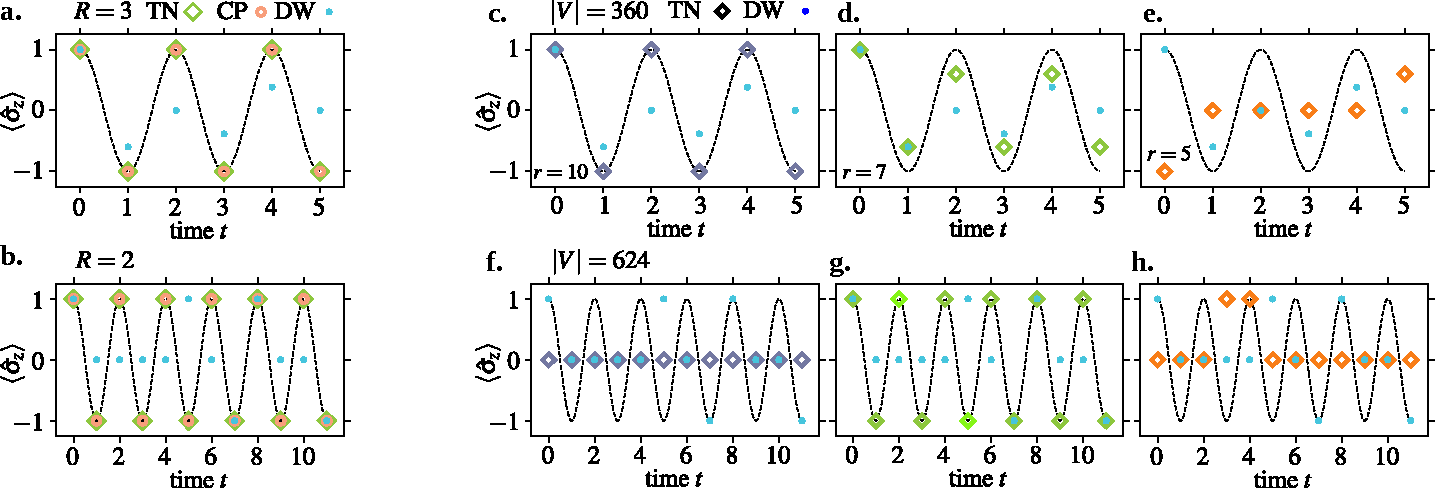
\includegraphics[width=\textwidth]{figures/fig34_merge.pdf}
  \caption{ \textbf{a.}--\textbf{b.} Performance of the two state-of-the-art heuristic
    algorithms: the CPLEX optimizer (CP) and a tensor networks-based (TN) solver
    (see chapter \ref{chapter:tn}) in comparison to the D-Wave $2000$Q quantum annealer (DW),
    cf. Fig~\ref{fig:energy-hist}. The graphs on which the problems were defined
    had respectively $|V|=360$ (\textbf{a.}) and $|V|=624$ (\textbf{b.}) vertices. The annealing time was set
    to $\tau=200$\textmu{}s. The numerical precision of the solution vector is
    denoted as $R$. %\\
    \textbf{c.}--\textbf{h.} Degradation of the solution quality resulting from perturbing the
    problem by truncating its coefficients to a given
    numerical precision denoted as $r$. The reference ground state obtained
    with tensor networks (TN) is compared to the  experimental data from the
    D-Wave $2000$Q quantum annealer (DW). This effect, expected to be predominant
    in the current quantum annealing technology, is already visible on
    Fig.~\ref{fig:energy-hist}\textbf{a.}--\textbf{d.} and Fig.~\ref{fig:cplex_tn_dwave}\textbf{a.}--\textbf{b.}.
  }
  \label{fig:cplex_tn_dwave}
\end{figure}

Results depicted in figures \ref{fig:energy-hist} and \ref{fig:cplex_tn_dwave}
show that the DW-2000Q$_{5}$ was able to faithfully capture dynamics of qubit
if the state of the system was encoded using $R=2$ bits of precision per
coefficient when the annealing time $\tau=200$ was used. For larger values of
$N$ and $R$ one can observe that the quality of solution degrades. Both CPLEX
and tensor networks-based solvers outperformed D-Wave annealers in terms of the
quality of solutions. The differences were especially noticeable for problem
instances with larger graph sizes, i.e. ones with higher precision ($R \ge 3,
  N=6)$), or with extra time points ($N > 6, R = 2$). The observed degradation of
the solution quality is consistent with the results obtained in other works,
especially for the problems requiring complete graphs, see e.g.
\cite{Hamerly2019}.

\subsection{Discussion of error sources}

The poor performance of D-Wave annealer is something certainly to be expected
from such early-stage devices. Annealers are prone to errors stemming from
multiple sources \cite{dwavedocs}, and it is hard to judge which of those
sources contributed most to the lackluster performance of a particular problem
instance. One of the possible sources of errors is DAC quantization, which
essentially limits the precision of both the quadratic and linear coefficients
passed to the annealer. As a result, the problem that the annealer physically
solves is slightly different than the problem the programmer intended to solve.

One can see that such quantization errors would mostly affect problems with
coefficients lying in close proximity to one another. Indeed, suppose that DAC
quantization errors limit the precision of the linear coefficients to $d$
decimal digits. Then any two coefficients, say $h_{i}, h_{{j}}$ lying closer to
each other than $d$, i.e. $|h_{i} - h {j}| < 10^{-d}$, become physically
undistinguishable to the annealer. The issue also affects coefficients that are
further apart, by possibly diminishing their relative differences.

While it is hard to pinpoint which source contributed the most to the errors in
the case of the optimization problems discussed in this chapter, we argue that
in our case the poor performance of the annealer can be largely explained by
DAC quantization. Indeed, looking at the \eqref{eq:coeff} one can immediately
see that the optimization problem can contain coefficients arbitrarily close to
each other as long as a large enough $R$ is chosen. To justify this reasoning,
we studied how the tensor network solver performs when the coefficients of the
problem are perturbed by truncating their coefficients to some predefined
number of digits $r$. The results of this experiment are presented in Fig
\ref{fig:cplex_tn_dwave}\textbf{(c)--(h)}. One can immediately observe that the
error patterns resemble the ones obtained from D-Wave, which might suggest that
DAC quantization might indeed be a significant source of errors in our case.
However, we would like to point out, that our analysis is by no means
conclusive, and further analysis of error patterns is still needed.

%%% Local Variables:
%%% mode: latex
%%% TeX-master: "../main"
%%% End:

\chapter{Solving spin-glass problems using tensor networks}
\label{chapter:tn}

Benchmarking quantum annealers requires more sophisticated algorithms. While
there exists a plethora of general-purpose optimization algorithms, one might
hope to achieve better results by exploiting the topology of the problem's
underlying graph and thus locality therein. In this chapter, we describe a
recent, tensor network-based algorithm for finding low-energy spectrum of Ising
spin-glasses, designed for problems defined on Chimera-like
quasi-two-dimensional graphs. The algorithm exploits the sparsity and locality
of the Chimera graph by representing the Boltzmann distribution of spin-glass
as a tensor network, whose approximate contraction can be used for computing
marginal probability distributions. This procedure can then be combined with
the well-known branch and bound algorithm to iteratively select the most
promising partial solutions, finally producing an approximation of the
low-energy spectrum.

\section{Introduction to tensor networks}

\todo[inline,color=SkyBlue]{Mention that the algorithm is physics inspired}
\todo[inline,color=SkyBlue]{Mention the other Chimera-specific algorithm}

\subsection{Branch and bound}
Let us start by considering an Ising spin glass problem defined on a square
lattice, as depicted in Fig. \ref{fig:lattice-and-border}. The state space of
such a system can be viewed as a tree, in which $k$-th level contains all
partial configurations $(s_1, \ldots, s_k)$. This representation allows one to
explore the state space incrementally in search for low energy states, and
possibly prune the less promising branches. In the approach described here, we
use marginal probability $p(s_1, s_2, \ldots, s_k)$ as a criterion for deciding
which partial configurations are most promising. More precisely, we explore the
solution tree in a top-down manner, keeping at most $M$ states at $k$-th level
and branching them into $2M$ new partial configurations at level $k+1$ . The
new marginal probability distributions can be computed as

\begin{figure}
  \centering
  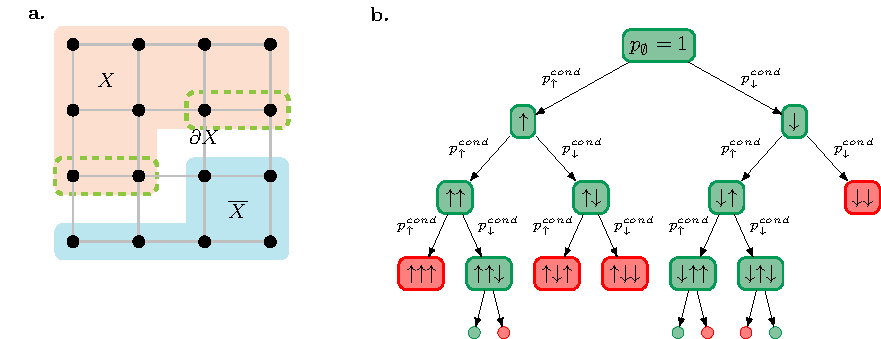
\includegraphics[width=\textwidth]{figures/squarelattice.pdf}
  \caption{\textbf{a.} An example Ising spin--glass  of 16 spins on a square lattice. The conditional probability for spins in the region $\overline{X}$ conditioned with a given configuration of spins in the region $X$ depends only on part of the configuration on the border $\partial X$. \textbf{b.} A fragment of state space tree. States kept at each level
    are marked with green, and the pruned branches are marked with red.}
  \label{fig:lattice-and-border}
\end{figure}

\begin{equation}
  \label{eq:conditional-prob}
  p(s_1, s_2, \ldots, s_k, s_{k+1}) = p(s_1, s_2, \ldots, s_k)p(s_{k+1}|, s_1, \ldots, s_k)
\end{equation}
We can exploit locality of the problem by observing that conditional
probability in \eqref{eq:conditional-prob} of configuration in the region $X =
  (1, 2, \ldots, k)$ depends only on configuration on the border $\partial X$ consisting of those spins, that directly interact with the region
$\overline{X} = (k+1, 2, \ldots N)$. To see that, denote by $H_X$ the usual
Hamiltonian $H$ restricted to the graph induced by vertices in $X$. Further,
let $H_{X, \overline{X}} = H - H_X - H_{\overline{X}}$. Notice that $H_{X,
    \overline{X}}$ contains only quadratic terms $J_{ij} s_i s_j$ such that $i \in
  X$ and $j \in \overline{X}$. Slightly abusing the notation, one may thus write
\begin{equation}
  H(s_1, \ldots, s_N) = H_X(s_1, \ldots, s_k) + H_{\overline{X}}(s_{k+1}, \ldots, s_N) + H_{X, \overline{X}}(s_1, \ldots, s_N)
\end{equation}
Using definition of conditional probability applied to Boltzmann distribution,
one thus gets
\begin{align}
  p(s_{k+1}|s_1, \ldots, s_k) & = \frac{\sum\limits_{(z_{k+2}, \ldots, z_N)}e^{-\beta H(s_1, \ldots, s_{k+1}, z_{k+2},\ldots,z_N)}}{\sum\limits_{(z_{k+1}, \ldots, z_N)}e^{-\beta H(s_1, \ldots, s_k, z_{k+1},\ldots,z_N)}}                                                                                                                                                     \\
                              & = \frac{\sum\limits_{(z_{k+2}, \ldots, z_N)}e^{-\beta (H_X(s_1, \ldots, s_k) + H_{\overline{X}}(s_{k+1}, z_{k+2},\ldots,z_N) + H_{X, \overline{X}}(s_1, \ldots, z_N))}}{\sum\limits_{(z_{k+1}, \ldots, z_N)}e^{-\beta (H_X(s_1, \ldots, s_k) + H_{\overline{X}}(z_{k+1}, \ldots,z_N) + H_{X, \overline{X}}(s_1, \ldots, z_N))}}                 \\
                              & = \frac{e^{-\beta H_X(s_1, \ldots, s_k)}\sum\limits_{(z_{k+2}, \ldots, z_N)} e^{-\beta(H_{\overline{X}}(s_{k+1}, z_{k+2},\ldots,z_N) + H_{X, \overline{X}}(s_1, \ldots, z_N))}}{e^{-\beta H_X(s_1, \ldots, s_k)}\sum\limits_{(z_{k+1}, \ldots, z_N)}e^{ -\beta(H_{\overline{X}}(z_{k+1}, \ldots,z_N) + H_{X, \overline{X}}(s_1, \ldots, z_N))}} \\
                              & = \frac{\sum\limits_{(z_{k+2}, \ldots, z_N)} e^{-\beta(H_{\overline{X}}(s_{k+1}, z_{k+2},\ldots,z_N) + H_{X, \overline{X}}(s_1, \ldots, z_N))}}{\sum\limits_{(z_{k+1}, \ldots, z_N)}e^{ -\beta(H_{\overline{X}}(z_{k+1}, \ldots,z_N) + H_{X, \overline{X}}(s_1, \ldots, z_N))}}
\end{align}
Note, in both numerator and denominator spins with indices from $X$ appear
non-trivially only in $H_{X, \overline{X}}$ , i.e. the whole expression depends
only on those spins in $X$ that directly interact with spins in $\overline{X}$,
which was to be demonstrated.

Before discussing how probabilities in \eqref{eq:conditional-prob} can be
computed, let us first extend the above approach to the more general case of a
quasi-two-dimensional graph, i.e. one in which nodes can be grouped into
\emph{clusters} forming a two-dimensional square lattice (see Fig.
\ref{fig:clustering} for details). One can easily see, that again we can
construct a tree-like structure representing state space, this time considering
joint configurations of spins in a single cluster. Therefore, for the most of
the time, we might "forget" the underlying spin-glass structure and consider
square lattices in which spin clusters act like higher-dimensional systems.

\begin{figure}
  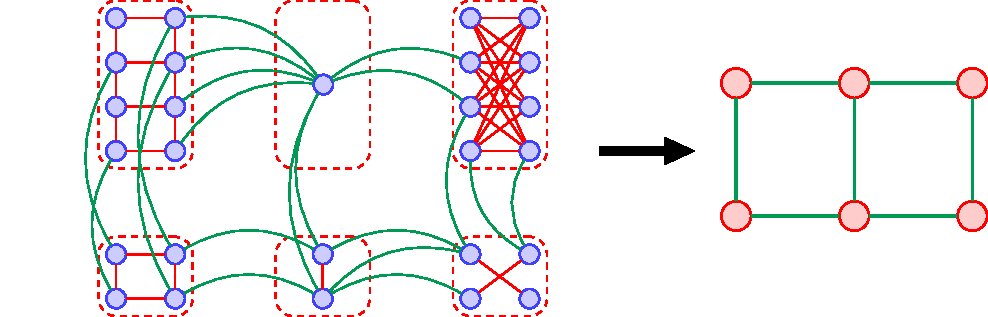
\includegraphics[width=\textwidth]{figures/clustering}
  \caption{Grouping spins into clusters in a Chimera-like graph.} \label{fig:clustering}
\end{figure}

A central object considered in our algorithm is the probability distribution
$\exp[-\beta H(\mathbf{s})]$, which we approximate using a PEPS-equivalent
tensor network, whose detail will be described shortly. Contracting such a
network can give the probability distribution of any full configuration, as
well as the marginal probabilities.

\begin{equation}
  p(s_1, s_2, \ldots, s_k) \sim \tr[\mathcal{P}_{(s_1, \ldots, s_k)} e^{-\beta H(\mathbf{s})}]
\end{equation}

\section{Grouping spins into clusters}
The outlined approach can be easily extended to the case of the problem defined
on a graph in which nodes can be grouped into \emph{clusters} forming a
two-dimensional lattice. See Fig. \ref{fig:quasi2d} for a detailed description.
In this more general case, $s_i$ in \eqref{eq:conditional-prob} denote join
probability of configuration in $i$-th cluster, and each configuration is
branched into $2^lM$ new ones, where $l$ is the number of spins in respective
cluster.

\section{PEPS network construction}
We begin construction of a PEPS network for a quasi-two-dimensional graph by
considering two spins at sites $i$ and $j$ connected by an edge $J_{ij}$. This
edge can be decomposed as

\begin{equation}
  e^{-\beta J_{ij}s_i s_j} = \sum_{\gamma = \pm 1} B^{s_{i\phantom{j}}}_\gamma C^{s_j}_\gamma
\end{equation}
where
\begin{equation}
  \label{eq:decomposition}
  B^{S_i}_\gamma = \delta_{\gamma s_i} \quad C^{s_j}_\gamma = e^{-\beta \gamma J_{ij} s_j}
\end{equation}
Note that decomposition \eqref{eq:decomposition}, although not unique, has the
advantage of comprising only non-negative coefficients, which positively
affects numerical stability. Next, with each cluster we associate a PEPS tensor
\begin{equation}
  \label{eq:peps}
  A^{\mathbf{s_c}}_{\mathbf{lrud}} = e^{-\beta H(\mathbf{s_c})} B^{\mathbf{s_c}^l}_\mathbf{l}C^{\mathbf{s_c}^r}_\mathbf{r}B^{\mathbf{s_c}^u}_\mathbf{u}C^{\mathbf{s_c}^d}_\mathbf{d}
\end{equation}
Here, $\mathbf{s_c}$ collects all spins in a given cluster, and
$\mathbf{s_c}^l$, $\mathbf{s_c}^r$, $\mathbf{s_c}^u$, $\mathbf{s_c}^d$ collect
spins interacting with it from the left, right, up and down respectively. Each
such tensor has five legs: the physical one $\mathbf{s_c}$ of dimension $2^m$,
where $m$ denotes the number of spins in the cluster, and the virtual ones $l,
  r, u, d$ with dimensions depending on the number of inter-cluster edges. Note
that $H$ in \eqref{eq:peps} is restricted to the graph induced by spins
belonging to the considered cluster. The construction is depicted in Fig.
\ref{fig:tensors}.

\begin{figure}
  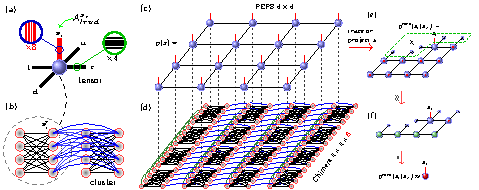
\includegraphics[width=\textwidth]{figures/peps.pdf}
  \caption{Construction of PEPS network} \label{fig:tensors}
\end{figure}

\section{Results}

To fully investigate the performance of our algorithm, we performed several
benchmarks, testing various metrics quantifying both execution time, as well as
the quality of the found solutions. We tested our algorithm for sets of
\emph{droplet} instances specifically designed to be hard for classical
heuristic solvers, especially ones relying on local updates. We benchmarked our
algorithm against classical solvers based on Parallel-Tempering and D-Wave
Quantum annealer DW-2000Q$_6$. As it is hard to directly compare samples
obtained from the D-Wave annealer with the output of our deterministic
algorithm, we decided to use time-to-solution as a metric. The time to solution
$\mbox{TTS}$ is defined as
\begin{equation}
  \label{eq;tts}
  \mbox{TTS} = \tau \frac{\log(1 - p_{target})}{\log(1 - p_{succ})},
\end{equation}
where $p_{target}$ is the desired probability of obtaining solution, $p_{succ}$
is the empirical probability of obtaining solution and $\tau$ is the running
time of the solver. In addition, for D-Wave annealers we multiply $\mbox{TTS}$
by the ratio $N/\mbox{num\_qubits}$, to account for the possibility of fitting
multiple instances of the problem on the device at the same time. Naturally,
one might consider $\mbox{TTS}$ metric not only for finding a ground state, but
also for finding a solution approximating a ground state with a given
approximation ratio ground state (i.e. solution lying in the desired lowest
fraction of the full energy spectrum). The results of these benchmarks are
presented in Table \ref{tab:tnvspt}. For all instances, our algorithm was able
to find the ground state, which was not the case for other solvers. However, if
one is not necessarily interested in finding the ground state, both D-Wave
annealers and classical Parallel Tempering solver might find a satisfying
solution in a shorter time.
\begin{table}[b]
  \centering
  \begin{tabular}{|l|c|ccc|}
    \hline
    \rowcolor{theader}  Method & approx. ratio & $N=512$   & $N=1152$  & $N=2048$  \\
    \hline
    TN                         & g.s.          & 30s       & 150s      & 450s      \\
    \hline
    \hline
    PT (adaptive)              & g.s.          & 800s      & ---       & ---       \\
    \hline
    PT (geometric)             & $0.01$        & 0.53s     & 4.16s     & ---       \\
    PT (geometric)             & $0.005$       & 2.51s     & 56.4s     & ---       \\
    PT (geometric)             & $0.001$       & 158.4s    & timed-out & ---       \\
    PT (geometric)             & $0.0001$      & 897.6s    & timed-out & ---       \\
    \hline
    \hline
    DWave 2000Q$_6$            & $0.01$        & $0.003$s  & $0.006$s  & $0.02$s   \\
    DWave 2000Q$_6$            & $0.005$       & $0.2$s    & timed-out & timed-out \\
    DWave 2000Q$_6$            & $0.001$       & timed-out & timed-out & timed-out \\
    \hline
    \hline
  \end{tabular}
  \caption{Comparison of time-to-solution metric for our tensor network based algorithm,
    in-house parallel tempering implementation and D-Wave 2000Q$_{6}$. The
    \emph{adaptive} and \emph{geometric} terms refer to the distribution of inverse
    temperature in Parallel Tempering replicas.} \label{tab:tnvspt}
\end{table}
%%% Local Variables:
%%% mode: latex
%%% TeX-master: "../main"
%%% End:

%\chaptermark{}ter{Finding low--energy spectrum of spin glass using CUDA}
\chapter[Brute--forcing spin--glass problems]{Brute--forcing spin--glass problems with CUDA}
\label{chapter:bruteforce}
In chapter \ref{chapter:tn} we presented a tensor network--based heuristic algorithm
tailored for Ising spin--glass problems defined on Chimera graphs. In stark contrast, in this
chapter we will shift our attention to a deterministic algorithm capable of solving problems defined
on arbitrary (but relatively small) graphs.

Conceptually, the simplest approach for solving any optimization problem is a
brute force approach, i.e. an exhaustive search through the set of all possible
solutions. For the QUBO or Ising spin--glass with $N$ variables, this would
require iterating over $2^{N}$ possible states and computing energy for each of
them, resulting in a superexponential algorithm. Although the approach is
clearly infeasible for large problems, it presents several advantages. The
algorithm is deterministic and can certify\footnote{i.e., prove that the found
  solution is in fact optimal} the solution. Moreover, it can be used to compute
a low energy spectrum of arbitrary size $k$ (provided that it can fit into
memory). Lastly, it is trivially parallelizable and hence can be efficiently
accelerated using virtually any parallel computing paradigm, thus significantly
increasing attainable problem sizes.

In this chapter, we discuss such a brute--force algorithm using massively
parallel CUDA architecture. We start by outlining the basic version of the
algorithm and then discuss its recent optimizations for cases when the goal is
to find only the ground state (as opposed to finding a low energy spectrum).
Our implementation is capable of finding the ground state of instances of size
$N=54$ in an hour using a commodity GPU and achieving the same task in less
than 5 minutes on a server-grade NVIDIA DGX H100. Lastly, we present a possible
application of our algorithm, which is validating a recent MPS--based algorithm
for solving Ising spin--glasses.

% Optimization problems play an important role in modern society, especially in current volatile times. Instances of such problems can be found in numerous areas of industry and applied sciences. One could mention logistic issues, such as vehicle routing problem together with its variants, and the famous protein folding problem or job shop scheduling to name just a few. It is often the case where many of the aforementioned problems fall into the so called NP--hard complexity class. This fact alone renders hard to solve, making the entire operational research a challenging endeavour requiring enormous amount of computational resources.

% One way to tackle optimization problems is an exhaustive search over all possible solutions. Unfortunately, such brute--force approach quickly becomes impractical, as the number of possible solutions increases exponentially with the problem size. Nevertheless, despite its simplicity and obvious limitations, the brute--force algorithm is often the only approach capable of solving and certifying~\footnote{(i.e., proving that the found solution is in fact optimal)} \textit{arbitrary} problem instances within a given complexity class. For this very reason, efficient brute--force solvers are still considered to be an irreplaceable tool for testing and benchmarking other, often way more sophisticated, algorithms.

\section{Finding low--energy spectrum with CUDA}
\subsection{Outline of the algorithm}
An idealized brute force algorithm for solving QUBO problems running on a
hardware with infinite storage and an infinite number of execution units can be
summarized as follows:
\begin{enumerate}
  \item Launch number of threads equal to the total number of possible states.
  \item Let each thread compute the energy of one of the states.
  \item Extract (e.g. by sorting) the desired number of low--energy states.
\end{enumerate}
Naturally, an attempt to implement such an algorithm on real hardware is doomed
to fail. To exemplify this, consider a problem with $N=40$ variables. Assuming
we use 32-bit floating point numbers, one would need an enormous amount of
$2^{40}\cdot 4B = 4398046511104\mbox{B}$, or $4\mbox{TB}$ of working memory to
store the computed energies. For $N=50$, this number grows to $4096\mbox{TB}$.
Clearly, such an amount of needed memory is prohibitively large, and that is
even before we consider some form of storage for system states. Moreover, no
current hardware can execute $2^{40}$ threads in parallel. Fortunately, we can
adapt our algorithm to take into account limited memory and parallelism. To do
so, we introduce the following assumptions:
\begin{enumerate}
  \item We will process the solution space in \emph{chunks} that can fit into GPU
    memory.
  \item Number of states in a chunk can be larger than the total number of threads.
    Should this be the case, the threads will process the chunk using a
    grid--stride loop pattern.
\end{enumerate}
As an added benefit of our assumptions, we decouple the grid size from the
problem size. The number of thread blocks and block size become parameters of
our algorithm, which facilitates further fine-tuning of the kernel execution
parameters.

The algorithm will keep track of $k$ lowest--energy states computed so far.
This information will be updated after each new chunk is processed. The
downside of this approach is that the size of the low-energy spectrum we can
compute is limited by the chunk size. However, this limitation is not as severe
as it seems, because in a typical scenario, we have $k \ll 2^{N}$.

In the next section, we discuss another important aspect of our algorithm,
which is efficient storage and representation of system states.

\subsection{Storage and representation of system states}
Implementing efficient algorithms involves choosing the right storage strategy
for the data the algorithm operates on. This is especially the case for
present-day GPUs, which are equipped with fairly limited memory, as compared to
the operating memory available to the traditional CPU. Moreover, memory
transfers between host and GPU induce additional overhead that should be
avoided whenever possible. For this reasons one often aims for designing the
storage strategy such that it reuses information already available on the GPU
as much as possible, thus optimizing resource usage and minimizing the number
of memory transfers.

In principle, each configuration of a $N$--variable QUBO can be represented by
$N$ integers. However, since each variable can be assigned only one of two
possible values, this wastes a lot of available memory, as out of each machine
word only a single bit is used. Instead, one can pack the whole state of the
system into a single integer by identifying each bit of the underlying machine
word with a single spin. In our implementation, we decided to use 64-bit
integers. This particular implementation choice limits attainable problem sizes
to $N=64$. However, considering that solving larger problems using the brute
force approach is not likely to be possible in the near future (as demonstrated
by our benchmarks presented further in this chapter), this is not a significant
limitation. Furthermore, should the need arise, one could extend the
implementation to use multiple 64-bit integers for storing a single
configuration.

Identifying states with integers greatly simplifies their enumeration, as it
boils down to iterating over an appropriate range of natural numbers. More
importantly, it allows GPU threads to identify the system state they have to
process using their index and additional offset designating the chunk. In our
implementation, we restrict ourselves to chunk sizes being power of two, i.e.
chunk size $=2^{M}$ for some $M < N$. We conceptually split each configuration
into two parts:
\begin{enumerate}
  \item A \emph{local} part comprising least significant $M$ bits. This is part is
    \emph{different} for each state in the chunk.
  \item A \emph{suffix} comprising the most significant $N-M$ bits. This part is
    \emph{the same} for each state in the chunk.
\end{enumerate}
Now, since there are $2^{N-M}$ chunks, we can identify each chunk with a $N-M$
bit number. Finally we arrive for a formula for an integer representation
$\mathbf{q}_{i}^{j}$ of an $i$-th configuration in $j$-th chunk:
\begin{equation}
  \mathbf{q}_{i}^{j} = i + 2^{M}\cdot j,\qquad i=0,\ldots,2^{M}-1, \; j=0,\ldots,2^{N-M}-1
\end{equation}
The following example demonstrates the representation described above in
detail.
\begin{example}[Processing solution space in chunks]
  Consider QUBO with $N=8$ variables. We decide to use $M=5$. Hence, there are
  $2^{M}=32$ states in each chunk and a total of $2^{N-M}=8$ chunks. The
  \emph{local} part of the first state in each chunk is $0$, or $(00000000)_{2}$
  in binary. The local part of the last state in each chunk is $31$, or
  $(00011111)_{2}$. The table \ref{tab:chunks} below enumerates ranges of
  combined integer representation of states in each chunk.
  \begin{table}[ht!]
    \centering
    \begin{tabular}{|c|c|c|c|c|c|}
      \hline
      \rowcolor{theader}
      \multicolumn{2}{|c|}{Chunk}      &
      \multicolumn{2}{c|}{First state} &
      \multicolumn{2}{c|}{Last state}                                                                        \\
      \hline
      \rowcolor{tsubheader} Index      & Binary    & Decimal & Binary           & Decimal & Binary           \\
      \hline
      0                                & $(000)_2$ & 0       & $(00000000)_{2}$ & 31      & $(00011111)_{2}$ \\
      1                                & $(001)_2$ & 32      & $(00100000)_{2}$ & 63      & $(00111111)_{2}$ \\
      2                                & $(010)_2$ & 64      & $(01000000)_{2}$ & 95      & $(01011111)_{2}$ \\
      3                                & $(011)_2$ & 96      & $(01100000)_{2}$ & 127     & $(01111111)_{2}$ \\
      4                                & $(100)_2$ & 128     & $(10000000)_{2}$ & 159     & $(10011111)_{2}$ \\
      5                                & $(101)_2$ & 160     & $(10100000)_{2}$ & 191     & $(10111111)_{2}$ \\
      6                                & $(110)_2$ & 192     & $(11000000)_{2}$ & 223     & $(11011111)_{2}$ \\
      7                                & $(111)_2$ & 224     & $(11100000)_{2}$ & 255     & $(11111111)_{2}$ \\
      \hline
    \end{tabular}
    \caption{An example enumeration of chunks iterated over by brute force algorithm.}
    \label{tab:chunks}
  \end{table}

  \begin{table}{}

  \end{table}
\end{example}

\subsection{Implementation details}

In our approach we decided to store states and their corresponding energies in
arrays of size $k+2^{M}$, where $k$ is the desired size of the low energy
spectrum and $2^{M}$ is the chunk size. The arrays are always synchronized,
i.e. at all times $i$-th state corresponds to $i$-th energy. The first $k$
elements store the lowest energies and corresponding configurations found so
far. When a new chunk is being processed, the second part of the arrays is
populated with new states and energies by the energy--computing kernel. Next,
the best $k$ states from the current chunk are selected and moved into indices
$k, k+1,\ldots,2k-1$. In this way, the global best solutions from previous
chunks and the lowest energy states from the current chunk in a continuous
space in memory, which facilitates updating the best configurations.

One could use a parallel sorting procedure for extracting the $k$
lowest--energy states at each step. However, for improved performance, we
decided to use a combination of the \texttt{bucketSelect} \cite{bucketselect}
algorithm in tandem with \texttt{thrust::partition\_by\_key} \cite{thrust}. The
\texttt{bucketSelect} algorithm is used to find the pivot configuration that
would reside at $k$--th position in the sorted array. Then,
\texttt{thrust::partition\_by\_key} is used to reorder both arrays such that
the configurations with energies lower than the one of the pivot are moved to
the beginning. The same procedure is used both for extracting the $k$-lowest
energy states in the given chunk, as well as to update the global solution by
extracting $k$-lowest energy configurations from the first $2k$ configurations.
The whole procedure is depicted in Fig. \ref{fig:bruteforce}.

Lastly, we would like to note that the algorithm we just described can also be
implemented on homogenous, CPU-only architectures using any of the available
parallelization approaches. In our implementation, we used the
OpenMP\cite{openmp} for a CPU--only version.

\begin{figure}
  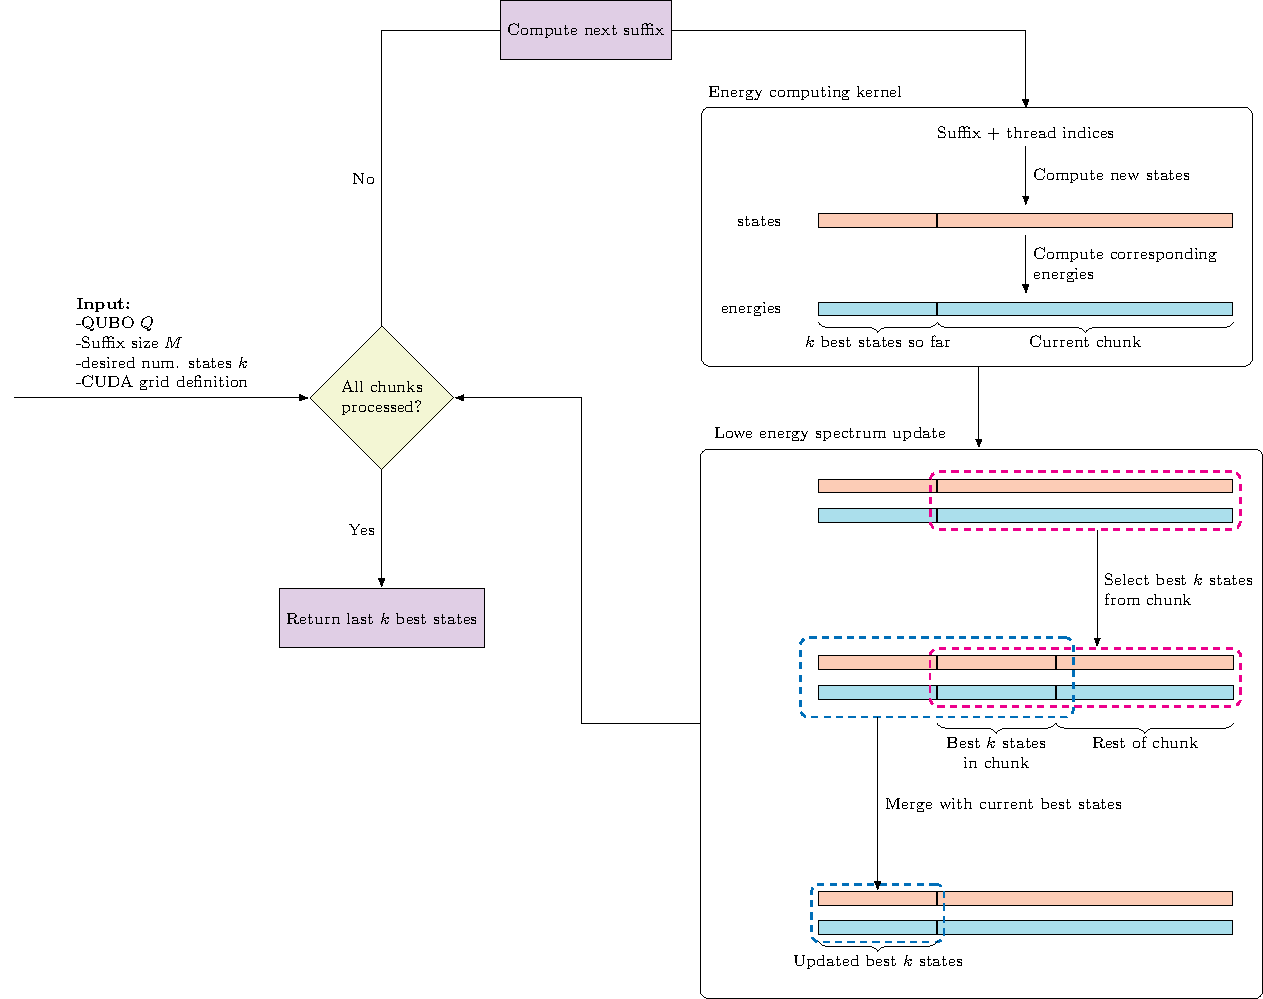
\includegraphics[width=\textwidth]{figures/bruteforce}
  \caption{
    Detailed representation of brute force algorithm for finding $k$-lowest energy
    states of a QUBO. The algorithm iterates over the set of all possible states in
    chunks of size $2^{M}$, where $M$ is a user-defined parameter. Throughout the
    algorithm execution, we maintain arrays of states and corresponding energies.
    The first part of those arrays stores the $k$ best configurations encountered
    so far, and the second part stores configurations belonging to the currently
    processed chunk. In the first phase of the iteration, an energy-computing
    kernel is launched. Then, the $k$--lowest energy configurations from the given
    chunk are selected and moved towards the part of the array with the current
    best solutions. Finally, the best $k$ states are selected from the first $2k$
    configurations and the algorithm proceeds to the next chunk or terminates if
    all the chunks have been iterated over. } \label{fig:bruteforce}
\end{figure}

\subsection{Performance benchmarks}
In order to test the performance of our algorithm, we run extensive benchmarks
using the following hardware:
%
\begin{itemize}
  \item CPU:
    \href{https://ark.intel.com/products/94456/Intel-Core-i7-6950X-Processor-Extreme-Edition-25M-Cache-up-to-3-50-GHz-}{$10$
      Cores {\rmfamily Intel\textregistered} Core \textsuperscript{TM}i7-6950X};
    %
  \item GPU(1):
    \href{https://www.nvidia.com/en-us/geforce/products/10series/geforce-gtx-1080}{Nvidia
      GeForce GTX $1080$, $8$GB GDDR$5$ global memory, $2560$ CUDA Cores};
    %
  \item  GPU(2): \href{https://www.nvidia.com/en-us/titan/titan-v/}{Nvidia Titan V,
      $12$GB HBM$2$ global memory, $5120$ CUDA Cores}.
\end{itemize}

For conducting our benchmarks we generated $100$ spin-glass instances for each
$N=24, 26, \ldots, 30, 32$. Additionally, we generated $100$ instances of size
$N=40$ and single instances of sizes $N=48, 50$ that were feasible to solve
with Titan V GPU (which was the most powerful card available to us at the time
of performing the benchmarks). Coefficients of each spin-glass were drawn
randomly from uniform distributions on the intervals $[-2, 2]$ and $[-1, 1]$
for magnetic fields and couplings respectively. For each instance, we computed
the low energy spectrum of $k=100$ states with our algorithm. We used a maximum
chunk size of $2^{29}$ for Titan V and CPU and the chunk size of $2^{27}$ for
GTX 1080. As already mentioned, larger instances $(N > 32)$ were solved only
using Titan V GPU. For GTX 1080 and CPU implementation, the expected time to
solve those instances was estimated based on the timings for smaller $N$. The
results of our benchmarks are presented in Fig. \ref{fig:benchmark_results}.

\begin{figure}
  \centering
  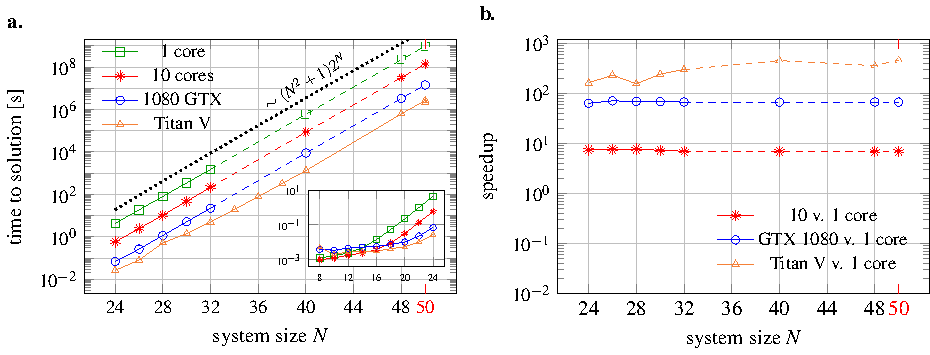
\includegraphics[width=\textwidth]{figures/resultsplot_reduced.pdf}
  \caption{Results of benchmarks of our algorithm. {\textbf{a.}} Time to solution vs.
    system size $N$. {\textbf{b.}} Speedup of multi-core/GPU implementation with
    respect to a single core one vs. system size $N$. The solid lines represent the
    numerical results and the dashed lines present estimates based on results
    obtained for smaller system sizes.} \label{fig:benchmark_results}
\end{figure}

\section[Example application]{Example application: verifying MPS-based optimization algorithm}

As an example application, in this section, we use our brute-force-based
approach with heuristic algorithm based on Matrix Product States (MPS). The
detailed description of this algorithm is outside the scope of this thesis, and
we refer the interested reader to the Supplementary Material in \cite{tn}.
Nevertheless, before we outline how the algorithm works.

Similarly to the algorithm presented in chapter \ref{chapter:tn}, in the
MPS--based approach one explores the probability distribution (as opposed to
exploring the energy landscape directly). The basic idea behind is to
approximate Boltzmann distribution as
\begin{equation}
  e^{-\beta H(\mathbf{s})/2} \approx A^{s_1} A^{s_2} \ldots A^{s_L} = |\Psi(\beta) \rangle,
  \label{eq:mps}
\end{equation}
for large enough $\beta$. Here, $A^{s_{i}}$ are real matrices of limited
dimension $\le D$. In this context, the parameter $D$ is referred to as the
\emph{bond dimension}. Fig. \ref{fig:mps:boltzmann} shows a pictorial
representation of such approximation. At each bond, the system is split into
two halves. An exact decomposition would require bond $D$ of exponential
(w.r.t. number of spins) size. Limiting $D$ effectively limits the amount of
entanglement related to given bipartition \cite{Wall18}. Once the approximation
in the equation \eqref{eq:mps} is constructed, it is possible to effectively
compute any marginal or conditional probability, and then systematically search
for the most probable (and thus, ones with lowest energy) classical
configurations using branch-and-bound procedure, constructing tree of most
probable spin configurations one variable at the time.

The search starts with $\beta=0$, for which the MPS decomposition is trivial.
Then, the algorithm subsequently simulates the imaginary time evolution by
applying the sequence of gates:
\begin{equation}
  \label{eq:gate}
  U_i(d\beta) = e^{-d\beta s_i (\sum_{j>i}J_{ij}  s_j+h_i)/2},
\end{equation}
which totals to $\prod_{i=1}^N U_i(d\beta) = e^{-d \beta H(\mathbf{s})/2}$. One
can observe that applying each gate results in the doubling of the bond
dimension. Hence, at each step, one has to systematically find an approximation
maintaining the fixed $D$. The whole procedure is depicted in Fig.
\ref{fig:mps:compress}.

\begin{figure}
  \begin{subfigure}[t]{0.45\textwidth}
    \caption{}\label{fig:mps:boltzmann}
    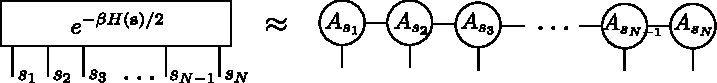
\includegraphics[width=\textwidth]{figures/mps}
  \end{subfigure}\hfill
  \begin{subfigure}[t]{0.45\textwidth}
    \caption{}\label{fig:mps:compress}
    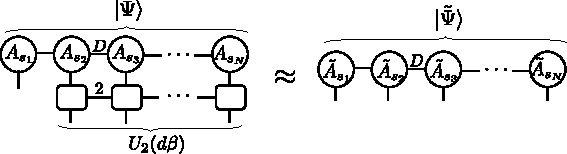
\includegraphics[width=\textwidth]{figures/mps_compress}
  \end{subfigure}
  \caption{\subref{fig:mps:boltzmann} Approximation of the Boltzmann distribution using the MPS ansatz. \subref{fig:mps:compress} Compression scheme used in the MPS algorithm.}
  \label{fig:mps}
\end{figure}

By construction, the MPS-based ansatz outlined above is one-dimensional. Hence,
the question is to what end can it be used to find low-energy solutions of
spin-glasses defined on a complete graph? To answer this question, we ran the
MPS-based algorithm on 100 instances of different sizes and then compared the
results to the output of our brute-force algorithm. Instances were drawn at
random using the same procedure as described in the previous section. The
results of these tests are depicted in Fig. \ref{fig:mpsbench}. One can observe
that bond dimension $D=128$ and inverse temperature $\beta=1$ are already
sufficient to find the ground state of all the test instances, and recover most
of the $k=1000$ lowest energy states. The results also demonstrate the
significance of setting the time-step parameter $d\beta$ to small enough value.
As the last conclusion from our benchmarks, we would like to point out the
magnitude of compression of the relevant information in the MPS representation.
Indeed, an exact MPS decomposition would require the bond dimension $D=2^{N/2}
\gg 128$.

\begin{figure}[th]
  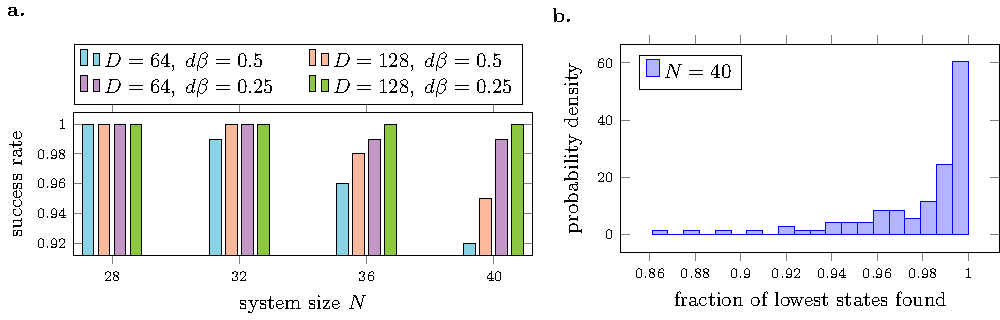
\includegraphics[width=\textwidth]{figures/mps_benchmark}
  \caption{Results of the MPS benchmarks. In both panels $\beta=1$. \textbf{a.} Success
    rate, defined as a fraction of instances (out of 100) for which the MPS
    algorithm found the ground state. \textbf{b.} Normalized histogram showing the
    number of instances for which the MPS algorithm was able to find the given
    fraction of lowest $k=1000$ states.} \label{fig:mpsbench}
\end{figure}

\section{Improving the algorithm using Gray Code}

The algorithm presented in the previous chapter is already highly performant. However, we can still improve
upon it by altering the order in which we enumerate the integral representation
of states used by our algorithm.

\subsection{Single bit--energy difference}
Suppose we are given a QUBO with $F(q_{1},\ldots,q_{N})$ as in the equation
\eqref{eq:qubo}. Consider two states, say $\bq{1} = (\q{1}_{1},\ldots,\q{1}_{N})$
and $\bq{2}=(\q{2}_{1},\ldots,\q{2}_{N})$ such that they only differ in the
$k$-th bit, i.e. $\q{2}_{k}=1-\q{1}_{k}$ and $\q{2}_{i}=\q{1}_{i}$ for $i \ne
  k$. The energy difference $F(\bq{2})-F(\bq{1})$ can be easily computed and the
formula reads
\begin{align}
  \begin{split}
    \label{eq:energydiff1}
    F(\bq{2})-F(\bq{1}) &= b_{k}(\q{2}_{k}-\q{1}_{k}) + \sum_{i\ne k}a_{ik}\q{1}_{i}(\q{2}_{k} - \q{1}_{k}) \\
    &= (\q{2}_{k}-\q{1}_{k}) \left(b_{1} + \sum_{i \ne k}a_{ik}\q{1}_{i}\right) \\
    & = (1-2\q{1}_{k}) \left(b_{k} + \sum_{i \ne k}a_{ik}\q{1}_{i}\right).
  \end{split}
\end{align}
Interestingly, computing the difference in equation \eqref{eq:energydiff1}
requires only $O(N)$ multiplications. But how can this be used to improve the
performance of the exhaustive search through QUBO state space?

Moving $F(\bq{1})$ to the right-hand side, we obtain a formula for $F(\bq{2})$,
which allows for computing it with only $N+1$ instead of maximum of $N(N+1)/2$
multiplications, provided that $F(\bq{1})$ is known. Remember that this is only
possible because $\bq{1}$ and $\bq{2}$ differ only by a single bit. If we could
enumerate states in such a fashion that every consecutive two states differ
only by a single bit, we could leverage the above formula instead of
recomputing energy for each state from scratch. Before we describe how the
procedure works and how to implement this on GPU, let us first introduce the
necessary notation. Given a state $\mathbf{q} = (q_{1},\ldots,q_{N})$, by
$\flip{\mathbf{q}}{k}$ we will denote a state resulting from flipping $k$-th
bit of $\mathbf{q}$, i.e.
\begin{equation}
  \flip{\mathbf{q}}{k} \coloneq (q_{1}, \ldots, q_{k-1}, 1-q_{k}, q_{k+1}, \ldots, q_{N})
\end{equation}
and by $\diff_{F}(\mathbf{q},k)$ we will denote the difference between the
energies of $\flip{\mathbf{q}}{k}$ and $\mathbf{q}$. Using the equation
\eqref{eq:energydiff1}, we see that the expression for
$\diff_{F}(\mathbf{q},k)$ is
\begin{align}
  \begin{split}
    \diff_{F}(\mathbf{q},k) = F(\flip{\mathbf{q}}{k}) - F(\mathbf{q}).
  \end{split}
\end{align}
The pseudocode for a serial algorithm for solving a QUBO problem using our
observations is outlined in listing \ref{lst:grayserial}. Before we can
implement it on GPU though, we need to answer the following questions:
\begin{listing}
\begin{minted}{python}
def solve_qubo(F, q):
    q = [0] * N # Start with all bits set to 0
    best_state = current_state = q
    best_energy = current_energy = F(q)

    for i in range(2 ** N - 1):
        k = find_next_bit_to_flip(i)
        current_energy = current_energy + diff(q, k)
        current_state = flip(q, k)
        if current_energy < best_energy:
            best_energy = current_energy
            best_state = current_state
    return best_state, best_energy
\end{minted}
\caption{Pseudocode for algorithm solving the QUBO problem using energy differences and bit flips.}
\label{lst:grayserial}
\end{listing}
\begin{enumerate}
  \item How to produce a sequence of $2^{N}-1$ bits such that executing them enumerates
    a rll possible states?
  \item How to divide work among CUDA threads?
\end{enumerate}
The answer to the first question is well-known and involves enumerating
integers using the Gray code, which we will describe now.

\subsection{Gray code}
When one talks about a binary encoding of integers, the first thing that comes
to mind is a usual positional base-2 system. This encoding certainly does not
fit our purpose. Indeed, suppose $N=3$ and we are currently processing state
corresponding to number $3$, whose representation in binary is $(011)_{2}$. The
next state, corresponding to $4$ is encoded by the string $(100)_{2}$, which
differs in all three bits.

Instead of using the positional system, we might utilize an encoding called
Gray code, or Reflected Binary Code (RBC) \cite{gray,lucal1959}, which is primarily used to improve
the robustness of electromechanical switches and in the error correction protocols.
In this code, encoding of two successive integers always differs by at most one
bit, which makes it suitable for application in our algorithm.

The conceptual construction of the Gray code is straightforward. For Gray code of
length $1$ we have two binary strings: $0$ and $1$. To obtain all Gray codes
for a given length $N > 1$, we first construct an ordered list of codes of
length $N-1$ and call it $L$. Then, we reverse the list of codes and call it
$H$, an operation called \emph{reflection}. Finally, we prepend $0$ to all
elements of $L$ and prepend $1$ to all elements of $H$. The concatenation of
$L$ and $H$ forms the $N$--bit Gray Code. The process is illustrated in Fig.
\ref{fig:gray}. One useful consequence of the construction is that the shorter
Gray code might be viewed as an initial part of the larger one prepended with
enough zeros. Thus, statements like ``$n$-th Gray code'' make sense and are
unambiguous.

\begin{figure}
  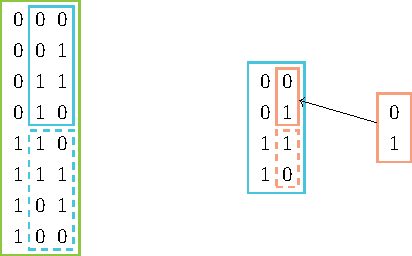
\includegraphics[width=\textwidth]{figures/gray.pdf}
  \caption{Reflection--based construction of Gray code. The length of the code is denoted
    by $N$. For $N=1$, the code comprises two binary strings, $0$ and $1$. To
    construct the code of length $N>1$, the code of length $N-1$ and its vertical
    reflection are stacked. Then, the first, unreflected half is prepended with $0$
    while the second, reflected half is prepended with $1$.} \label{fig:gray}
\end{figure}

An important thing to observe is that in our algorithm we need at most two Gray
code-encoded numbers at the time to determine the bit to be flipped. The
reflection--based construction outlined so far would require precomputing a
large part (if not all) of the encodings at once. Considering the size of the
state space, this is clearly infeasible. However, there exists an explicit
formula for computing $n$-th Gray code, which reads \cite{grayalgo}:
\begin{equation}
  \mbox{gray}(n) = n \oplus (n >> 1),
\end{equation}
where $\oplus$ denotes the bitwise xor operation and $>>$ is right bitshift.

To compute which bit differs between consecutive Gray codes, we can xor them,
and then find the position of the only set bit in the resulting integer. One
can easily implement a function that finds the first set bit in a 64-bit
integer, or use one of the available library or compiler built-in functions. For
instance, POSIX--compatible C standard libraries include \texttt{ffsll}
function \cite{ffs}. In CUDA, there is a \texttt{\_\_ffsll} function available \cite{CUDAguide}. For both
of the above cases, the function counts bits from $1$. Using this convention,
we can write a pseudocode for a function \texttt{find\_bit\_to\_flip} from
listing \ref{lst:grayserial} like in the listing~\ref{lst:findbit}.

\begin{listing}
\begin{minted}{python}
def find_bit_to_flip(i): # i starts from 0
    return ffs(gray(i) ^ gray(i+1))
\end{minted}
\caption{Pseudocode for a function generating bit flips for Gray code construction}
\label{lst:findbit}
\end{listing}

Now that we know how to construct a correct sequence of bit flips, it is time
we design a parallelization strategy, which is what we will do next.

\subsection{Parallelization using GPU}
The algorithm presented in \ref{lst:grayserial} is fully serial. Our task is
now to parallelize it so that it can be executed on GPU. Unsurprisingly, we
will once again employ the strategy of dividing each state into a suffix and a
prefix part. This time, however, it is the suffix that will stay fixed between
iterations. The prefix part will be updated in each iteration by flipping a
single bit in Gray code order. The process is illustrated in Fig.
\ref{fig:grayparallel}.

\begin{figure}
  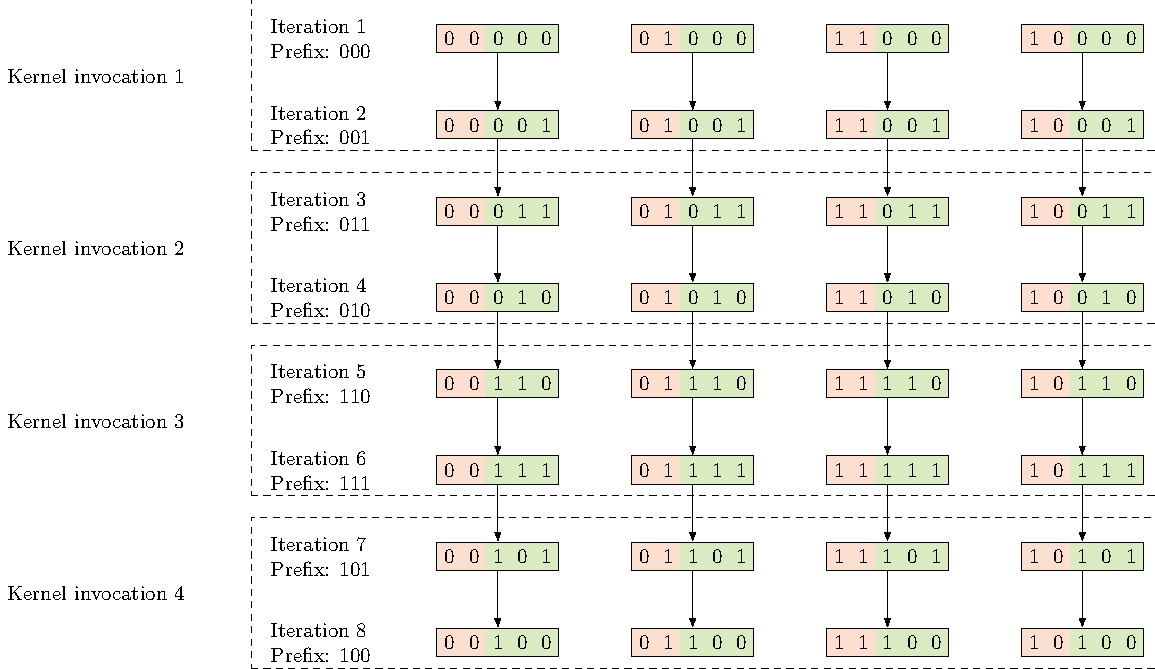
\includegraphics[width=\textwidth]{figures/grayparallel}
  \caption{
    Parallel processing of $N=5$--variable QUBO configurations in Gray code order. In
    our example, suffix length $M=2$, and hence $2^{M}=4$ states are processed in
    each iteration. Consequently, there are $2^{N-M}=8$ iterations. For this
    example, we consider a kernel that processes two iterations per kernel
    invocation, resulting in $2^{N-M}/2 = 4$ kernel invocations total. }
  \label{fig:grayparallel}
\end{figure}

Throughout the execution of the algorithm, we maintain four arrays of size
$2^{M}$. In each array, the $i$-th item always corresponds to the $i$-th
suffix. The \texttt{best\_states} and \texttt{best\_energies} arrays store the
best states found so far amongst states with $i$-th suffix. The
\texttt{current\_states} and \texttt{current\_energies} store configuration and
corresponding energy of current state being processed for $i$-th suffix. Each
iteration starts by determining the index of the next bit to be flipped. This
value is the same for all suffixes. Next, the algorithm computes energy
difference using the equation \ref{eq:energydiff1} and updates the
corresponding energy accordingly. After all $2^{N-M}$ iterations, the
\texttt{best\_states} and \texttt{best\_energies} arrays are used to extract
the ground state.

It is crucial to note that since we are only interested in finding the ground
state, we can group several iterations in one kernel invocation. In fact, it is
entirely possible to implement a kernel that runs all the iterations, which
would avoid kernel launch overhead. Moreover, such kernel could use
thread--local variables to store current state and energy instead of using
global arrays, which would further increase performance. However, as we will
see further in this chapter, we will propose further optimizations that would
require us to split the algorithm into several kernel invocations.

\subsection{Further optimizing parallel execution}

There are two optimizations we can make to further reduce the number of
operations performed in each iteration. Let us first notice that the only bit
flips that can happen, do so in the prefix part. Going back to the equation
\eqref{eq:energydiff1}, we can rewrite the expression for $F(\bq{2})-F(\bq{1})$
into a sum of two parts:
\begin{align}
  F(\bq{2})-F(\bq{1}) = & (1-2\q{1}_{k}) \left(b_{k} + \sum_{i=0,i\ne k}^{N-M-1}a_{ik}\q{1}_{i}\right) + \label{eq:energydiff2} \\
                        & (1-2\q{1}_{k}) \left(b_{k} + \sum_{i=N-M}^{N-1}a_{ik}\q{1}_{i}\right)\label{eq:energydiff3}
\end{align}
Since the first summand \eqref{eq:energydiff2} is independent from the suffix,
which means that for each of the considered suffixes in any given iteration, it
has the same value. Since the states in the iteration are processed in parallel
by GPU threads, we have to either redo the same computation multiple times, or
use some synchronization mechanism, e.g. compute the prefix in one thread in
each block and then propagate the result to the whole block through shared
memory. However, there is a third approach. For each iteration, we compute the
prefix part of the energy difference using CPU, and then use it as a kernel
parameter. More precisely, we compute $L$ values of the prefix part of the
energy difference and pass it to the kernel as an additional array. Since the
information about which bit to flip is also relevant, we pass the bit sequence
as another array as well.

As for the \eqref{eq:energydiff3} part, observe that for each given prefix
there are only $N-M$ possible values of $k$ (again, that's because the bit
flips happen only in the prefix part, and there are $N-M$ prefix bits).
However, not all values of $k$ are equally common. Examining the Gray code
construction (c.f. Fig. \ref{fig:gray}) reveals that the least significant bit
flips half of times and the second least significant bit flips a quarter of
times. Generally, for $k=0,\ldots,N-M-1$ the $k$-th bit flips constitutes
approximately \footnote{Approximately, because there is an odd number of
  $2^{N-M}$ -1 flips performed, because we do not perform last bit flip which
  would take us back to $(0,\ldots,0)_2$ prefix.} $1/2^{k+1}$ of times.
Therefore, we can cache the value of \eqref{eq:energydiff3} for the $K$ most
commonly--occuring bit flips, where $K$ is a user--controlled parameter.

\begin{figure}
  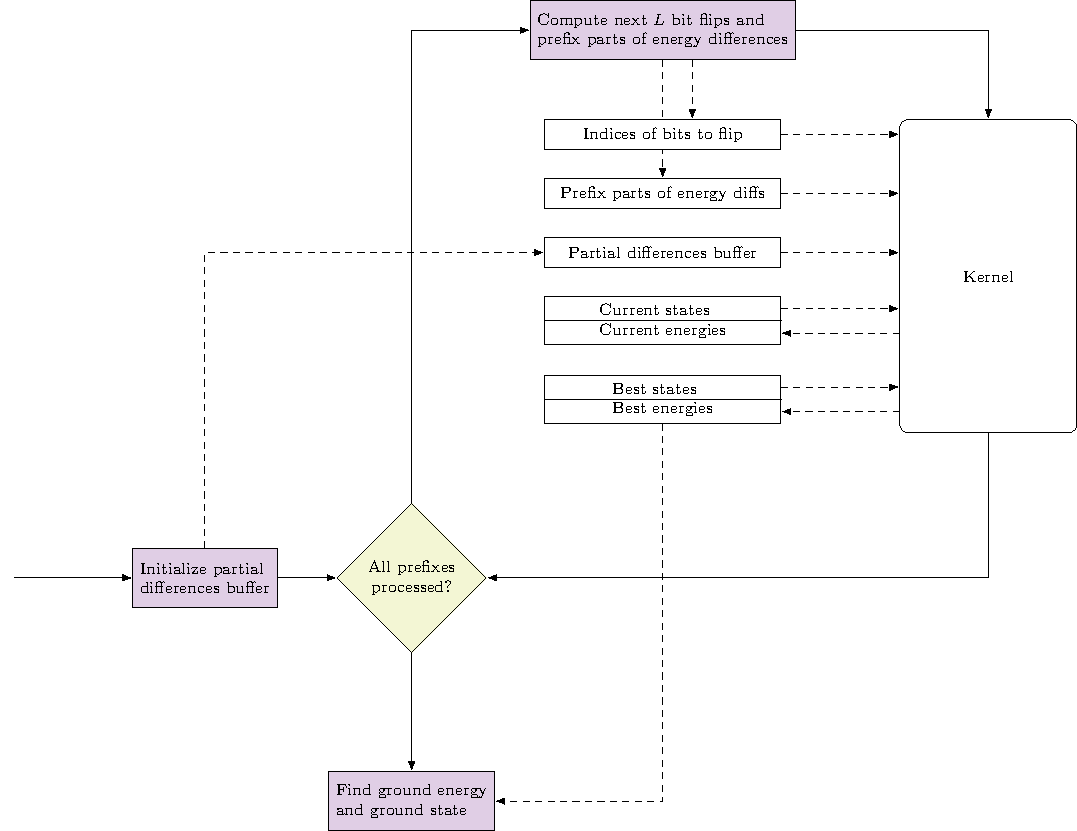
\includegraphics[width=\textwidth]{figures/bruteforcegray}
  \caption{
    Schematic representation of the GPU--enabled brute force algorithm for finding
    ground state of a QUBO problem using Gray codes. } \label{fig:bruteforcegray}
\end{figure}

\begin{figure}
  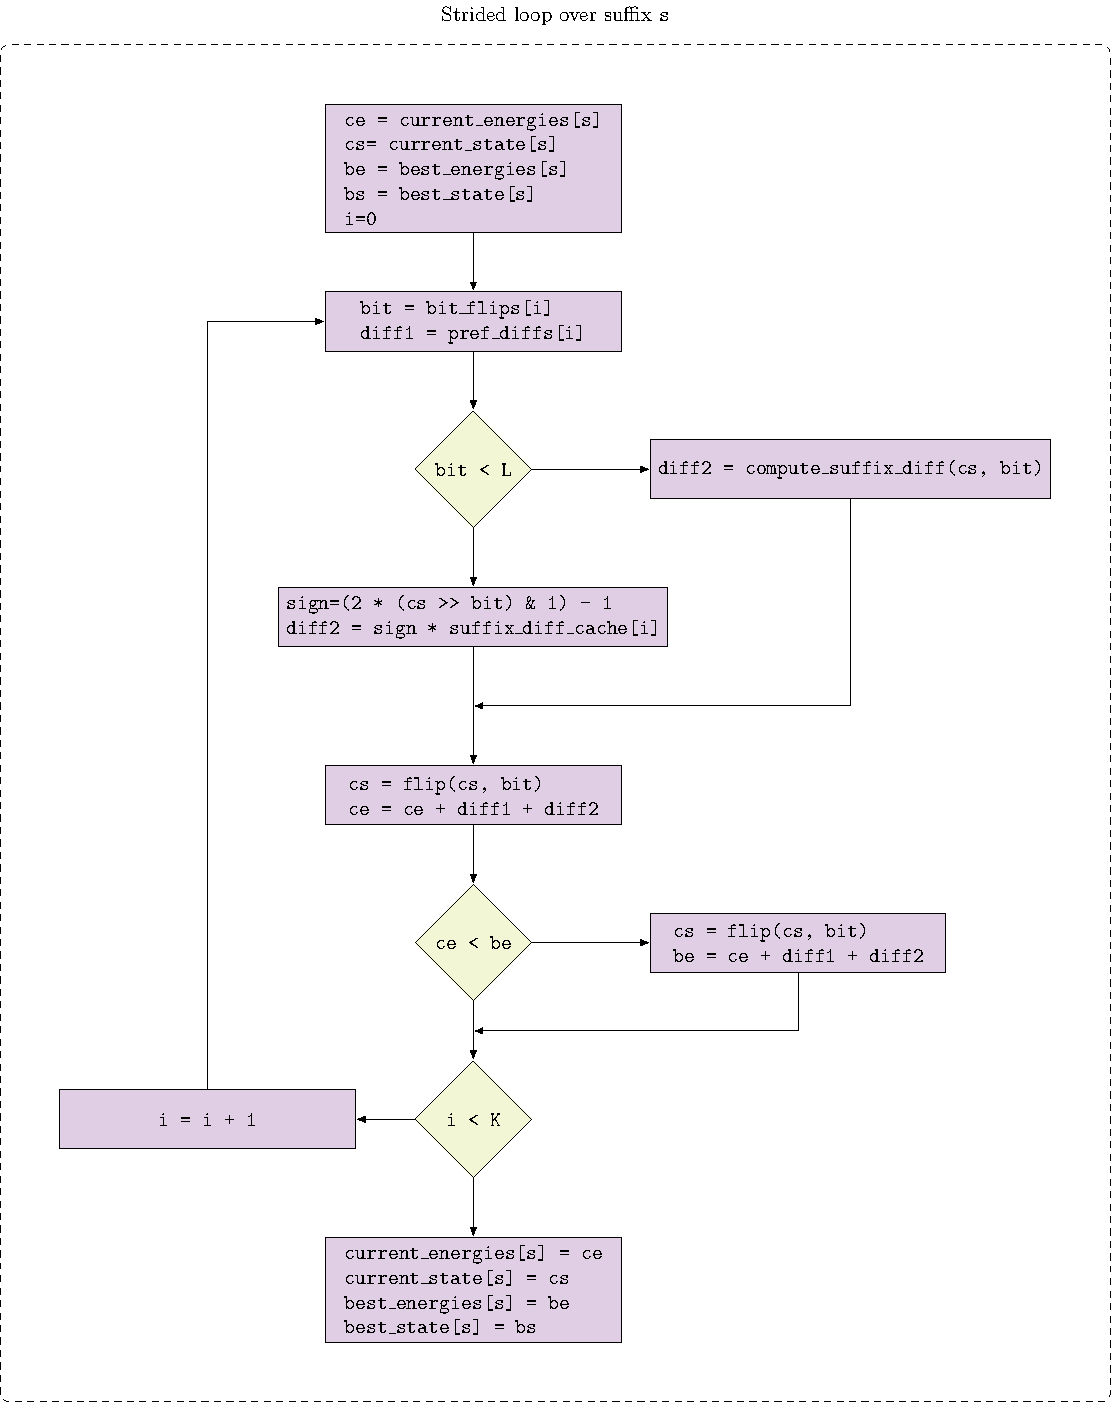
\includegraphics[width=\textwidth]{figures/bruteforcegray2}
  \caption{Implementation of the strided loop for kernel in fig \ref{fig:bruteforcegray}.}
\end{figure}

\subsection{Performance evaluation of the optimized algorithm}

We performed a preliminary performance evaluation of the Gray code--based
algorithm for finding the ground state. For our benchmarks, we used several
setups with different Nvidia GPUs. Some setups were equipped with more than one
copy of the same GPU. The summary of test setups, as well as capabilities of
the used GPUs is presented in table \ref{tab:bruteforce-gs-only-table}.

\begin{table}[!ht]
  \footnotesize
  \begin{tabular}{|l|c|c|c|c|c|}
    \hline
    \cellcolor{theader}                                              & \multicolumn{2}{c|}{\cellcolor{theader} Kernel launch parameters} & \multicolumn{2}{c|}{\cellcolor{theader}Algorithm parameters} & \cellcolor{theader}                                                                      \\
    \hhline{~----~}
    \cellcolor{theader} \multirow{-2}{*}{\cellcolor{theader} GPU(s)} & \cellcolor{tsubheader} Block size                                 & \cellcolor{tsubheader} Grid size                             & \cellcolor{tsubheader} Suffix size & \cellcolor{tsubheader} \makecell{\# Steps per       \\ kernel launch} & \multirow{-2}{*}{\cellcolor{theader} \makecell{\# Fixed \\ variables}}\\
    \hline
    A10                                                              & 512                                                               & 4096                                                         & 27                                 & 4096                                          & N/A \\
    \hline
    A100                                                             & 512                                                               & 4096                                                         & 27                                 & 4096                                          & N/A \\
    \hline
    A6000                                                            & 1024                                                              & 4096                                                         & 27                                 & 4096                                          & N/A \\
    \hline
    V100 x8                                                          & 1024                                                              & 4096                                                         & 27                                 & 4096                                          & 3   \\
    \hline
    DGX H100 x8                                                      & 1024                                                              & 8192                                                         & 29                                 & 8192                                          & 3   \\
    \hline
    RTX 4090 x8                                                      & 512                                                               & 4096                                                         & 28                                 & 4096                                          & 1   \\
    \hline
  \end{tabular}
  \caption{Parameters used for benchmarking} \label{tab:bruteforce-gs-only-table}
\end{table}

Since each of the test setups was available to us only for a limited amount of
time, we were only able to measure execution times for a very limited subset of
parameters, and we needed to make some educated guesses. We decided to use a
constant depth of the prefix differences buffer equal to 10. Depending on the
available memory size, we used suffix sizes of 27, 28 and 29. The tested kernel
executions grids included blocks of 256, 512 or 1024 threads, and 4096 or 8192
blocks per grid. We also considered 2048, 4096 and 8192 algorithm steps per
single kernel execution. The best parameters found for each setup are presented
in table \ref{tab:bruteforce-gs-only-table}. We would like to stress out,
however, that such a coarse--grained process of parameter tuning does not
guarantee their global optimality. Further parameter tuning could be achieved
by searching through a finer grid of parameters, possibly combined with
profiling. Lastly, for multi-GPU setups, we solved each instance by
distributing the work equally between GPUs by splitting the problem into chunks
of equal size. The splitting was done by constructing new QUBOs by fixing the
values of $l$ variables, resulting in $2^{l}$ total subproblems.

The figure Fig. \ref{fig:bruteforce-gsonly-benchmarks} shows the results of our
benchmarks. Observe that for multi-GPU setups and system sizes $N \le 40$, the
execution time is almost constant. This is because the time presented on the
graph factors in the time of scattering work among GPUs and gathering the
results, which for small system sizes dominates the actual solver execution
times. Aside from these plateaus, as expected, the graphs of measured solution
times resemble exponential curves. On the setup with eight DGX H100 GPUs, the
optimized code was able to find the ground state of instances with system size
$N=50$ in less than 5 minutes.

\begin{figure}
  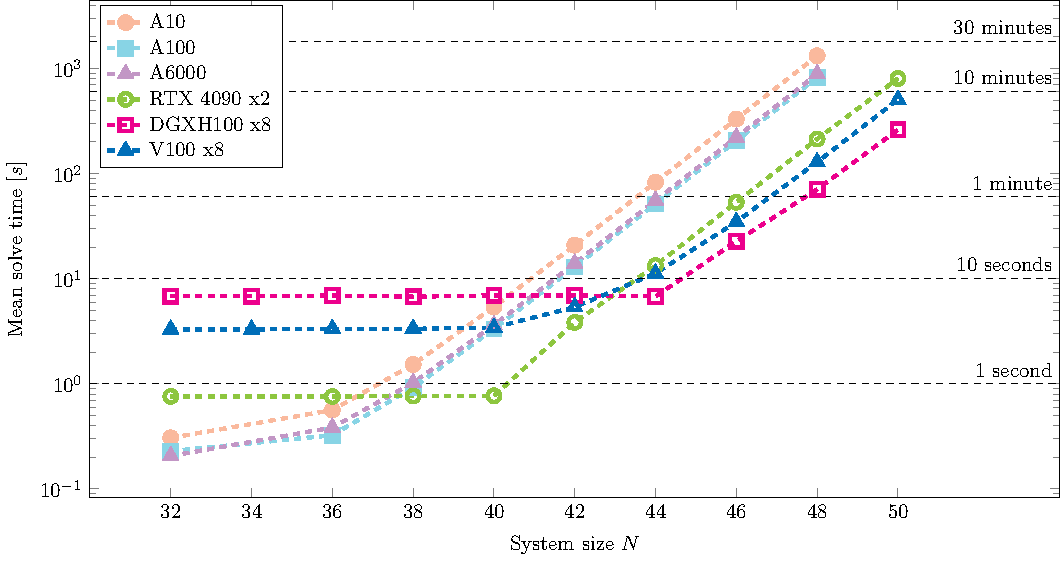
\includegraphics[width=\textwidth]{figures/bf_benchmarks_initial}
  \caption{
    Benchmarking results for Gray code--based brute force algorithm for finding a
    ground state of Ising model. The dashed lines between data points are provided
    for visual guidance. For each system size $N$, the solution times were averaged
    over 20 different instances with known ground states. Observe that for setups
    with multiple GPUs and small system sizes, the solution time remains virtually
    constant. This is because, for small system sizes, the execution time is
    dominated by tasks related to distributing work and gathering results. The
    parameters used for benchmarking in each setup are summarized in table
    \ref{tab:bruteforce-gs-only-table}. } \label{fig:bruteforce-gsonly-benchmarks}
\end{figure}

%%% Local Variables:
%%% mode: latex
%%% TeX-master: "../main"
%%% End:

\chapter[Railway conflict management]{Application to railway conflict management}
\label{chapter:trains}
As the last point in the thesis, in this chapter, we describe how the results
presented so far can be applied in the field of operational research. Namely,
we propose an approach to solving the railway dispatching problem using quantum
annealing. We benchmark the implementation of our algorithm on the current
generation of D-Wave annealers, using solutions obtained via tensor networks
and exhaustive search as a baseline for comparison.

\section{Overview of the problem}
We will consider a part of a railway network, which we will simply refer to as
a \emph{network}. The network is divided into \emph{block sections} or simply
\emph{blocks}. In our approach, we focused only on the single--track railways,
which means that the network can only comprise the following types of blocks:
\begin{itemize}
  \item \emph{Line blocks}, or \emph{single tracks}, sections that can be occupied by one train
    at a time.
  \item \emph{Sidings}, or \emph{parallel tracks} (occurring e.g. at stations). At the sidings,
    trains passing in the same direction can meet--and--overtake (M--O), and trains passing
    in the opposite directions can meet--and--pass (M--P). Each siding comprises two or more
    tracks, each of which can also be occupied by one train at a time. When appropriate, the
    sidings occurring at the stations will be called \emph{station blocks}.
\end{itemize}
Fig. \ref{fig:railway-network} shows an example network.

\begin{figure}[ht]
  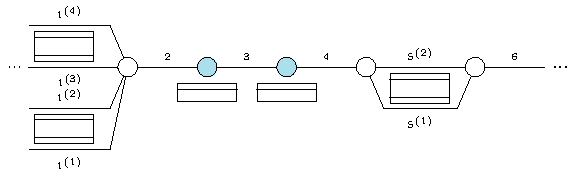
\includegraphics[width=\textwidth]{figures/example_line}
  \caption{
    An example network. Sections $2, 3, 4$ and $6$ are \emph{line blocks}, while
    sections $1$ and $5$ are \emph{sidings} with respectively $4$ and $2$ tracks.
    Rectangles represent platforms. Circles represent points where a line block and
    a siding join (white) or where two line blocks join (blue). Superscripts denote
    tracks within a siding. } \label{fig:railway-network}
\end{figure}

The trains move through the network according to a \emph{timetable}. It is
assumed that this timetable is conflict-free, i.e. at any time no two trains
occupy the same track.

Now, suppose the network is affected by a disturbance, which has prevented some
trains from running according to their original timetable. Examples of possible
disturbances include, but are not limited to, a malfunction of one or more
trains or a malfunction of railway tracks. After the disturbance, some trains
occupy different parts of the networks than they are supposed to and resuming
operations according to the original timetable might not be possible. First of
all, some trains might already be delayed too much to be physically able to
follow the timetable. Secondly, trying to closely follow the timetable after
the disturbance might generate conflicts. The problem might be viewed from
various perspectives, e.g. that of a passenger or transport operation company
\cite{tornquist,lamorgese,Jensen2016}. This this chapter, we look at the
problem of the infrastructure manager whose task, in the presence of a
disturbance, is to create a new, conflict-free timetable. Naturally, in most
cases, there will be multiple possible solutions to the arising conflicts, and
hence one has to decide on what criteria make one timetable more appealing than
another. In our approach, we assume that the dispatcher aims to minimize some
function of the delays, which we will describe later. There are also other
possible choices of the objective function \cite{8795577} such as the total
passenger delay or the total cost of operations.

Let us observe that independently from the algorithm for constructing a new
timetable, some delays after the disturbance might be inevitable, e.g. due to
engineering or even physical limits. For instance, if a train has been broken
for some time, it can only follow the timetable if it is not already late and
it can make up for the time it already lost -- and this can only happen if it
can reach a sufficiently large speed. If this is not the case, the train will
be necessarily delayed. Moreover, by taking into account the maximum speed with
which the trains can move through each section, one can calculate the lower
bounds on how much the train will be delayed at each station. These lower
bounds are known as unavoidable, or \emph{primary}, delays.

In the ideal case, if all the trains could travel at their maximum speed, all
trains would be delayed only by their primary delays and there would be nothing
to optimize. However, it might not always be possible. Suppose for instance,
that two trains going in the same direction are already delayed at a station
neighboring a line block. From each train's perspective, the optimal solution
is to start its route immediately when possible. However, as only one of them
can do this because a line block can only be occupied by one train at a time.
Hence, at least one of these two trains will have a delay larger than the
primary one. What is important is that this additional delay is not a
consequence of some physical or engineering limitations, but rather a
consequence of the dispatcher's decision made to avoid a potential conflict.
All such delays are called the \emph{secondary} delays and, unlike the primary
ones, they are subject to optimization.

The distinction between primary and secondary delays might seem artificial at
first, but it has profound consequences. Namely, when constructing a function
to be minimized we only need to take into account the secondary delays. For
instance, we might want to minimize their total sum or their weighted sum, with
weights corresponding to the trains' priorities.

Our high--level description of the problem needs now a mathematical
formulation. We start by describing the details of the network model in the
next section.

\section{The delay representation}
Before we can formulate the optimization problem to be run on D-Wave, we need
first to formally describe the railway model. The first idea that comes to mind
is to define quantities corresponding to departure and arrival times of each
train and relevant station blocks, and express all other quantities in the
model in terms of their difference with respect to the times found in the
original timetable. However, as we will soon see, one can almost completely
forget about arrival and departure times, and instead express all qunatities in
the model using delays. Moreover, we will further simplify our model by
assuming all secondary delays are integers falling into some finite range.

The set of all trains will be denoted by $\JJ$. This set is naturally
partitioned into the set $\JJ_0$ of trains going into one direction and the set
$\JJ_1$ of trains going into the opposite direction. This is a proper
partition, i.e.:
\begin{equation}
  \JJ_0 \cup \JJ_1 = \JJ \quad \JJ_0 \cap \JJ_1 = \emptyset
\end{equation}
For any train $j \in \JJ$ its route is a sequence of blocks. Our model forbids
recirculation, i.e. each train passes every block in its route exactly once.
Furthermore, we assume that each train starts and ends its route at some
station, and its route is uniquely identified by a sequence of station blocks
$\left(s_{j,1}, s_{j, 2}, \ldots, s_{j, \text{end}_j}\right)$, i.e., there are
no alternative routes between any two stations. For convenience, we will denote
the station block preceding $s_{j,k}$ in a given train's route by
$\pi(s_{j,k})$ and the station block succeeding it by $\rho(s_{j,k})$:
\begin{align}
  \pi(s_{j,k})  & = s_{j,k-1} \quad \mbox{for } 2 \le k \le \mbox{end}_j      \\
  \rho(s_{j,k}) & = s_{j,k+1} \quad \mbox{for } 1 \le k \le \mbox{end}_j - 1.
\end{align}
We will denote the time at which the train $j$ should leave the block $s$
according to the original timetable by $\ttout(j, s)$. Similarly, the time at
which the train $j$ is supposed to leave block $s$ will be denoted by $\ttin(j,
  s)$. In our model, we assume that the time at which a train leaves one block is
precisely the same as the time it enters the next block, i.e.
\begin{equation}
  \ttout(j, s) = \ttin(j, \rho_j(s))
\end{equation}
It is clear that the original timetable determines how long it takes for a
train $j$ to travel through a given block $s$. We call this time the passage
time, denoted by $\pt(j, s)$
\begin{equation}
  \pt(j, s) = \ttout(j, s) - \ttin(j, s)
\end{equation}
An important observation is that passage times defined by the timetable may not
be the minimum physically achievable passing times $\pmin(j, s)$. In other
words, for each train $j$ and block $s$ there exists a time reserve
\begin{equation}
  \label{eq:pt}
  0 \le \alpha(j, s) = \pt(j, s) - \pmin(j, s)
\end{equation}
This time reserve will become important when discussing the propagation of the
primary delays.

\subsection{Delay representation}
Suppose the disturbance happened, resulting in some trains not being able to
meet the schedule. Hence, the actual leaving and arrival times (denoted by
$\tout$ and $\tin$) differ from the scheduled ones. The delay $d(j, s)$ of the
train $j$ at block $s$ is defined as the difference
\begin{equation}
  \label{eq:djs}
  d(j, s) \coloneqq \tout(j, s) - \ttout(j, s) %= \tin(j, \rho(s)) - \ttin(j, \rho(s)).
\end{equation}
As already mentioned, $d(j, s)$ can be expressed as a sum
\begin{equation}
  d(j, s) = d_U(j, s) + d_S(j, s)
\end{equation}
where $d_U$ denotes the primary (or unavoidable) delay, and $d_S$ denotes the
secondary delay. In the absence of time reserve, one would simply have $d_U(j,
  s) = d_U(j, s')$ for a given train $j$ and blocks $s$ and $s'$ on its route.
However, the time reserve allows to somewhat compensate the delays
\begin{equation}
  d_U(j, \rho(s)) = \max\{0, d_U(j, s) - \alpha(j, \rho(s))\}
\end{equation}

The secondary delays can be, in principle, arbitrary large. However, it is
convenient to assume that all secondary delays for the train $j$ are bound from
above by some constant $d_{\max}(j)$. One can find a reasonable upper bound by
running some fast heuristic or determine it manually (e.g. there might be an
\emph{a priori} established maximum allowable delay of the train). Henceforth,
we will consider $d_{\max}(j)$ to be a parameter of the model. With this
assumption, we have the following upper and lower bound on the overall delay
\begin{equation}
  d_U(j, s) \le d(j, s) \le d_U(j, s) + d_{\max}(j).
\end{equation}

\section{Discretizing delays}
Formulation of the problem presented so far can facilitate the construction of
a linear, constrained model of the dispatching problem. However, since the
secondary delay values are continuous variables, such a model would not be
compatible with the quantum annealer. We circumvent this issue by discretizing
the delays. One way to do it is to require that all secondary delays are
natural numbers, i.e.
\begin{equation}
  \forall_{j \in \JJ} \forall_{s \in S_{j}}\quad  d_{s}(j, s) \in \{0, 1, \ldots, d_{\max}(j)\}.
\end{equation}
As a consequence, the total delays get discretized as well. We will denote the
set of possible values for $d(j, s)$ by $A_{j, s}$, i.e.
\begin{equation}
  A_{j, s} \coloneq \{d_{U}(j, s), d_{U}(j, s) + 1, \ldots, d_{U}(j, s) + d_{\max}(j)\}.
\end{equation}
Notice that this discretization is not particularly restrictive, as timetables
typically have a finite resolution of minutes anyway.

We can now use one--hot encoding for $d(j, s)$ and introduce binary variables
$x_{s, j, m}$:

\begin{equation}
  \forall_{j \in \JJ}\forall_{s \in S_{j}} \forall_{m \in A_{j, s}} \quad x_{s,j,m} = \begin{cases}
    1, & d(j, s) = m      \\
    0, & \mbox{otherwise}
  \end{cases}.
\end{equation}
Naturally, possible values for $d(j, s)$ are mutually exclusive, which can be
expressed as the following constraint:
\begin{equation}
  \label{eq:onehotconstraint}
  \forall_{j \in \JJ}\forall_{s \in S_{j}} \sum_{m \in A_{j, s}} x_{s, j, m} = 1
\end{equation}
As for the cost function, we decided to use a simple weighted sum of the
delays, i.e. the cost function of the form
\begin{equation}
  \label{eq:qubo:cost}
  f(\mathbf{x}) = \sum_{j \in \mathcal{J}}\sum_{s \in S^{*}_{j}}\sum_{m \in A_{j,s}} w(s,j,m) \cdot x_{j,s,m},
\end{equation}
For instance, choosing $w(s, j, m)=m$ would result in an objective of
minimizing the sum of all delays. In general, however, one could take into
account the relative importance of the trains, as we will describe later when
introducing the real railway sections considered in our research.

\section{Dispatching conditions}
The cost function \eqref{eq:qubo:cost} together with constraint
\eqref{eq:onehotconstraint} is not enough to construct a meaningful
optimization problem. We also have to take into account other constraints
stemming from dispatching conditions. For instance, we cannot allow a schedule
in which two trains occupy the same track at the same time. We will address
these additional dispatching conditions next.

\subsection{The minimum passing time condition.}
Train cannot travel through a block faster than the corresponding minimum
passing time
\begin{equation}
  \label{eq:dc1}
  \tout(j, s) \ge \tin(j, s) + \pmin(j, s).
\end{equation}
Using \eqref{eq:djs} and \eqref{eq:pt} one can easily verify that inequality
\eqref{eq:dc1} is equivalent to
\begin{equation}
  \label{eq:passingtime}
  d(j, \rho(s)) \ge d(j, s) - \alpha(j, s, \rho(s)).
\end{equation}
In binary variables, it means that if, for a fixed $j,s,m$, the $x_{j,s,m}=1$,
then delays $d(j,s)$ smaller than $m-\alpha(j, s, \rho_j(s))$ are prohibited
and thus the corresponding variables have to zero-out. Hence, we arrive at the
following condition:
\begin{equation}
  \label{eq:qubo:passingtime}
  \forall_{j} \forall_{s \in S_j \setminus \{s_{{j,\text{end}}}\}}
  \sum_{d \in A_{j,s}}
  \left(
  \sum_{ d' \in D(d) \cap A_{j, \rho_j(s)}} x_{j, s, d}
  x_{j, \rho_j(s), d'} \right) = 0,
\end{equation}
where $D(d) = \{0, 1, \ldots, d - \alpha(j, s, \rho_j(s)) -1\}$.
\subsection{The single block occupation condition.}
Two trains cannot occupy the same part of a single railway track. Consider two
trains, $j, j' \in \JJ_0$ leaving the same station $s$ in the direction of the
next station block $\rho_j(s)$. Suppose further that the train $j$ leaves
first. i.e. $\tout(j', s) > \tout(j, s)$. Since two trains cannot occupy the
same block, some amount of time has to pass after $\tout(j, s)$ before the
train $j'$ can leave. This amount of time is dependent on both $j$ and a
sequence of blocks, and hence we denote it by $\tauu(j, s, \rho_j(s))$. Thus,
the condition becomes
\begin{equation}
  \label{eq:single-block}
  \tout(j', s) \ge \tout(j, s) + \tauu(j, s, \rho_j(s)).
\end{equation}
Substituting for $\tout$ in \eqref{eq:single-block} yields the following
inequality for delays
\begin{equation}
  \label{eq:single-block-delays}
  d(j', s) \ge d(j, s) + \ttout(j, s) - \ttout(j', s) + \tauu(j, s, \rho_j(s))
\end{equation}
or,
\begin{equation}
  d(j', s) \ge d(j, s) + \Delta(j, s, j', s) + \tauu(j, s, \rho_j(s))
\end{equation}
where
\begin{equation}
  \label{eq:delta}
  \Delta(j, s, j', s) = \ttout(j, s) - \ttout(j', s)
\end{equation}
The precise form of $\tauu$ depends on the dispatching detail of the problem.
In our approach, we propose the following form:
\begin{equation}
  \tauu(j, s) = \max_{i \in \{k+1,\ldots,l-1\}}(\ttin(j, m_{i+1}) - \ttin(j, m_i))
\end{equation}

For our decision variables, we use a similar scheme as with the previous
constraint, and the condition becomes:
\begin{equation}
  \label{eq:qubo:singleblock}
  \forall_{i=0,1} \forall_{j, j' \in \JJ^{i}} \forall_{s \in S^{*}_{j} \cap S^{*}_{j'}} \sum_{m \in A_{j, s}} \left(
  \sum_{m' \in B(m) \cap A_{j', s}} x_{j,s,m}x_{j',s,m'}
  \right) = 0,
\end{equation}
where $B(m) = \{m + \Delta(j, s, j', s), d + \Delta(j, s, j', s)+ 1,\ldots, m +
    \Delta(j, s, j', s) + \tau_{(1)}(j,s, \rho_j(s))-1 \}$ is a set of delays
violating condition \eqref{eq:single-block-delays}.

\subsection{The deadlock condition}
The deadlock condition is analogous to the single block occupation condition
but for trains going in opposite directions. Suppose trains $j$ and $j'$ are
heading in opposite directions on a route determined by two consecutive
stations $s$ and $\rho_j(s)$. Note that for $j'$ the order is reversed, i.e. it
starts at $\rho_j(s)$ and travels in the direction of $s$. In this case, $j$
has to arrive at $\rho_j(s)$ before $j'$ can leave $\rho_j(s)$. We formalize it
as:
\begin{equation}
  \label{eq:deadlock}
  \tout(j', \rho_j(s)) \ge \tout(j,s) + \tauuu(j, s, \rho_j(s)),
\end{equation}
where $\tauuu(j, s, \rho_j(s))$ is the minimum time required for train $j$ to
get from station block $s$ to $\rho_{j}(s)$. Rewritten in terms of delays, the
inequality \eqref{eq:deadlock} reads:
\begin{equation}
  \label{eq:deadlock2}
  d(j',\rho_j(s)) \ge d(j, s) + \Delta(j,s,j',\rho_j(s)) + \tauuu(j, s, \rho_j(s)).
\end{equation}
This condition is to be applied for pairs of trains $j,j'$ going in opposite
dimension if train $j$ is supposed to leave before the train $j'$ leaves
$\rho_{j}(s)$, otherwise the order has to be appropriately reversed.

In decision variables, the deadlock condition in its basic form looks as
follows
\begin{equation}
  \label{eq:qubo:deadlock}
  \forall_{s \in S^{*}_{j} \cap S^{*}_{j'}} \sum_{m \in A_{j, s}} \left(
  \sum_{m' \in C(m) \cap A_{j', s}} x_{j,s,m}x_{j',s,m'}
  \right) = 0,
\end{equation}
and has to be applied for limited number of trains $j \in \JJ^{0} (\JJ^{1})$
and $j' \in \JJ^{1}(\JJ^{0})$. This limit is imposed indirectly by the upper
bounds on the delays. Here, $C(m)$ is, similarly to $B(m)$, the set of delays
violating the condition for the given pair.
\subsection{The rolling stock circulation condition}
Our model assumes that some trains are assigned the same train set. Naturally,
there exists some necessary \emph{turnover time}, before a train set can be
used. Formally, if trains $j$ and $j'$ going in opposite directions are
assigned the same train set, then the following inequality has to hold:
\begin{equation}
  \tout(j', s_{j',1}) > \tout(j, s_{j,end}) + \Delta(j, j')
\end{equation}
where $\Delta(j, j')$ is the minimum turnover time. In the delay
representation, the inequality becomes:
\begin{equation}
  \label{eq:rolling}
  \begin{split}
    d(j',s_{j',1}) + \ttout(j',s_{j',1}) > & \; d(j, s_{j,end-1}) + \ttout(j, s_{j,end-1}) + \\
    & \; \tauuu(j, s_{j,end-1}) + \Delta(j,j').
  \end{split}
\end{equation}
Inequality \eqref{eq:rolling} can be simplified to
\begin{equation}
  d(j',s_{j',1}) > d(j, s_{j,end-1}) - R(j,j'),
\end{equation}
by setting
\begin{equation}
  \label{eq:rolling2}
  R(j, j') = \ttout(j',s_{j',1}) - \ttout(j, s_{j,end-1}) - \tauuu(j,s_{j,end-1})
\end{equation}
In decision variables, the rolling stock circulation condition for trains $j$
and $j'$ can be written as
\begin{equation}
  \label{eq:qubo:rollingstock}
  \sum_{m \in A_{j, s_{(j, end-1)}}} \sum_{m' \in E(d) \cap A_{j',s_{(j',1)}}} x_{j,s_{(j,end-1)},m}x_{j', s_{(j',1)},m'} = 0
\end{equation}
where $E(d) = \{0, 1, \ldots, m-R(j, j')\}$.

\subsection{Penalties}
The conditions \eqref{eq:qubo:passingtime}, \eqref{eq:qubo:singleblock},
\eqref{eq:qubo:deadlock}, \eqref{eq:qubo:rollingstock} together with cost
function \eqref{eq:qubo:cost} define a constrained $0-1$ problem. However, in
order to use a quantum annealer, we must convert it to QUBO, which means we
have to incorporate those constraints into the cost function.

One might observe that penalties defined by the dispatching conditions are of
the form:
\begin{equation}
  \label{eq:quadraticpenalty}
  \sum_{(j, j') \in \mathcal{V}_{p}} x_{i}x_{j} = 0,
\end{equation}
for some set of pairs of indices $\mathcal{V}_{p}$. For every feasible solution
(i.e. one meeting all the constraints) the sum in equation
\eqref{eq:quadraticpenalty} is 0, whereas violation of the corresponding
condition gives a strictly positive value. Hence, one can add such a sum to the
cost function, effectively penalizing the infeasible solutions. More generally,
one might multiply the sum by some constant $\ppair > 0$, to further increase
the value of the cost function for the infeasible solutions.

The same reasoning cannot be applied e.g. to the constraint
\eqref{eq:onehotconstraint}, which comprises equations of the form
\begin{equation}
  \label{eq:linearpenalty}
  \sum_{i \in \mathcal{V}_{s}}x_{i} = 1.
\end{equation}
If one added sums from the equation \eqref{eq:linearpenalty} to the cost
function, it would favor the infeasible solution comprising of all 0s. Instead,
one can consider the following quadratic form of the same penalty:
\begin{equation}
  \label{eq:linearpenalty2}
  \left(\sum_{i \in \mathcal{V}_{s}}x_{i} -1 \right)^{2} = 0
\end{equation}
In contrast to \eqref{eq:linearpenalty}, this time the left hand is equal to 0
for feasible solution, and a positive value for any solution violating the
one--hot encoding constraint. As with previous, quadratic penalties, we might
want to multiply such penalties by some constant $\psum > 0$. An important
thing to mention here is that the expansion of the left-hand side in
\eqref{eq:linearpenalty2} gives a nonzero constant offset, which we will
ignore. therefore, the final form of the penalty term reads:
\begin{equation}
  \mathcal{P}_{sum}(\mathbf{x}) = \sum_{\mathcal{V}_{s}}p_{sum}\left(\sum_{i,j \in \mathcal{V}_{s}^{\times 2}, i\ne j} x_{i}x_{j}  - \sum_{i \in \mathcal{V}_{s}}x_{i}\right).
\end{equation}
Lastly, the total cost function for our QUBO reads:
\begin{equation}
  f'(\mathbf{x}) = f(\mathbf{x}) + \mathcal{P}_{sum}(\mathbf{x}) + \mathcal{P}_{pair}(\mathbf{x}).
\end{equation}
\section{Results}

\subsection{Studied railway segments}
In our work, we considered two single-track railway lines managed by the polish
state--owned company PKP Polskie Linie Kolejowe:

\begin{itemize}
  \item Railway line No. 216 (Nidzica -- Olsztynek section)
  \item Railway line No. 191 (Goleszów -- Wisła Uzdrowisko section)
\end{itemize}

The segments are depicted in Fig. \ref{fig:linesmall:line} and Fig.
\ref{fig:linelarge:line}. For the railway line No. 216, we considered its
official train schedule (as of April 2020). The line No. 191 was undergoing a
renovation at the time of writing, and hence it had no available timetable.
Based on the planned parameters of the line, as described in the official
documents \cite{PKPPLK}, we constructed a cyclic timetable. Initial,
undisturbed timetables are depicted in Fig. \ref{fig:linesmall:diagram} and
Fig. \ref{fig:linelarge:diagram}.

\begin{figure}
  \begin{subfigure}{\textwidth}
    \caption{}\label{fig:linesmall:line}
    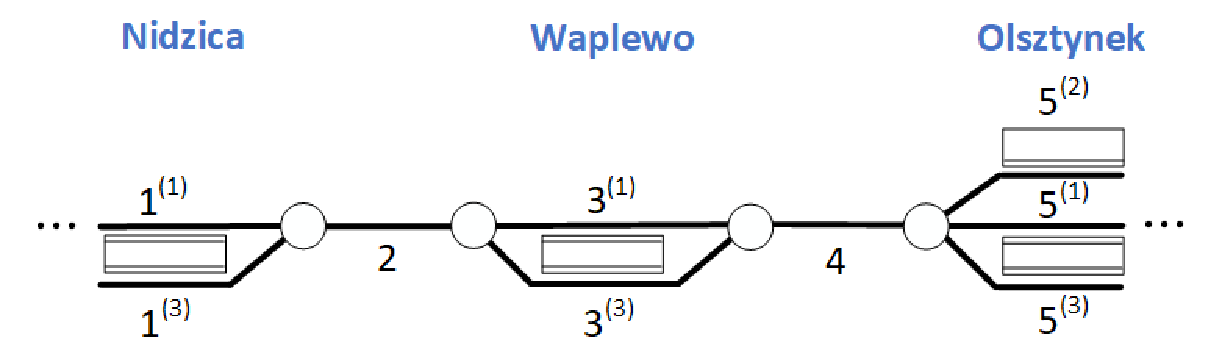
\includegraphics[width=\textwidth]{figures/line_small.pdf}
  \end{subfigure}
  \begin{subfigure}{\textwidth}
    \caption{}\label{fig:linesmall:diagram}
    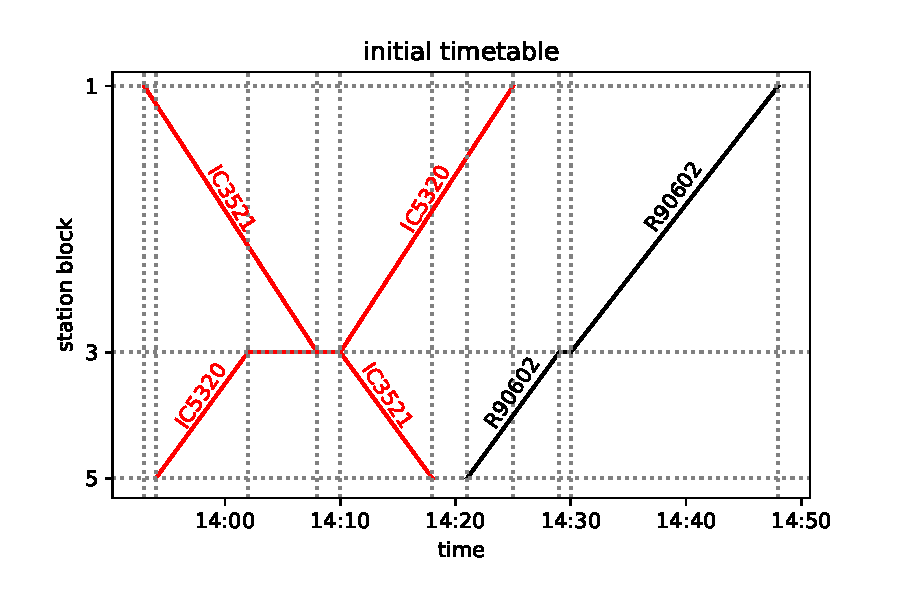
\includegraphics[width=\textwidth]{figures/train_diagram_small}
  \end{subfigure}
  \caption{\subref{fig:linesmall:line} Nidzica -- Olsztynek segment of line No. 216. The segment comprises three
    station blocks (1 -- Nidzica, 3 -- Waplewo, 5 -- Olsztynek), and two line
    blocks (2, 4). We assume that passing through the station block takes the same
    amount of time independently of which track is used. \subref{fig:linesmall:diagram} Train diagram for the undisturbed timetable of the line in \subref{fig:linesmall:line}. The timetable features two
    \emph{Inter--City} trains IC3521 and IC3520 and one \emph{Regio} train R90602. The paths for the
    \emph{Inter-City} trains are marked with red and path of the \emph{Regio} train is marked with black.}
  \label{fig:linesmall}
\end{figure}

\begin{figure}
  \begin{subfigure}{\textwidth}
    \caption{}\label{fig:linelarge:line}
    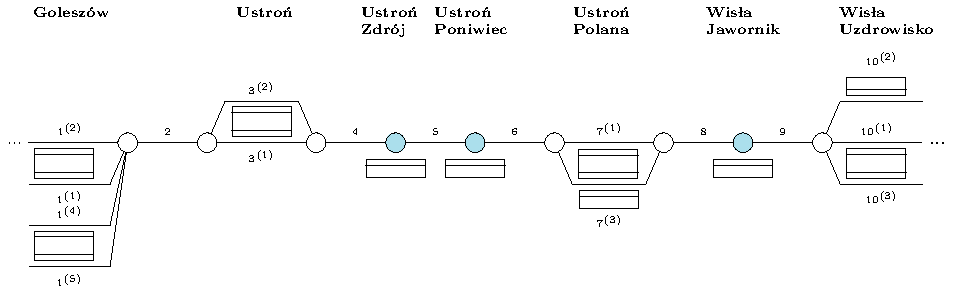
\includegraphics[width=\textwidth]{figures/line.pdf}
  \end{subfigure}
  \begin{subfigure}{\textwidth}
    \caption{}\label{fig:linelarge:diagram}
    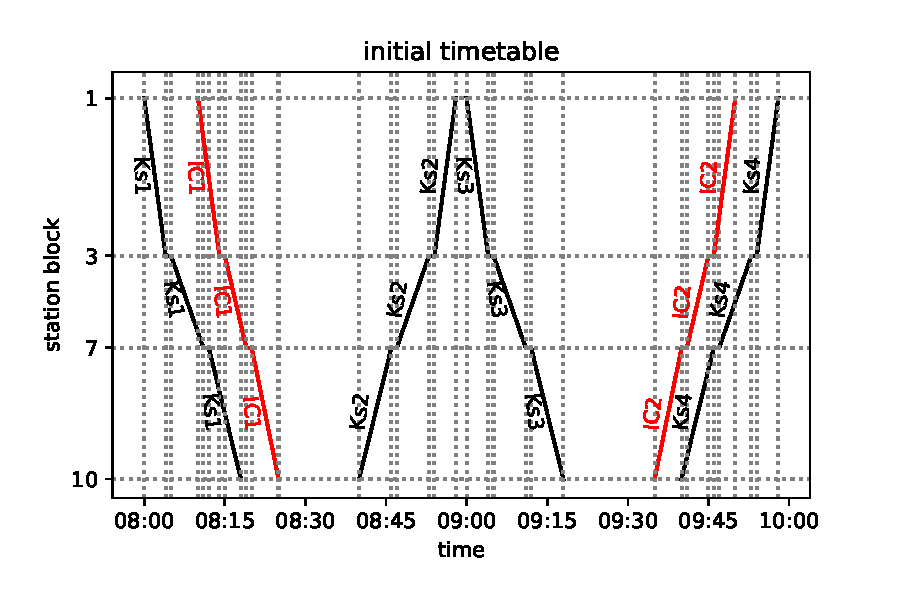
\includegraphics[width=\textwidth]{figures/train_diagram}
  \end{subfigure}
  \caption{\subref{fig:linelarge:line} Goleszów -- Wisła Uzdrowisko segment of line No. 191. The segment comprises 4
    station blocks (1 -- Goleszów, 3 -- Ustroń, 7 -- Ustroń Polana, 10 -- Wisła
    Uzdrowisko) and 6 line blocks (2, 4, 5, 6, 8, 9). Between line blocks there are
    additional passenger platforms at Ustroń Zdrój, Ustroń Poniwiec and Wisła
    Jawornik. \subref{fig:linelarge:diagram} Train diagram for the timetable of the line in \subref{fig:linelarge:line}.
    The timetable features two \emph{Inter--City} trains (IC1 and IC2) and four regional trains (Ks1--Ks4).
    The paths of the \emph{Inter--City} trains are marked with red and paths of the regional trains are
    marked with black.}
  \label{fig:linelarge}
\end{figure}

Timetable for the network segment of line No. 216 includes two
\emph{Inter-City} trains, IC5320 and IC3521, and a regional \emph{Regio} train
R90602. For the line No. 191, the timetable includes two \emph{Inter-City}
trains IC1, IC2 and four regional trains Ks1--Ks4. We assume both
\emph{Inter-City} trains in line No. 191 are operated with the same train set,
with a minimum service time of $R(j,j') = 20\mbox{minutes}$.

For both network segments, we assume that the minimum waiting times at all
considered stations are 1 minute. Also, we assume that the passing times
through all the line blocks were initially scheduled according to the maximum
permissible speeds. As a result of those assumptions, the only possible nonzero
time reserve occurs at the station blocks.

\subsection{Disturbance scenarios}

For the Nidzica--Olsztynek railway segment, we considered a single scenario
with two delays. The purpose of this scenario is to illustrate our approach on
a simple and yet real-world example. The first one is a 15-minute delay of
IC5320 starting from station block 5. The second one is that of the IC3521
leaving station block 1 5 minutes late. Considering this and our assumptions,
this creates conflicts, where two \emph{Inter--City} trains, as well as an
\emph{Inter--City} train and the \emph{Regio} train, have conflicts at block 4.
The conflicted, infeasible train diagram for this situation is depicted in Fig.
\ref{fig:smallconflict}.

\begin{figure}
  \begin{subfigure}[b]{0.5\columnwidth}
    \caption{}\label{conflict}
    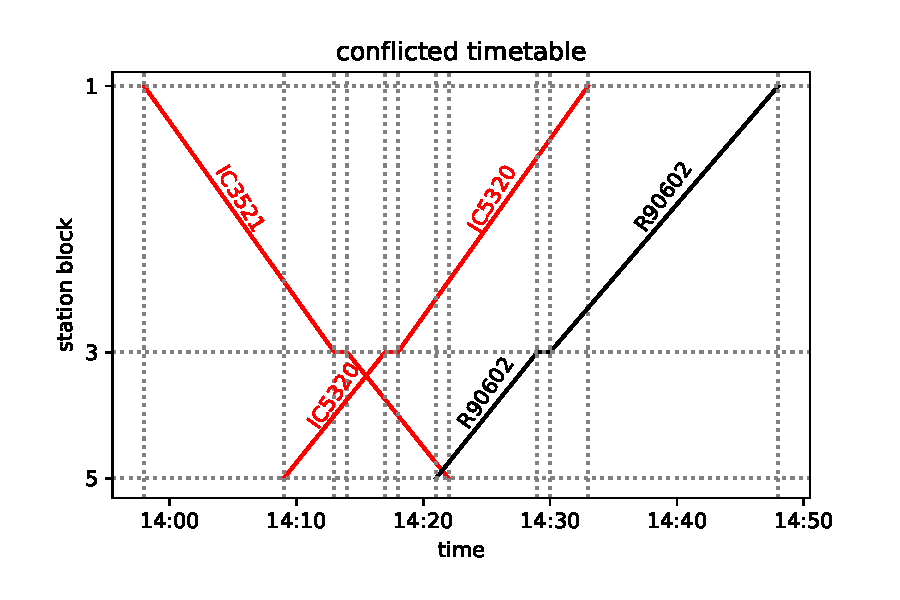
\includegraphics[width=\textwidth]{figures/small_conflict}
  \end{subfigure}
  \begin{subfigure}[b]{0.5\columnwidth}
    \caption{}\label{resolution}
    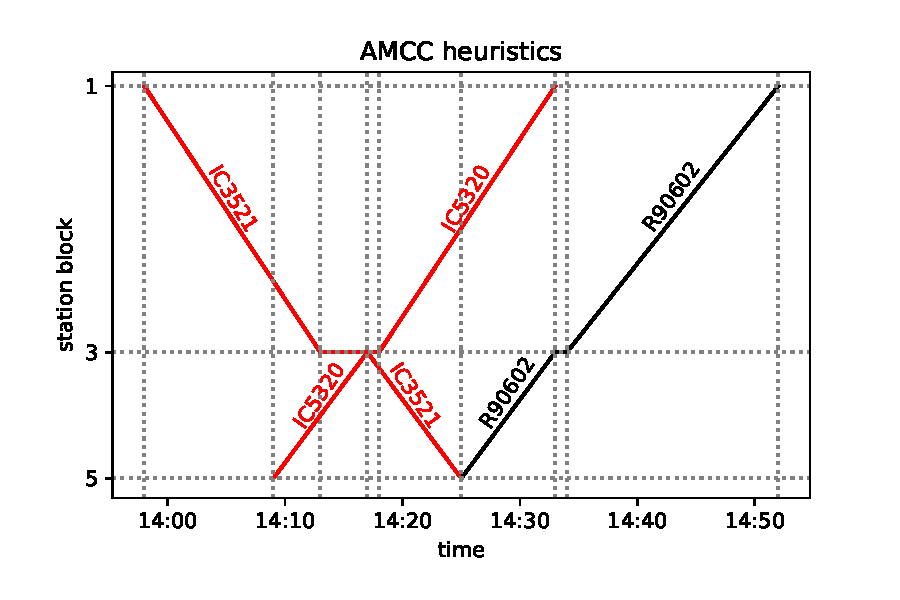
\includegraphics[width=\textwidth]{figures/small_solution}
  \end{subfigure}
  \caption{
    \subref{conflict} Conflicted timetable for railway segment of line No. 216. Compared to the original timetable
    (Fig. \ref{fig:linesmall:diagram}), two trains are delayed, resulting in two conflicts. The conflicts
    can be quickly identified visually as intersections of train paths at line blocks.
    \subref{resolution} Conflict resolution via AMCC heuristics. The same solution was obtained using FCFS and FLFS heuristics.
  }
  \label{fig:smallconflict}
\end{figure}

For the Goleszów -- Wisła Uzdrowisko line, we considered several different
scenarios, which were designed to illustrate our approach on a larger example:

\begin{enumerate}
  \item A moderate delay of the \emph{Inter--City} train starting from the station
    block 1. This results in a single conflict between IC1 and Ks2.
  \item A moderate delay of all the trains starting from station block 1, resulting in
    two conflicts.
  \item A significant delay of some trains starting from station block 1. Results in
    two conflicts.
  \item A significant delay of the \emph{Inter--City} train IC1 starting from the
    station block 1. Results in a single conflict, which is straightforward to
    resolve.
\end{enumerate}

The delays in all the aforementioned scenarios were chosen so that they indeed
result in conflicts. The conflicted timetables are presented in Fig.
\ref{fig:conflictlarge}.

\begin{figure}
  \begin{subfigure}[b]{0.5\textwidth}
    \caption{}\label{c1}
    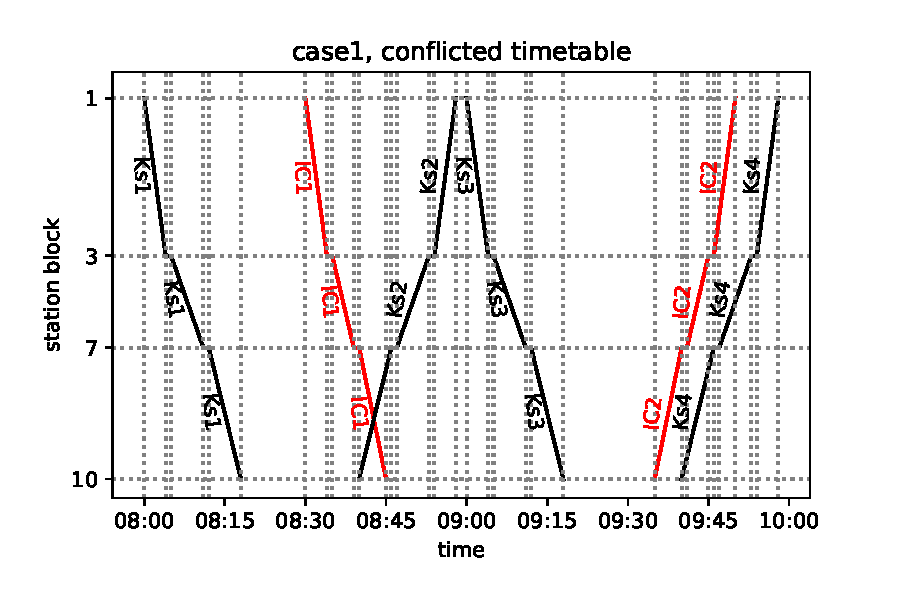
\includegraphics[width=\textwidth]{figures/case1_conflict}
  \end{subfigure}
  \begin{subfigure}[b]{0.5\textwidth}
    \caption{}\label{c2}
    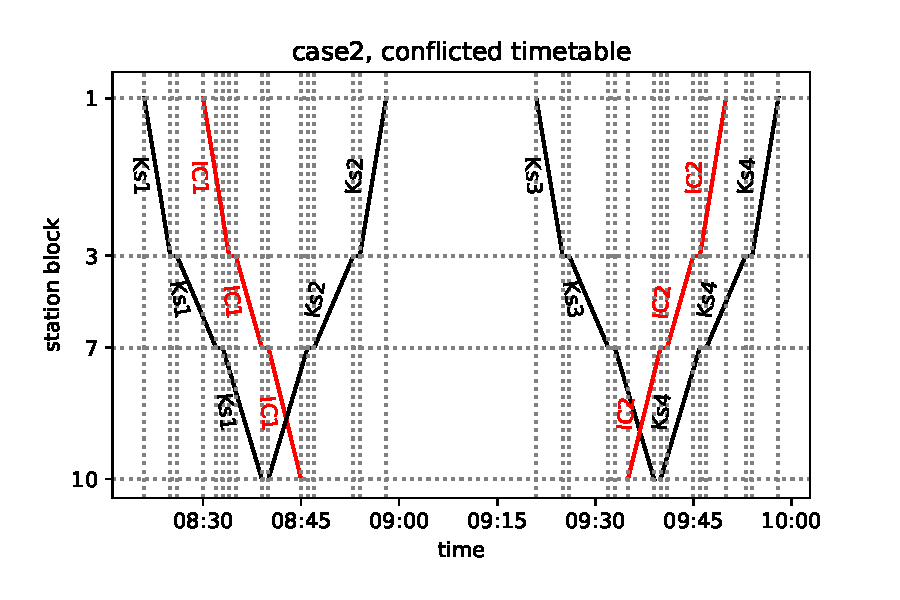
\includegraphics[width=\textwidth]{figures/case2_conflict}
  \end{subfigure}

  \begin{subfigure}[b]{0.5\textwidth}
    \caption{} \label{c3}
    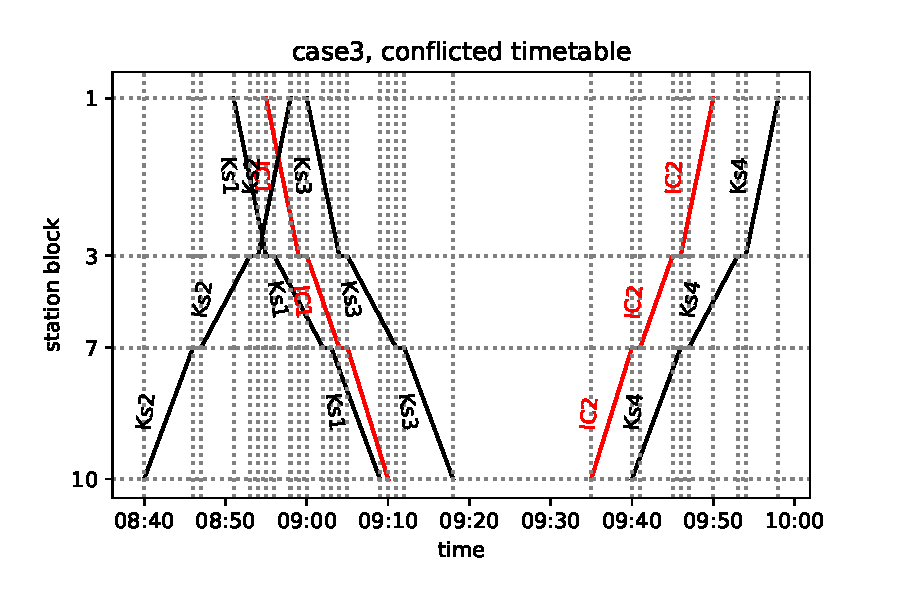
\includegraphics[width=\textwidth]{figures/case3_conflict}
  \end{subfigure}
  \begin{subfigure}[b]{0.5\textwidth}
    \caption{}\label{c4}
    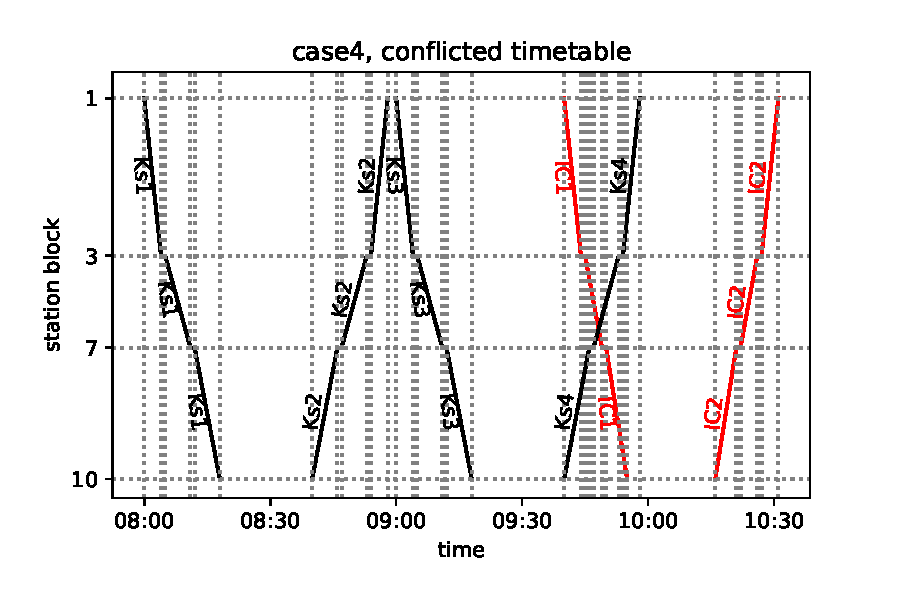
\includegraphics[width=\textwidth]{figures/case4_conflict}
  \end{subfigure}
  \caption{Conflicted timetables for line No. 216. \subref{c1} Single conflict, observe
    that the additional delay of Ks$2$ will propagate to the delay of Ks$3$.
    \subref{c2} Two conflicts, with no impact of Ks$2$ on Ks$3$. \subref{c3}
    Multiple conflicts. \subref{c4} One conflict, straightforward to resolve.}
  \label{fig:conflictlarge}
\end{figure}

\subsection{Solution using simple heuristics}
To establish a baseline for Quantum Annealing, we solved the problems described
in the previous section using simple heuristics common in the railways
practice. Those heuristics are:

\begin{itemize}
  \item FCFS (First Come First Served),
  \item FLFS (First Leave First Served),
  \item AMCC (Avoid Maximum Current $C_{\max}$.
\end{itemize}

In FCFS (resp. FLFS) the way is given to the train that first arrives (resp.
first leaves) the considered station block at which the conflict occurs. AMCC
\cite{mascis2002job} is slightly more complex. In this heuristic, one tries to
minimize the maximum secondary delays of the trains. We want to stress that
those heuristics facilitate different objective functions, and hence it is not
possible to directly compare them -- nevertheless, it might be useful to
discuss qualitative differences between the solutions they produce. The
solutions provided by the AMCC heuristic also provide a lower bound for the
values of maximum secondary delays $d_{\max}(j)$, which we will use when
constructing QUBO.

For the case of Nidzica--Olsztynek line, all heuristics returned the same
solution, depicted in Fig. \ref{resolution}. The conflict is avoided by
delaying IC3521 by another 3-minutes, and allowing R9062 to enter the block not
earlier than 14:25, i.e. 4 minutes later than in the conflicted timetable. In
this case, the additional 4 minutes constitute the maximum secondary delay of
the solution.

We also applied the aforementioned heuristics to all the considered
disturbances in the Goleszów -- Wisła Uzdrowisko segment. For brevity, we
refrain from presenting a detailed discussion of the solutions for all the
cases and limit ourselves to the summary of the maximum secondary delay, which
is presented in Table \ref{tab:simple}

\begin{table}[bh]
  \centering
  \begin{tabular}{|c|c|c|c|c|}
    \hline
    \rowcolor{theader} Heuristics & case $1$ & case $2$ & case $3$ & case $4$ \\
    \hline
    FLFS                          & 6        & 13       & 4        & 2        \\
    \hline
    FCFS                          & 5        & 5        & 5        & 2        \\
    \hline
    AMCC                          & 5        & 5        & 4        & 2        \\
    \hline
  \end{tabular}
  \caption{The maximum secondary delays, in minutes, resulting from simple heuristics.
    Observe that for each case, there are solutions far below $d_{\text{max}} =
      10$.} \label{tab:simple}
\end{table}

\subsection{Details on QUBO construction}

To formulate our dispatching problems as QUBO and solve them on the D-Wave
annealer (or using any other method), we first need to decide on the values of
several parameters of the model, as well as the precise form of the cost
function. We start with the latter.

We decided on using the cost function proportional to the secondary delays of
all trains entering their last station block. Additionally, we weight the
contributions of each delay with a coefficient depending on the prioritization
of the corresponding train, resulting in the cost function of the form:
\begin{equation}
  f(\mathbf{x}) = \sum_{j \in J}\left(\sum_{m  \in A_{j,s^{*}}}w_{j} \frac{d(j,s^{*}) - d_{U}(j,s^{*})}{d_{\max}(j)}x_{j,s^{*},m}\right),
\end{equation}
where $s^{*} = s_{j,end-1}$. The priorities $w_{j}$ are chosen specifically for
both networks. One can immediately observe that larger values of $w_{j}$
increase contribution stemming from the delay of a given train, and hence the
objective function favors solutions with smaller delays for the trains with
larger priorities. For the segment of line No. 216, we assume $w_{j}= 1.5$ for
all \emph{Inter-City} trains, and the $w_{j}=1.0$ for the regional train. This
prioritization coincides with the usual prioritization of trains in Poland (and
many countries). For the segment of line No. 191, we decided to adopt a
slightly more complicated prioritization. For the trains heading toward block
10, we set a lower priority of $w_{j}=0.9$. For the trains heading in the
opposite direction, we set $w_{j}=1.5$ and $w_{j}=1.0$ for \emph{Inter-City}
and regional trains respectively. This is because the trains heading towards
block 1 (Goleszów) also head towards important junctions in Polish railway
network (Katowice for regional trains, and capital city of Warsaw for
\emph{Inter-city} trains). Our strategy therefore tries to avoid larger delays
in this direction to limit further disturbance to the rest of the network.

As for the maximum secondary delay $d_{\max}$, for simplicity, we assume it is
the same for all trains. On the one hand, its value cannot be smaller than the
one returned by the AMCC heuristics. On the other hand, setting this value too
high increases the number of decision variables and complicates the objective
function, which is especially undesirable because of the limited number of
qubits on D-Wave annealers. For line No. 216, we set $d_{\max}=7$ and for line
No. 191 we set $d_{\max}=10$. The total number of decision variables is given
by
\begin{equation}
  \mbox{\#variables} = (\mbox{\#station blocks}-1) \cdot (\mbox{\#number of trains}) \cdot (d_{\max}+1)
\end{equation}
We therefore get $2\cdot 3 \cdot 8 = 48$ decision variables for line No. 216
and $3 \cdot 6 \cdot 11 = 198$ variables for line No. 191. Importantly, the
moderately low number of variables for line no. 216 allows us to solve it using
the brute--force algorithm presented in Chapter \ref{chapter:bruteforce}.

Lastly, we need to choose values for $p_{pair}$ and $p_{sum}$ penalty weights.
This is a very subtle choice. On the one hand, setting it too low may cause
some of the infeasible solutions to have the value of the objective function
smaller than that of feasible solutions, which is undesirable. On the other
hand, if penalty weights are too high, the actual cost function becomes merely
a perturbation for the penalty terms, which is also undesirable. To illustrate
the difference those weights make to the energy landscape, we computed the
low-energy spectrum for the problem defined on line No. 216 for several
different values of $p_{pair}$ and $p_{sum}$. The histograms of energies
obtained in this way are presented in Fig. \ref{fig:penaltyhistogram}.

\begin{figure}
  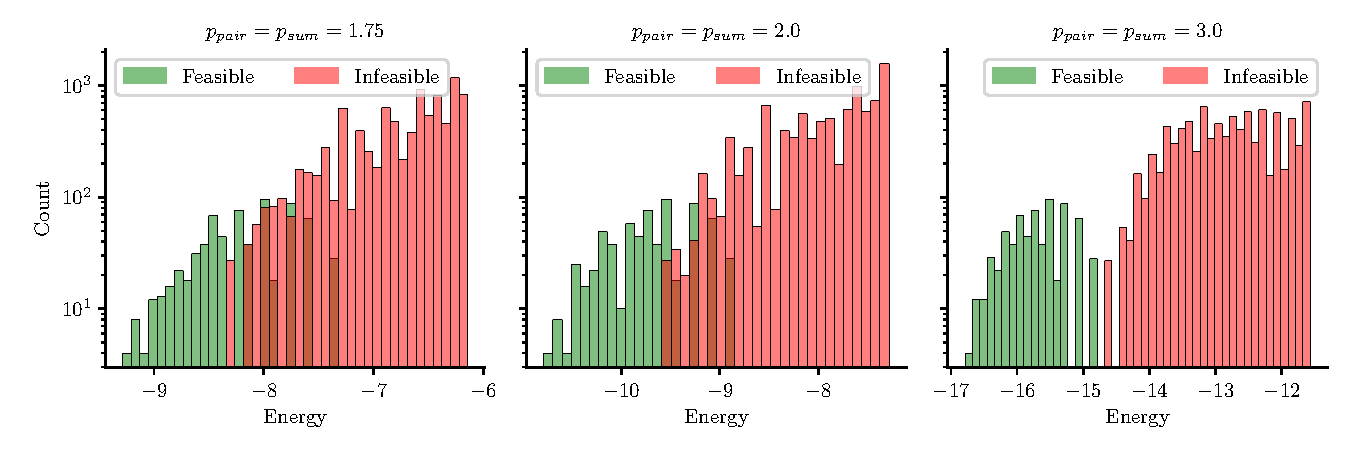
\includegraphics[width=\textwidth]{figures/railway_histograms_bf}
  \caption{Energy histogram for feasible (green) and infeasible (red) solutions of QUBO
    defined for line No. 216 with varying penalty weights. The figure takes into
    account the first 5000 low-energy states.} \label{fig:penaltyhistogram}
\end{figure}
In our experiments, we used several combinations of $p_{pair}$ and $p_{sum}$.
For D-Wave 2000Q series devices, which we used for the experiments reported
in~\cite{railwaydispatching}, we used $p_{\text{pair}}=2.7$,
$p_{\text{sum}}=2.2$ and $p_{\text{pair}} = p_{\text{sum}} = 1.75$.
Additionally, in this thesis, we extend these results by running additional
experiments with $p_{\text{pair}}=p_{\text{sum}}=n$ for $n=2, 3, 4$ on
Advantage and Advantage2 prototype devices.

\subsubsection{Initial experiments on D-Wave annealers}
In our initial experiments, reported in \cite{railwaydispatching}, we used
mostly the D-Wave 2000Q device. We were able to successfully embed all the
problem instances, except case 3 for Line 191. As for the QUBO parameters, we
used $p_{\text{pair}}=2.2$, $p_{\text{sum}}=2.7$ and
$p_{\text{pair}}=p_{\text{sum}}=1.75$. We used several values of the chain
strengths, all of them being a multiplicity of $\max|J_{ij}|$ (computed
separately for each problem before the embedding). Following convention from
\cite{railwaydispatching}, we call the multiplier \emph{chain strength scale}
($css$), and in our experiments, it ranged from $1$ to $9$. The annealing time
varied between $5$--$2000\mu$s.

For QUBO defined for Line 216, the D-Wave annealers failed to reach the ground
state for all the tested parameters. However, the lowest energy--solution found
by the annealer was equivalent to the ground state from the dispatching
perspective\footnote{Here, equivalent from the dispatching perspective means
  that the order of trains leaving any given station is the same.).}. The Fig.
\ref{fig:dwtrainsold} shows the solutions obtained from the D-Wave annealer, as
well as the deviation from the ground state energy. Since the best solution was
obtained for $css=2$, we decided to use the same value for the consecutive
experiments.

\begin{figure}
  \begin{subfigure}[b]{0.5\textwidth}
    \caption{}\label{fig:dwtd1}
    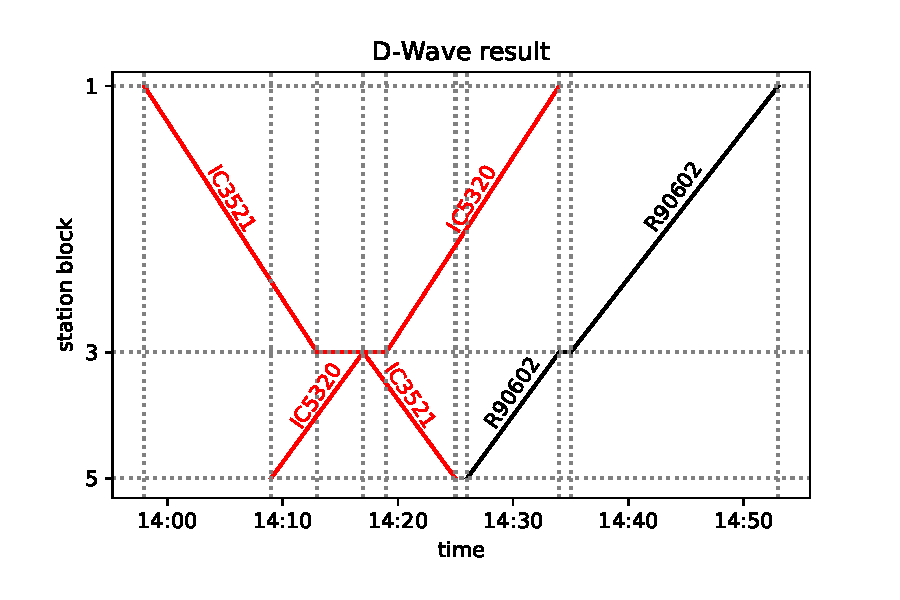
\includegraphics[width=\textwidth]{figures/small_DWave22_27_2000_2}
  \end{subfigure}
  \begin{subfigure}[b]{0.5\textwidth}
    \caption{}\label{fig:dwtd2}
    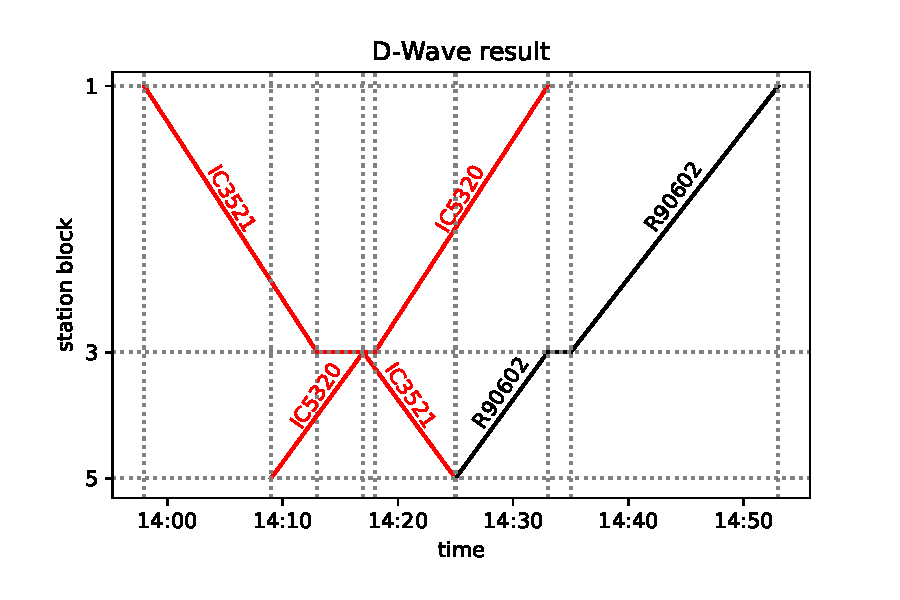
\includegraphics[width=\textwidth]{figures/small_DWave175_175_2000_2}
  \end{subfigure}
  \begin{subfigure}[b]{0.5\textwidth}
    \caption{}\label{fig:dwen1}
    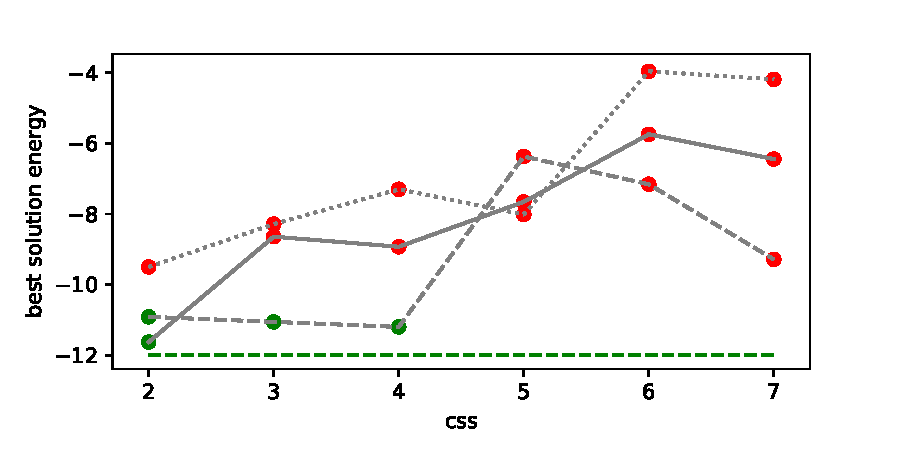
\includegraphics[width=\textwidth]{figures/energy_small_22_27}
  \end{subfigure}
  \begin{subfigure}[b]{0.5\textwidth}
    \caption{}\label{fig:dwen2}
    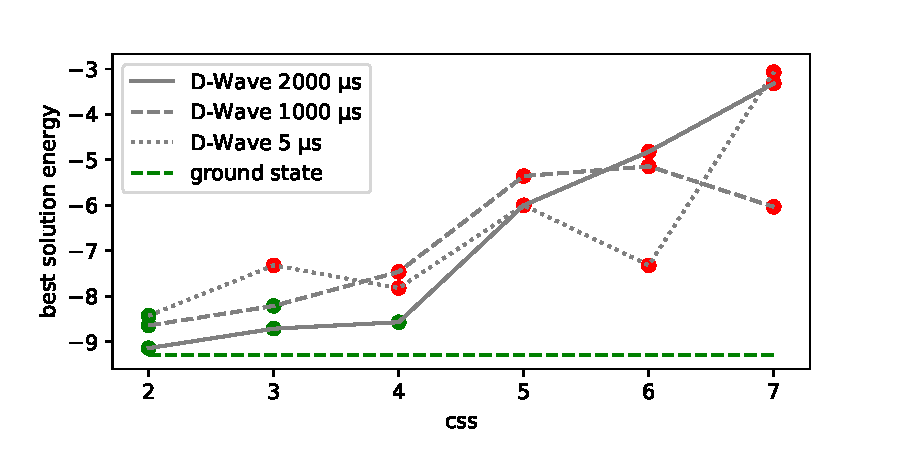
\includegraphics[width=\textwidth]{figures/energy_small_175_175}
  \end{subfigure}
  \caption{
    \textbf{a.} -- \textbf{b.} Best solutions obtained with D-Wave 2000Q annealer,
    optimized over all annealing times and chain strength scales.
    \textbf{c.} -- \textbf{d.} Energy of the best D-Wave solution as the function of
    $css$ scale. For panels \textbf{a.} and \textbf{c.} we used $\ppair=2.2$, $\psum=2.7$
    and for panels \textbf{b}, \textbf{d.} we used $\ppair=1.75$, $\psum=1.75$.
  }
  \label{fig:dwtrainsold}
\end{figure}

Finding a feasible solution for QUBOs defined for Line 191 proved to be much
more difficult for the D-Wave 2000Q annealer. Hence, we increased the total
number of obtained samples to $250$k. Still, even with the increased number of
samples we were unable to reach a feasible solution. The best solutions found
by the annealer for case 1 and case 2 violate a single constraint and can be
easily corrected to obtain a feasible (and in case 2, even optimal) solution,
see Fig. \ref{fig:dwtrainsoldlarge}.

\begin{figure}
  \begin{subfigure}[b]{0.5\textwidth}
    \caption{}\label{fig:dwtd1}
    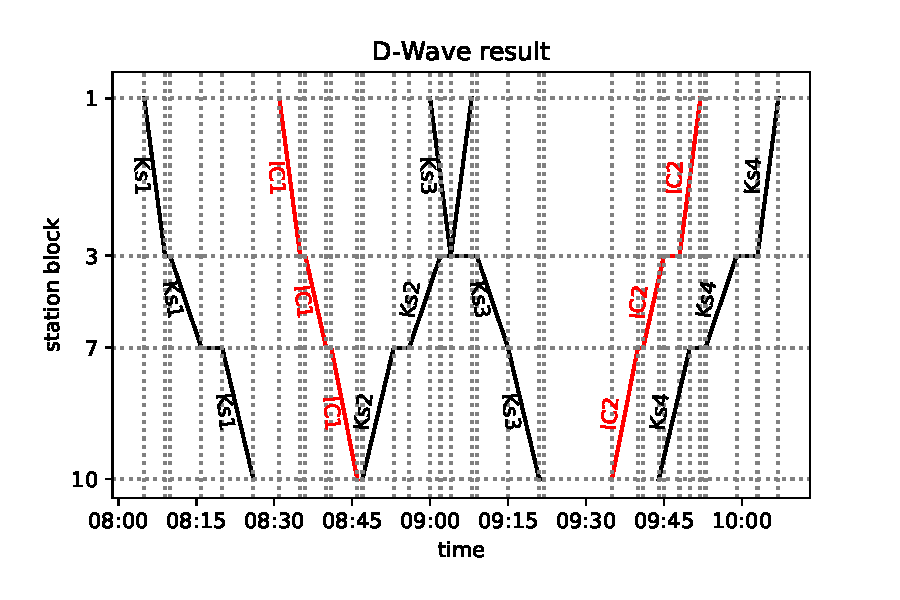
\includegraphics[width=\textwidth]{figures/sol_case1_DWave_1400_2_250k}
  \end{subfigure}
  \begin{subfigure}[b]{0.5\textwidth}
    \caption{}\label{fig:dwtd2}
    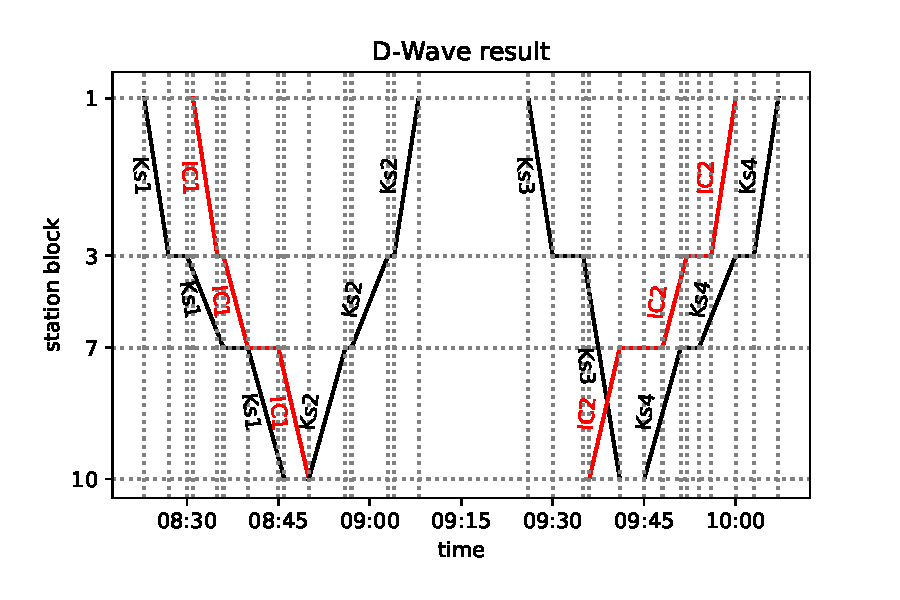
\includegraphics[width=\textwidth]{figures/sol_case2_DWave_1200_2_250k}
  \end{subfigure}
  \caption{
    Lowest energy solutions obtained for QUBO problems defined for Line 191. In all
    panels $\ppair = 2.2, \psum = 2.7$ and $css=2.0$. \textbf{a.} Solution obtained
    for case 1 (with annealing time $\tau=1400$). The solution is infeasible
    because the train Ks3 stays at the station block 7 shorter than 1 minute. The
    solution can be turned into a feasible one by prolonging the stay of Ks3 at
    station block 7. \textbf{b.} The best solution obtained for case 2
    ($\tau=1200$). The solution is infeasible as Ks3 does not stop at station 7.
    This solution can be made into an optimal one by shortening the stays of Ks3 at
    station 3 and IC2 at station 7. } \label{fig:dwtrainsoldlarge}
\end{figure}

In comparison, the QUBOs for cases 1--4 turn out to not be that challenging for
the classical solvers. Both the tensor networks algorithm, described in chapter
\ref{chapter:tn}, and the IBM CPLEX solver were able to find high-quality
solutions equivalent to the ground state from the dispatching point of view,
with CPLEX slightly outperforming the tensor network algorithm in cases 3 and
4. The values of the cost function obtained from these solvers are presented in
table \ref{tab:line191classical}. In the same table, we also present, for
reference, values of our objective function for solutions obtained with simple
heuristics.

At the time we were conducting experiments presented in
\cite{railwaydispatching}, the new Advantage System 1.1 device was entering the
market, and we were able to run a very limited set of experiments. We decided
to try a slightly larger problem, constructed by extending the timetable for
Line 191 with more trains. Although we were able to embed it on the device, our
attempts to find a feasible solution on this early Pegasus-based system were
futile. For the details of this part of the experiment, we refer the interested
reader to \cite{railwaydispatching}.

\begin{table}
  \centering
  \begin{tabular}{|c|c|c|c|c|c|}
    \hline
    \rowcolor{theader} \multicolumn{2}{|c|}{Method} & Case 1          & Case 2                      & Case 3                      & Case 4                                                    \\
    \hline
    \multirow{2}{*}{QUBO model}                     & CPLEX           & \textcolor{RoyalBlue}{0.54} & \textcolor{RoyalBlue}{1.40} & \textcolor{RoyalBlue}{0.73} & \textcolor{RoyalBlue}{0.20} \\
    \cline{2-6}
                                                    & Tensor Networks & \textcolor{RoyalBlue}{0.54} & \textcolor{RoyalBlue}{1.40} & \textcolor{RoyalBlue}{1.65} & \textcolor{RoyalBlue}{0.29} \\
    \hline
    \multirow{3}{*}{Simple heuristics}              & AMCC            & 0.77                        & \textcolor{RoyalBlue}{1.30} & \textcolor{RoyalBlue}{0.73} & \textcolor{RoyalBlue}{0.20} \\
    \cline{2-6}
                                                    & FLFS            & \textcolor{RoyalBlue}{0.54} & 1.71                        & \textcolor{RoyalBlue}{0.73} & \textcolor{RoyalBlue}{0.20} \\
    \cline{2-6}
                                                    & FCFS            & 0.77                        & \textcolor{RoyalBlue}{1.30} & 0.95                        & \textcolor{RoyalBlue}{0.20} \\
    \hline
  \end{tabular}
  \caption{
    Values of the cost functions obtained by the classical solvers for the QUBO
    problems defined for line 191. Values marked with \textcolor{RoyalBlue}{blue}
    represent solutions equivalent (from the dispatching perspective) to the ground
    state of the corresponding problem. Values for the solutions obtained with
    simple heuristics are provided for reference, but it should be noted that those
    methods use different objective functions and hence cannot be directly compared
    to CPLEX or tensor networks-based solver. } \label{tab:line191classical}
\end{table}

\subsubsection{Extended experiment on the Advantage System annealers}

Since the time of our experiments described in the previous section, new models
of the annealers from the Advantage System generation became available.
Furthermore, the first Advantage2 Prototype devices entered the market. We
decided to extend our experiment and run further tests to investigate the
performance of these devices for a broader range of parameters. To this end, we
decided to test how the newer Pegasus-based devices perform on the QUBO problem
defined on Line 216. We decided that due to the limitation of our resources, we
could not run comprehensive experiments with the problem cases defined on Line
191, and instead opted for a more comprehensive sweep through the parameter
space for the smaller problem.

In this new scenario, we decided to increase $\ppair$ and $\psum$ values, to
investigate if a wider energy separation between feasible and infeasible
solutions will be beneficial for the annealers' performance. As previously, the
annealing times varied from $\tau=5$ to $\tau=2000$. We used chain strengths
varying between $4$ and $12$. We would like to stress, that here we mean
absolute values of the chain strengths and not scales of chain strengths in
relation to the maximum absolute value of quadratic terms of the problem like
in the initial experiment.

All of the annealers were able to find a feasible solution to the problem for
at least some combination of parameters. However, their performance varied
highly depending on the parameter range. The frequency of finding a feasible
solution by the annealers is depicted in Fig. \ref{fig:dwline216freq}. As seen
there, the Advantage System6.3 and Advantage2 Prototype1.1 devices exhibited
much better performance than the older Advantage System4.1 device. As for the
quality of the solutions, all solvers managed to find an optimal solution,
although with different frequencies. The summary of parameters for which a
ground state was obtained is presented in table \ref{tab:line216ground}.
Example ground states found are depicted in Fig. \ref{fig:dwline216grounds}.

\begin{table}
  \small
  \centering
  \begin{tabular}{|c|c|c|c|}
    \hline
    \rowcolor{theader} Solver & chain strength & annealing time & \# occurrences \\
    \hline
    Advantage System4.1       & 10             & 200            & 1              \\
    \hline
    Advantage System4.1       & 12             & 500            & 1              \\
    \hline
    \hline
    Advantage System6.3       & 10             & 500            & 1              \\
    \hline
    Advantage System6.3       & 12             & 100            & 1              \\
    \hline
    \hline
    Advantage2 Prototype1.1   & 12             & 5              & 1              \\
    \hline
    Advantage2 Prototype1.1   & 12             & 100            & 3              \\
    \hline
    Advantage2 Prototype1.1   & 12             & 1000           & 4              \\
    \hline
    Advantage2 Prototype1.1   & 12             & 2000           & 1              \\
    \hline
  \end{tabular}
  \caption{Parameters for which D-Wave annealer managed to find the optimal solution to
    the problem defined on Line 216. All ground states occurred at
    $p_{\text{pair}}=p_{\text{sum}}=4.0$. } \label{tab:line216ground}
\end{table}

\begin{figure}
  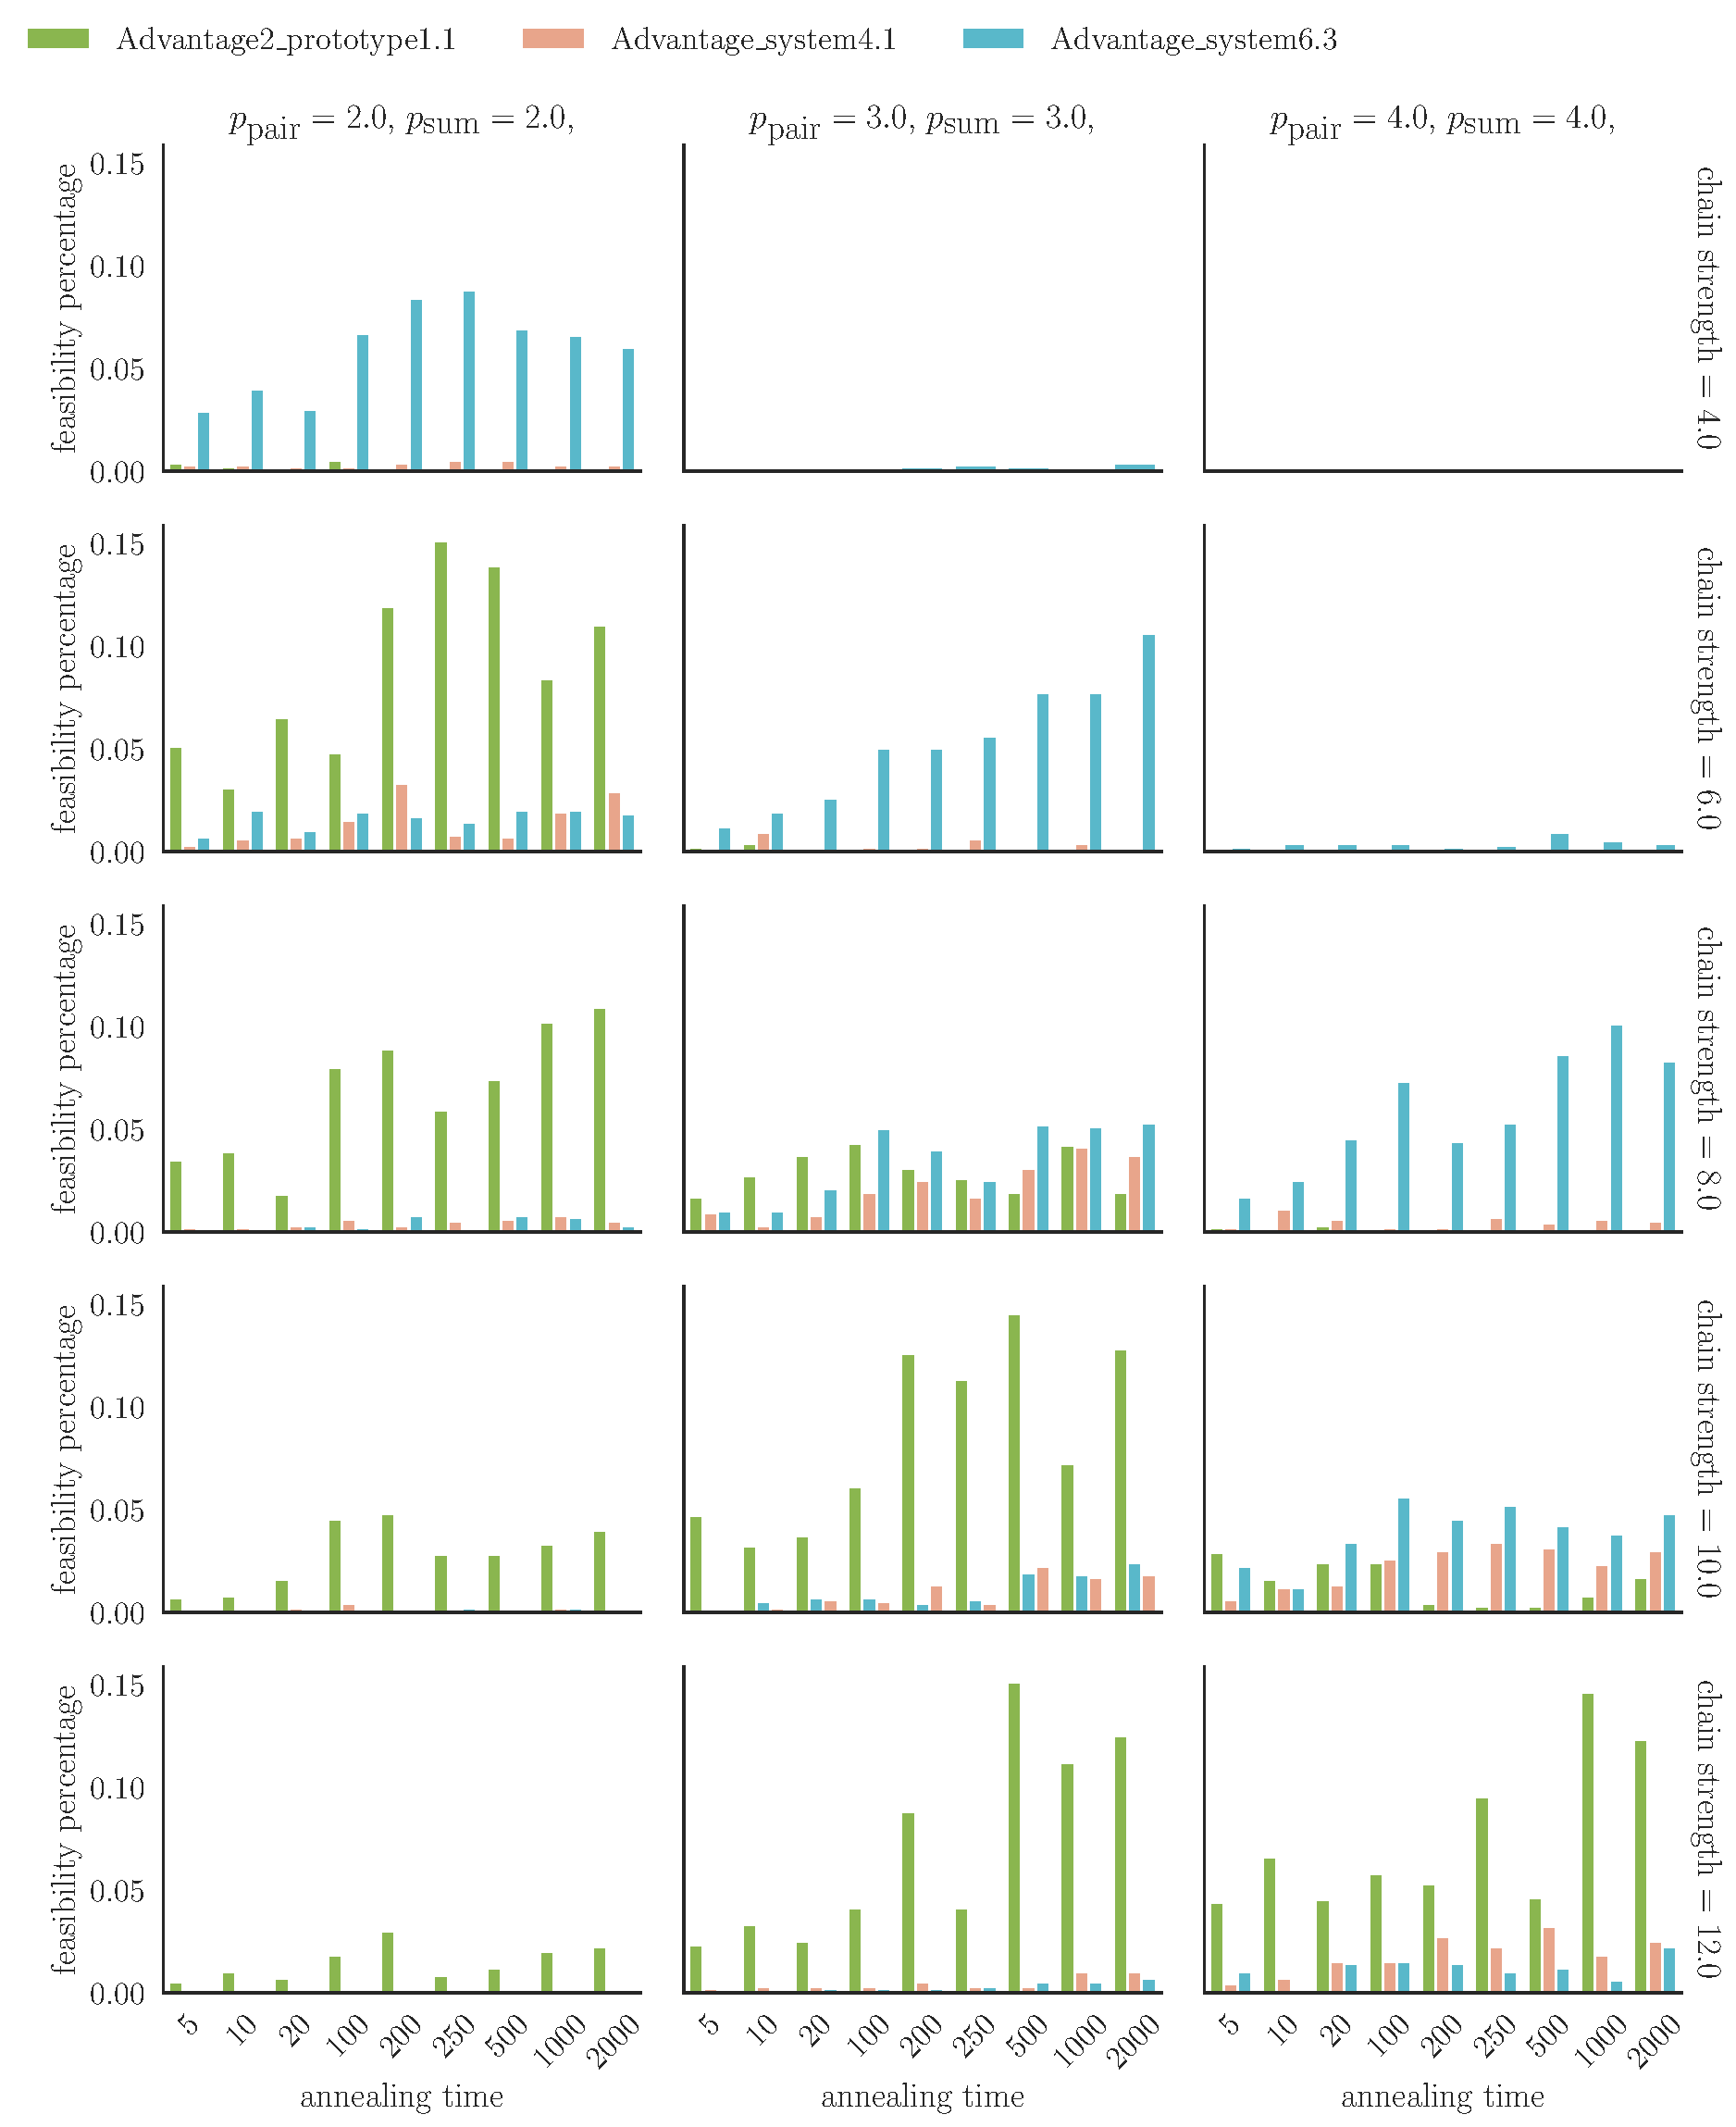
\includegraphics[width=\textwidth]{figures/dwave_line_216_result.pdf}
  \caption{
    Frequency of finding a feasible solution for the problem defined for Line 216.
    Rows in the grid correspond to different values of chain strength and the
    columns correspond to different values of penalty scalings. In each cell, the
    X-axis depicts the annealing time $\tau$, while the $Y$-axis depicts the
    obtained fraction of the feasible solution (out of 1000 samples) }
  \label{fig:dwline216freq}
\end{figure}

One of the interesting observations one could make about the results presented
in Fig. \ref{fig:dwline216freq} is the performance difference between different
models of the annealers, which seem to be highly dependent on the regime of
parameters. Determining the sources of these differences requires further
research, but it is possible that they can be partially explained by
differences in the available range of quadratic coefficients between the
devices (see D-Wave QPU datasheets \cite{dwavedocs}), which in turn might
affect the DAC quantization effect (see discussion of error sources in section
\ref{sec:parallel-in-time}).

\begin{figure}
  \begin{subfigure}[b]{0.5\textwidth}
    \caption{}\label{c1}
    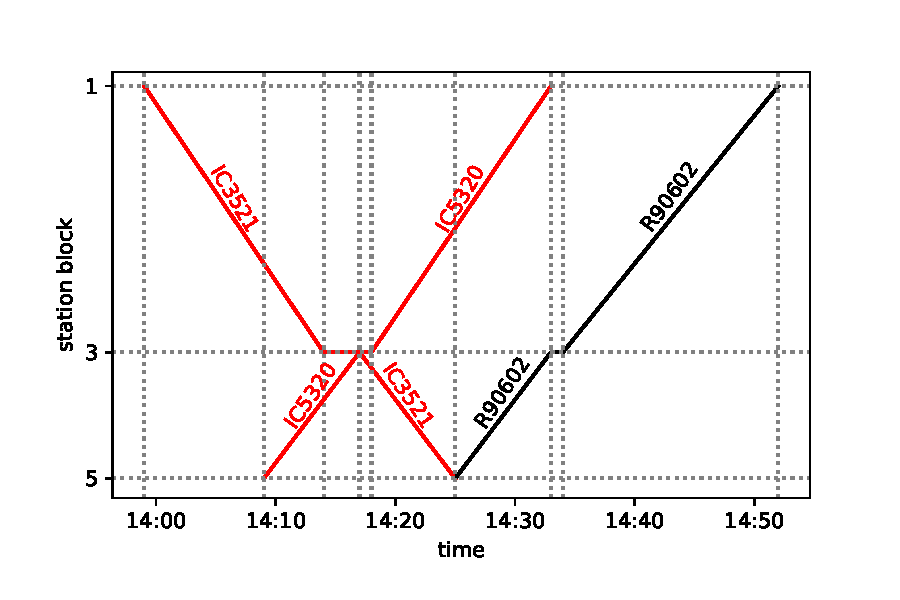
\includegraphics[width=\textwidth]{figures/dwave_line216_ground1}
  \end{subfigure}
  \begin{subfigure}[b]{0.5\textwidth}
    \caption{}\label{c2}
    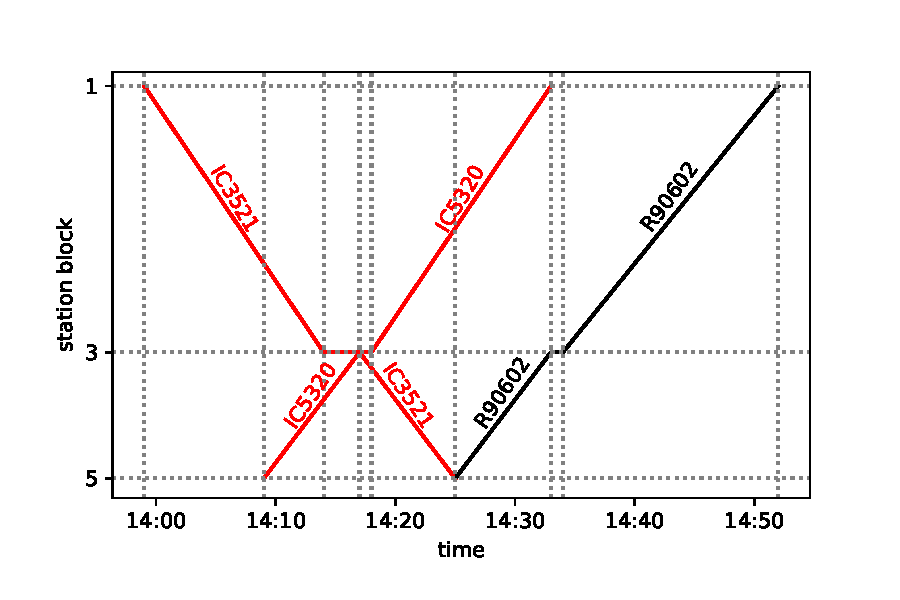
\includegraphics[width=\textwidth]{figures/dwave_line216_ground1.pdf}
  \end{subfigure}
  \caption{Example ground state solutions for the conflicted timetable of Line 216. All
    other ground states are equivalent from the dispatching point of view.}
  \label{fig:dwline216grounds}
\end{figure}

%%% Local Variables:
%%% mode: pdflatex
%%% TeX-master: "../main"
%%% End:

\chapter*{Summary}

In this thesis, we focused on benchmarking quantum annealers and validating their
usefulness in practical settings. One of the most anticipated uses of quantum computers
is simulating physics, or, more precisely, simulating the dynamics of quantum systems.
Therefore, it seems there is no better benchmark for a quantum computer than to test
how far it is from achieving this long--awaited goal. To this end, we described in detail a
proof-of-concept algorithm for simulating the dynamics of a quantum (or in fact, any
dynamical) system using quantum annealers. Although the applicability of the algorithm
to current devices is limited by their small number of qubits and sparse connectivity,
our experiments indicated that already the present-day D-Wave annealers can capture
the dynamics of a very simple two-level system. We also contrasted the obtained results
with the ones produced by several classical solvers, concluding that they perform better
than the tested quantum devices. We also provided a possible explanation why the
particular optimization problems solved in our experiments are particularly hard for
D-Wave devices and checked our predictions with numerical experiments.

To assist in the process of benchmarking the annealers, we developed two distinctive
algorithms. The recent, tensor network-based algorithm allows one to solve Ising
spin--glass instances defined on Chimera graph and other similar layouts. The algorithm
is useful in itself as an optimization approach, but for other research conducted for
this thesis, provided a classical baseline for the results obtained by the D-Wave
annealer. The second of our algorithms, a massively parallelizable distributed brute-force
algorithm, allows for the exact computation of the low--energy spectrum of small,
but otherwise arbitrary, spin-glass instances. Importantly, this simple yet
efficient algorithm is exact and deterministic. We used the brute-force algorithm
to obtain low-energy spectra for some of the smaller instances used throughout
our experiments. This provided us not only with a means of assessing the quality of
solutions obtained from other solvers or annealers but also with valuable
insights into the structure of the solution space.

To benchmark another anticipated use of quantum annealers, i.e. solving hard
optimization problems stemming from real-life problems, we described an approach
for solving railway-dispatching problems by converting them to QUBO. We then
conducted experiments testing our approach on two generations of D-Wave quantum
annealers. Remarkably, for our tests, we used real railway timetables from two Polish
railway segments. In our experiments, D-Wave annealers were able to successfully
find an optimal solution to the small problem instances, although the performance
varied greatly depending on the parameters such as the annealing time and chain strength.

%%% Local Variables:
%%% mode: latex
%%% TeX-master: "../main"
%%% End:



\printbibliography

\appendix
\chapter{Asymptotic notation}

In order to characterize the complexity of algorithms, it is useful to use
asymptotic big-O notation. Consider two functions $f, g \colon \NN \to \RR$. We
say that $f$ is $O(g)$ if and only if there exists a constant $C > 0$ and a
natural number $n_{C}$ such that the inequality $0 \le f(n) \le C\cdot g(n)$
holds for all $n > n_{C}$ \cite{clrs}. It is common to write $f=O(g)$ instead
of ``$f$ is $O(g)$'', slightly abusing the mathematical notation \cite{clrs}.
One should notice that big-O notation does not provide a tight bound. For
instance, we have $n + 1 = O(n)$ (since $n + 1 \le 2 \cdot n$) but also $n+1 =
  O(n^{10})$.

In the context of computational complexity, big-O notation is most commonly
used for expressing upper bound on number of (dominating) operations performed
by an algorithm as a function of its input size $N$. Since the number of
performed operations is roughly proportional to the algorithm's execution time,
it follows that algorithms with better bound can be considered as more
performant. However, care must be taken when applying this reasoning to judge
practical performance. In particular, one should be mindful of the constant
factor $C$ in the definition above, as well as any bottlenecks stemming from
the working of the underlying hardware. As a concrete example, Strassen's
algorithm for multiplying two $N \times N$ matrices requires $O(N^{\alpha})$
multiplications, where $2 < \alpha < 3$, and yet may perform worse than naive
algorithm peforming $N^{3}$ multiplications, even for $N$ of order of several
hundreds \cite{dalberto}.

We conclude this section by mentioning that there exist several other
asymptotic notations. For instance, $\Omega$, describing asymptotic lower bound
of a function, and $\Theta$ combining big-O and $\Theta$. For more details, we
refer the reader to \cite{clrs}.

\chapter{Conditional probability on square lattice}
\label{sec:probability}
Consider a square lattice, such as the one depicted in Fig. \ref{fig:lattice-and-border}.
Let denote by $H_X$ the usual Hamiltonian $H$ restricted to the graph
induced by vertices in $X$. Further, let $H_{X, \overline{X}} = H - H_X -
  H_{\overline{X}}$. Notice that $H_{X, \overline{X}}$ contains only quadratic
terms $J_{ij} s_i s_j$ such that $i \in X$ and $j \in \overline{X}$. Slightly
abusing the notation, one may thus write
\begin{equation}
  \small
  H(s_1, \ldots, s_N) = H_X(s_1, \ldots, s_k) + H_{\overline{X}}(s_{k+1}, \ldots, s_N) + H_{X, \overline{X}}(s_1, \ldots, s_N)
\end{equation}
Using definition of conditional probability applied to Boltzmann distribution,
one thus gets

\begin{align}
   & p(s_{k+1}|s_1, \ldots, s_k) = \frac{\sum\limits_{(z_{k+2}, \ldots, z_N)}e^{-\beta H(s_1, \ldots, s_{k+1}, z_{k+2},\ldots,z_N)}}{\sum\limits_{(z_{k+1}, \ldots, z_N)}e^{-\beta H(s_1, \ldots, s_k, z_{k+1},\ldots,z_N)}}                                                                                                                         \\
   & = \frac{\sum\limits_{(z_{k+2}, \ldots, z_N)}e^{-\beta (H_X(s_1, \ldots, s_k) + H_{\overline{X}}(s_{k+1}, z_{k+2},\ldots,z_N) + H_{X, \overline{X}}(s_1, \ldots, z_N))}}{\sum\limits_{(z_{k+1}, \ldots, z_N)}e^{-\beta (H_X(s_1, \ldots, s_k) + H_{\overline{X}}(z_{k+1}, \ldots,z_N) + H_{X, \overline{X}}(s_1, \ldots, z_N))}}                 \\
   & = \frac{e^{-\beta H_X(s_1, \ldots, s_k)}\sum\limits_{(z_{k+2}, \ldots, z_N)} e^{-\beta(H_{\overline{X}}(s_{k+1}, z_{k+2},\ldots,z_N) + H_{X, \overline{X}}(s_1, \ldots, z_N))}}{e^{-\beta H_X(s_1, \ldots, s_k)}\sum\limits_{(z_{k+1}, \ldots, z_N)}e^{ -\beta(H_{\overline{X}}(z_{k+1}, \ldots,z_N) + H_{X, \overline{X}}(s_1, \ldots, z_N))}} \\
   & = \frac{\sum\limits_{(z_{k+2}, \ldots, z_N)} e^{-\beta(H_{\overline{X}}(s_{k+1}, z_{k+2},\ldots,z_N) + H_{X, \overline{X}}(s_1, \ldots, z_N))}}{\sum\limits_{(z_{k+1}, \ldots, z_N)}e^{ -\beta(H_{\overline{X}}(z_{k+1}, \ldots,z_N) + H_{X, \overline{X}}(s_1, \ldots, z_N))}}
\end{align}
Note, in both numerator and denominator, spins with indices from $X$ appear
non-trivially only in $H_{X, \overline{X}}$ , i.e. the whole expression depends
only on those spins in $X$ that directly interact with spins in $\overline{X}$,
which was to be demonstrated.

\chapter{Dispatching conditions}
\label{chapter:dispatching}
In the following appendix, we use the notation from chapter \ref{chapter:trains}.
\section{The minimum passing time condition.}
Any train $j$ cannot travel through a block $b \in Bj$ faster than the corresponding minimum
passing time:
\begin{equation}
  \label{eq:dc1}
  \tout(j, b) \ge \tin(j, b) + \pmin(j, b).
\end{equation}
Using \eqref{eq:djs} and \eqref{eq:pt} one can easily verify that inequality
\eqref{eq:dc1} is equivalent to the following inequality for station blocks:
\begin{equation}
  \label{eq:passingtime}
  d(j, s_{j,k+1} \ge d(j, s_{j,k}) - \sum_{b}\alpha(j, b),
\end{equation}
where the sum runs over all blocks starting form the one succeeding $s_{j,k}$
and ending in $s_{j,k+1}$.
In binary variables, it means that if, for a fixed $j,s,m$, the $x_{j,s,m}=1$,
then delays $d(j,s)$ smaller than $m-\sum_{b}\alpha(j, b)$ are prohibited
and thus the corresponding variables have to zero out. Hence, we arrive at the
following condition:
\begin{equation}
  \label{eq:qubo:passingtime}
  \forall_{j} \forall_{s \in S_j \setminus \{s_{{j,\eend}}\}}
  \sum_{m \in A_{j,s}}
  \left(
  \sum_{ m' \in D(m) \cap A_{j, s_{j,k+1}}} x_{j, s, m}
  x_{j, s_{j,k+1}, m'} \right) = 0,
\end{equation}
where $D(m) = \{0, 1, \ldots, m - \sum_{b}\alpha(j, b) -1\}$.
\section{The single block occupation condition.}
Two trains cannot occupy the same part of a single railway track. Consider two
trains, $j, j' \in \JJ_0$ leaving the same station $s_{j,k} \in \Sj$ in the direction of the
next station block $s_{j,k+1}$. Suppose further that the train $j$ leaves
first. i.e. $\tout(j', s) > \tout(j, s)$. Since two trains cannot occupy the
same block, some amount of time has to pass after $\tout(j, s)$ before the
train $j'$ can leave. This amount of time is dependent on both $j$ and a
sequence of blocks, and hence we denote it by $\tauu(j, s_{j,k})$. Thus,
the condition becomes:
\begin{equation}
  \label{eq:single-block}
  \tout(j', s_{j,k}) \ge \tout(j, s_{j,k}) + \tauu(j, s_{j,k}).
\end{equation}
Substituting for $\tout$ in \eqref{eq:single-block} yields the following
inequality for delays:
\begin{equation}
\begin{split}
  \label{eq:single-block-delays}
  d(j', s_{j,k}) &\ge d(j, s_{j,k}) + \ttout(j, s_{j,k}) - \ttout(j', s_{j,k}) + \\
  &+\tauu(j, s_{j,k})
\end{split}
\end{equation}
or,
\begin{equation}
  d(j', s_{j,k}) \ge d(j, s_{j,k}) + \Delta(j, j',s_{j,k}) + \tauu(j, s_{j,k})
\end{equation}
where
\begin{equation}
  \label{eq:delta}
  \Delta(j, j', s_{j,k}) = \ttout(j, s) - \ttout(j', s)
\end{equation}
The precise form of $\tauu$ depends on the dispatching detail of the problem.
In our approach, we propose the following form:
\begin{equation}
  \tauu(j, s_{j,k}) = \max_{b}\{\pt(j,b)\}
\end{equation}
where the maximum is taken over all blocks between stations $s_{j,k}$ and $s_{j,k+1}$.
For our decision variables, we use a similar scheme as with the previous
constraint and the condition becomes:
\begin{equation}
  \label{eq:qubo:singleblock}
  \forall_{i=0,1} \forall_{j, j' \in \JJ^{i}} \forall_{s \in S^{*}_{j} \cap S^{*}_{j'}} \sum_{m \in A_{j, s}} \left(
  \sum_{m' \in B(m) \cap A_{j', s}} x_{j,s,m}x_{j',s,m'}
  \right) = 0,
\end{equation}
where $B(m) = \{m + \Delta(j, j', s), d + \Delta(j, j', s)+ 1,\ldots, m +
    \Delta(j, j', s) + \tau_{(1)}(j,s)-1 \}$ is a set of delays
violating condition \eqref{eq:single-block-delays}.

\section{The deadlock condition}
The deadlock condition is analogous to the single block occupation condition
but for trains going in opposite directions. Suppose trains $j$ and $j'$ are
heading in opposite directions on a route determined by two consecutive
stations $s$ and $s_{j,k+1}$. Note that for $j'$ the order is reversed, i.e. it
starts at $s_{j,k+1}$ and travels in the direction of $s$. In this case, $j$
has to arrive at $s_{j,k+1}$ before $j'$ can leave $s_{j,k+1}$. We formalize it
as:
\begin{equation}
  \label{eq:deadlock}
  \tout(j', s_{j,k+1}) \ge \tout(j,s_{j,k}) + \tauuu(j, s),
\end{equation}
where $\tauuu(j, s_{j,k})$ is the minimum time required for train $j$ to
get from station block $s_{j,k}$ to $s_{j,k+1}$. Rewritten in terms of delays, the
inequality \eqref{eq:deadlock} reads:
\begin{equation}
  \label{eq:deadlock2}
  d(j',s_{j,k+1}) \ge d(j, s_{j,k}) + \Delta(j,j',s) + \tauuu(j, s).
\end{equation}
Similarly to
This condition is to be applied for pairs of trains $j,j'$ going in opposite
dimension if train $j$ is supposed to leave before the train $j'$ leaves
$s_{j,k+1}$, otherwise the order has to be appropriately reversed.

In decision variables, the deadlock condition in its basic form looks as
follows:
\begin{equation}
  \label{eq:qubo:deadlock}
  \forall_{s \in S^{*}_{j} \cap S^{*}_{j'}} \sum_{m \in A_{j, s}} \left(
  \sum_{m' \in C(m) \cap A_{j', s}} x_{j,s,m}x_{j',s,m'}
  \right) = 0,
\end{equation}
and has to be applied for a limited number of trains $j \in \JJ^{0} (\JJ^{1})$
and $j' \in \JJ^{1}(\JJ^{0})$. This limit is imposed indirectly by the upper
bounds on the delays. Here, $C(m)$ is, similarly to $B(m)$, the set of delays
violating the condition for the given pair.
\section{The rolling stock circulation condition}
Our model assumes that some trains might be assigned the same train set. Naturally,
there exists some necessary \emph{turnover time}, before a train set can be
reused. Formally, if trains $j$ and $j'$ going in opposite directions are
assigned the same train set, then the following inequality has to hold:
\begin{equation}
  \tout(j', s_{j',1}) > \tout(j, s_{j,\eend}) + \Delta(j, j')
\end{equation}
where $\Delta(j, j')$ is the minimum turnover time. In the delay
representation, the inequality becomes:
\begin{equation}
  \label{eq:rolling}
  \begin{split}
    d(j',s_{j',1}) + \ttout(j',s_{j',1}) > & \; d(j, s_{j,\eend-1}) + \ttout(j, s_{j,\eend-1}) + \\
    & \; \tauuu(j, s_{j,\eend-1}) + \Delta(j,j').
  \end{split}
\end{equation}
Inequality \eqref{eq:rolling} can be simplified to:
\begin{equation}
  d(j',s_{j',1}) > d(j, s_{j,\eend-1}) - R(j,j'),
\end{equation}
by setting:
\begin{equation}
  \label{eq:rolling2}
  \begin{split}
    R(j, j') \coloneq &\ttout(j',s_{j',1}) - \ttout(j, s_{j,\eend-1}) - \tauuu(j,s_{j,\eend-1}) - \\
                      & \Delta(j,j')
  \end{split}
\end{equation}
In decision variables, the rolling stock circulation condition for trains $j$
and $j'$ can be written as
\begin{equation}
  \label{eq:qubo:rollingstock}
  \sum_{m \in A_{j, s_{(j, \eend-1)}}} \sum_{m' \in E(d) \cap A_{j',s_{(j',1)}}} x_{j,s_{(j,\eend-1)},m}x_{j', s_{(j',1)},m'} = 0
\end{equation}
where $E(d) = \{0, 1, \ldots, m-R(j, j')\}$.

\section{The capacity condition}
Let $s$ be a station block with $b$ tracks and let $\{j_{1},\ldots,j_{b+1}\} \subset \JJ$ be any $b+1$-tuple of
trains. There should not exist time $t$ for which all the following conditions are simultaneously satisfied:
\begin{equation}
  \begin{split}
    \tin(j_{1}, s) \le &t \le \tout(j_{1}, s) \\
    &\ldots \\
    \tin(j_{b+1}, s_{j,k}) \le &t \le \tout(j_{b+1}, s)
  \end{split}
\end{equation}
In delay representation, the conditions read:
\begin{equation}
  \label{eq:buffer}
  \begin{split}
    d(j_{1}, s_{j_{1},k_{1}-1}) &+ \ttout(j_{1},s_{j_{1},k_{1}-1}) \le t \\
                            &\le d(j_{1},s_{j_{1},k_{1}}) + \ttout(j_{1},s_{j_{1},k_{1}})\\
    \ldots \\
    d(j_{b+1}, s_{j_{b+1},k_{b+1}-1}) &+ \ttout(j_{b+1},s_{j_{b+1},k_{b+1}-1}) \le t \\
                            &\le d(j_{b+1},s_{j_{b+1},k_{b+1}}) + \ttout(j_{b+1},s_{j_{b+1},k_{b+1}}),
  \end{split}
\end{equation}
where $k_{j_{i}}$ is the index of station $s$ in sequence $\Sj$.

The condition \eqref{eq:buffer} translated into binary variables can give a lot of additional terms.
In our problem instances, we ignore this condition, but verify the obtained solutions against it.
%%% Local Variables:
%%% mode: latex
%%% TeX-master: "../main"
%%% End


\end{document}
